<<<<<<< HEAD

\documentclass[12pt]{report} 

\usepackage[croatian]{babel} 
\usepackage{amssymb}
\usepackage{amsmath}
\usepackage{txfonts}
\usepackage{mathdots}
\usepackage{titlesec}
\usepackage{array}
\usepackage{lastpage}
\usepackage{etoolbox}
\usepackage{longtable, tabu}
\usepackage{color, colortbl}
\usepackage{adjustbox}
\usepackage{geometry}
\usepackage[classicReIm]{kpfonts}
\usepackage{hyperref}
\usepackage{fancyhdr}

\usepackage{float}
\usepackage{setspace}
\restylefloat{table}


\patchcmd{\chapter}{\thispagestyle{plain}}{\thispagestyle{fancy}}{}{}


\titleformat{\chapter}{\normalfont\huge\bfseries}{\thechapter.}{20pt}{\Huge}
\titlespacing{\chapter}{0pt}{0pt}{40pt}
\linespread{1.3}

\geometry{
	a4paper,
	left=1in,
	top=1in,
}

\hypersetup{ colorlinks, citecolor=black, filecolor=black, linkcolor=black,	urlcolor=black }


\newenvironment{packed_enum}{
	\begin{enumerate}
		\setlength{\itemsep}{0pt}
		\setlength{\parskip}{0pt}
		\setlength{\parsep}{0pt}
	}{\end{enumerate}}

\newenvironment{packed_item}{
	\begin{itemize}
		\setlength{\itemsep}{0pt}
		\setlength{\parskip}{0pt}
		\setlength{\parsep}{0pt}
	}{\end{itemize}}


\definecolor{LightBlue}{rgb}{0.9,0.9,1}
\definecolor{LightGreen}{rgb}{0.9,1,0.9}


%podesavanje headera i footera


\pagestyle{fancy}
\lhead{Oblikovanje programske potpore}
\rhead{$<$Projektni zadatak$>$}
\lfoot{$<$Naziv grupe$>$}
\cfoot{stranica \thepage/\pageref{LastPage}}
\rfoot{\today}
\renewcommand{\headrulewidth}{0.2pt}
\renewcommand{\footrulewidth}{0.2pt}


\begin{document}
	

	\begin{titlepage}
		\begin{center}
			\vspace*{\stretch{1.0}}
			\LARGE Oblikovanje programske potpore\\
			\large Ak. god. 2019./2020.\\
			
			\vspace*{\stretch{3.0}}
			
			\huge $<$Naziv projekta$>$\\
			\Large Dokumentacija, Rev. \textit{$<$1 ili 2$>$}\\
			
			\vspace*{\stretch{12.0}}
			\normalsize
			Grupa: \textit{$<$Naziv grupe$>$}\\
			Voditelj: \textit{$<$Ime i prezime voditelja$>$}\\
			
			
			\vspace*{\stretch{1.0}}
			Datum predaje: \textit{$<$dan$>$. $<$mjesec$>$. $<$godina$>$.}\\
	
			\vspace*{\stretch{4.0}}
			
			Nastavnik: \textit{$<$Ime i prezime nastavnika zaduženog za vašu grupu$>$}\\
		
		\end{center}

	
	\end{titlepage}

	
	\tableofcontents

	\chapter{Dnevnik promjena dokumentacije}
		
		\textbf{\textit{Kontinuirano osvježavanje}}\\
				
		
		\begin{longtabu} to \textwidth {|X[2, l]|X[13, l]|X[3, l]|X[3, l]|}
			\hline \multicolumn{1}{|l|}{\textbf{Rev.}}	& \multicolumn{1}{l|}{\textbf{Opis promjene/dodatka}} & \multicolumn{1}{|l|}{\textbf{Autori}} & \multicolumn{1}{l|}{\textbf{Datum}} \\[3pt] \hline
			\endfirsthead
			
			\hline \multicolumn{1}{|l|}{\textbf{Rev.}}	& \multicolumn{1}{l|}{\textbf{Opis promjene/dodatka}} & \multicolumn{1}{|l|}{\textbf{Autori}} & \multicolumn{1}{l|}{\textbf{Datum}} \\[3pt] \hline
			\endhead
			
			\hline 
			\endlastfoot
			
			0.1 & Napravljen predložak, modificirana \newline glavna .tex datoteka.	& Lanča & 26.10.2019. 		\\[3pt] \hline 
			0.2	& Unesen dnevnik sastanaka. & Lanča & 27.10.2019. 	\\[3pt] \hline 
			0.3 & Dodani \textit{Use Case} dijagrami br. 2, 3, 4, 5, 6 & Jurić & 29.10.2019. \\[3pt] \hline
			0.4 & Dodan \textit{Use Case} dijagram br. 9 & Nosil & 29.10.2019. \\[3pt] \hline
			0.5 & Dodani \textit{Use Case} dijagrami br. 10, 11, 12, 13, \newline 17, 18 & Gaši & 29.10.2019. \\[3pt] \hline
			0.6 & Dodani \textit{Use Case} dijagrami br. 1, 7, 8, 14, 15, \newline 16, 19, 20 & Zec & 30.10.2019. \\[3pt] \hline
			0.7 & Dodani funkcionalni zahtjevi & Zec &         04.11.2019. \\[3pt] \hline 
			0.8 & Nadopunjen zapisnik sastanka, dodani ostali zahtjevi & Lanča & 04.11.2019. \\[3pt] \hline 
			0.9 & Dodan opis projektnog zadatka & Gaši & 05.11.2019. \\[3pt] \hline 
			0.10 & Dodani \textit{Use Case} dijagrami br. 21-35& Zec & 07.11.2019. \\[3pt] \hline 
			0.11 & Rastavljeni neki \textit{Use Case}-ovi na više njih & Gaši & 08.11.2019. \\[3pt] \hline 
			0.12.1 & Dodane opisne tablice baze & Gaši & 08.11.2019 \\[3pt] \hline 
			0.12.2 & Uneseni sekvencijski dijagrami njihov opis & Jurić, Gaši & 12.11.2019. \\[3pt] \hline 
			\textbf{1.0} & Verzija samo s bitnim dijelovima za 1. ciklus & Ivošević & 11.09.2013. \\[3pt] \hline 
			1.1 & Uređivanje teksta -- funkcionalni i nefunkcionalni zahtjevi & Grudenić \newline Jović & 14.09.2013. \\[3pt] \hline 
			1.2 & Manje izmjene:Timer - Brojilo vremena & Grudenić & 15.09.2013. \\[3pt] \hline 
			1.3 & Popravljeni dijagrami obrazaca uporabe & Jović & 15.09.2013. \\[3pt] \hline 
			1.5 & Generalna revizija strukture dokumenta & Ivošević & 19.09.2013. \\[3pt] \hline 
			1.5.1 & Manja revizija (dijagram razmještaja) & Jović & 20.09.2013. \\[3pt] \hline 
			\textbf{2.0} & Konačni tekst predloška dokumentacije  & Ivošević & 28.09.2013. \\[3pt] \hline 
			&  &  & \\[3pt] \hline
			
			
		\end{longtabu}
	
	
		\textit{Moraju postojati glavne revizije dokumenata 1.0 i 2.0 na kraju prvog i drugog ciklusa. Između tih revizija mogu postojati manje revizije već prema tome kako se dokument bude nadopunjavao. Očekuje se da nakon svake značajnije promjene (dodatka, izmjene, uklanjanja dijelova teksta i popratnih grafičkih sadržaja) dokumenta se to zabilježi kao revizija. Npr., revizije unutar prvog ciklusa će imati oznake 0.1, 0.2, …, 0.9, 0.10, 0.11.. sve do konačne revizije prvog ciklusa 1.0. U drugom ciklusu se nastavlja s revizijama 1.1, 1.2, itd.}
	\chapter{Opis projektnog zadatka}
		
		\textbf{\textit{dio 1. revizije}}\\
		
		\textit{Na osnovi projektnog zadatka detaljno opisati korisničke zahtjeve. Što jasnije opisati cilj projektnog zadatka, razraditi problematiku zadatka, dodati nove aspekte problema i potencijalnih rješenja. Očekuje se minimalno 3, a poželjno 4-5 stranica opisa.	Teme koje treba dodatno razraditi u ovom poglavlju su:}
		\begin{packed_item}
			\item \textit{potencijalna korist ovog projekta}
			\item \textit{postojeća slična rješenja (istražiti i ukratko opisati razlike u odnosu na zadani zadatak). Dodajte slike koja predočavaju slična rješenja.}
			\item \textit{skup korisnika koji bi mogao biti zainteresiran za ostvareno rješenje.}
			\item \textit{mogućnost prilagodbe rješenja }
			\item \textit{opseg projektnog zadatka}
			\item \textit{moguće nadogradnje projektnog zadatka}
		\end{packed_item}
		
		\textit{Za pomoć pogledati reference navedene u poglavlju „Popis literature“, a po potrebi konzultirati sadržaj na internetu koji nudi dobre smjernice u tom pogledu.}
		\eject
		
		Cilj ovog projekta je razviti programsku podršku za stvaranje web aplikacije Giger koja je namijenjena glazbenicima, ljudima kojima su potrebne usluge glazbenika (organizatori proslava, menadžeri) te ljudima koji su zainteresirani za obližnje događaje. To su ujedno i tri uloge unutar aplikacije vidljive korisnicima (Glazbenik, Organizator, Javnost). Uz te tri uloge, postoji i uloga Admin koja može ubaciti događaje koji će se prikažati u preporukama.
		
		Organizacija osobnog kalendara i dogovaranje termina koji zahtijevaju prisustvovanje više ljudi je težak zadatak, a s tim se problemom na gotovo dnevnoj razini susreću glazbenici kada dogovaraju nastupe. Isto tako, ljudi koji organiziraju razne proslave za koje trebaju glazbenike, kao i ljudi koji žele otići na neku živu svirku, ponekad ne znaju kakva je glazbena ponuda u njihovoj okolini, a ako su i čuli za neki događaj u blizini, ne postoji jedinstveno mjesto gdje mogu pročitati recenzije o glazbenicima, bendu ili organizatoru da budu sigurni u kvalitetu događaja.
		
		Giger je platforma koja rješava navedene probleme integrirajući kalendar glazbenika sa servisom namijenjenim za sastajanje bendova i organizatora nastupa. Česta je situacija da je jedan glazbenik član više bendova, pa tako dostupnost svakog benda ovisi o dostupnosti svih njegovih članova, a kalendar svakog glazbenika ujedinjuje sve obaveze iz bendova u kojima je član pa dostupnost benda postaje trivijalna informacija. Organizatori nastupa koji traže glazbenike imaju mogućnost filtrirati grupe prema vrsti glazbe, tipu nastupa, lokaciji i dr. Nakon što organizator dobije listu raspoloživih bendova, može pregledati njihove profile. Profil benda prikazuje osnovne informacije o bendu, razne novosti koje uređuju njegovi članovi, popis nadolazećih javnih nastupa te recenzije korisnika. Organizator ima mogućnost kontaktiranja benda putem poruka ugrađenih u aplikaciju. Imajući takav skup podataka, Giger svojim korisnicima, običnim ljudima željnih zabave, može preporučiti nadolazeće događaje u njihovoj blizini, a pošto su developeri koji razvijaju Giger ljudi od izvrsnog glazbenog ukusa, među preporukama nadolazećih evenata moći će se naći i događaji koji nisu ostvareni izravno putem aplikacije.
		
		\section{Slična rješenja problema}
		
		\subsection{Amy}
		
		Amy je mobilna aplikacija koja nakon registracije nudi različite opcije vrste korisnika (glazbenik, DJ i slično). Nakon odabira vrste korisnika nudi i unos instrumenata koje korisnik svira te odabir razine profesionalnosti na pojedinom instrumentu. Također, nudi i odabir glazbenih žanrova, kalendar s obavezama te pregledavanje glazbenika u blizini.  
		
		
	    \subsection{BandFriend}
		
		BandFriend je mobilna aplikacija koja prilikom registracije traži dosta informacija o korisniku. Nakon izrade profila, mogu se pretraživati novi glazbenici, glazbenici najsličniji trenutnom korisniku, po lokaciji i slično. Aplikacija nudi i razgovor porukama s drugim korisnicima.
		\section{Primjeri u LaTeXu}
		
		\textit{Ovo potpoglavlje izbrisati.}\\

		U nastavku se nalaze različiti primjeri kako koristiti osnovne funkcionalnosti LaTeXa koje su potrebne za izradu dokumentacije. Za dodatnu pomoć obratiti se asistentu na projektu ili potražiti upute na sljedećim web sjedištima:
		\begin{itemize}
			\item Upute za izradu diplomskog rada u LaTeXu - \url{https://www.fer.unizg.hr/_download/repository/LaTeX-upute.pdf}
			\item LaTeX projekt - \url{https://www.latex-project.org/help/}
			\item StackExchange za Tex - \url{https://tex.stackexchange.com/}\\
		
		\end{itemize} 	


		
		%Ovo poglavlje je potrebno prilikom predaje obrisati
		
		\underbar{podcrtani tekst}, 
		\textbf{podebljani tekst}, 
		\textit{nagnuti tekst}\\
		\normalsize primjer
		\large primjer
		\Large primjer
		\LARGE {primjer}
		\huge {primjer}
		\Huge primjer
		\normalsize
				
		\begin{packed_item}
			
			\item  primjer
			\item  primjer
			\item  primjer
			\item[] \begin{packed_enum}
				
				\item primjer
				\item primjer
			\end{packed_enum}
			
		\end{packed_item}
		
		\noindent primjer url-a: \url{https://www.fer.unizg.hr/predmet/opp/projekt}
		
		
		\begin{longtabu} to \textwidth {|X[8, l]|X[8, l]|X[16, l]|} %definicija sirine polja
			
			\hline \multicolumn{3}{|c|}{\textbf{naslov unutar tablice}}	 \\[3pt] \hline
			\endfirsthead
			
			\hline \multicolumn{3}{|c|}{\textbf{naslov unutar tablice}}	 \\[3pt] \hline
			\endhead
			
			\hline 
			\endlastfoot
			
			\rowcolor{LightGreen}IDKorisnik & INT	&  	Lorem ipsum dolor sit amet, consectetur adipiscing elit, sed do eiusmod  	\\ \hline
			korisnickoIme	& VARCHAR &   	\\ \hline 
			email & VARCHAR &   \\ \hline 
			ime & VARCHAR	&  		\\ \hline 
			\cellcolor{LightBlue} primjer	& VARCHAR &   	\\ \hline 
			
			
		\end{longtabu}
		

		\begin{table}[H]
			
			
			
			\begin{longtabu} to \textwidth {|X[8, l]|X[8, l]|X[16, l]|} %definicija sirine polja
				
				\hline 
				\endfirsthead
				
				\hline 
				\endhead
				
				\hline 
				\endlastfoot
				
				\rowcolor{LightGreen}IDKorisnik & INT	&  	Lorem ipsum dolor sit amet, consectetur adipiscing elit, sed do eiusmod  	\\ \hline
				korisnickoIme	& VARCHAR &   	\\ \hline 
				email & VARCHAR &   \\ \hline 
				ime & VARCHAR	&  		\\ \hline 
				\cellcolor{LightBlue} primjer	& VARCHAR &   	\\ \hline 
				
				
			\end{longtabu}
	
			\caption{\label{tab:referencatablica} Naslov ispod tablice.}
		\end{table}
		
		\begin{figure}[H]
			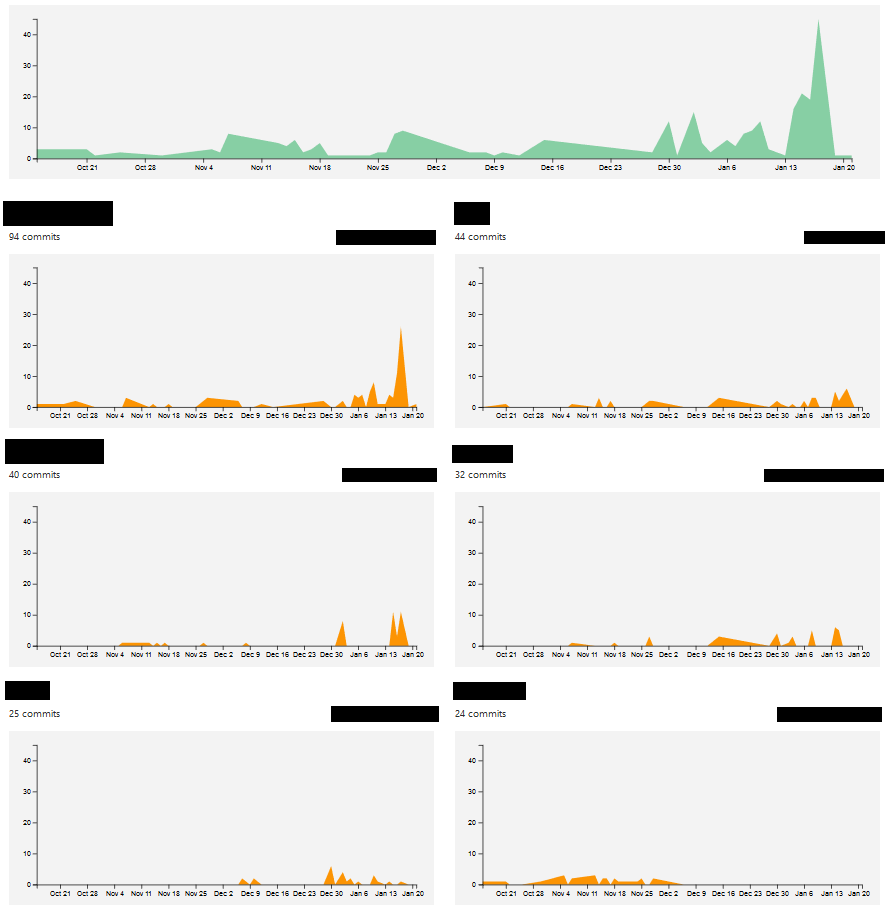
\includegraphics[scale=0.4]{slike/aktivnost.PNG}
			\centering
			\caption{Primjer slike s potpisom}
			\label{fig:promjene}
		\end{figure}
		
		\begin{figure}[H]
			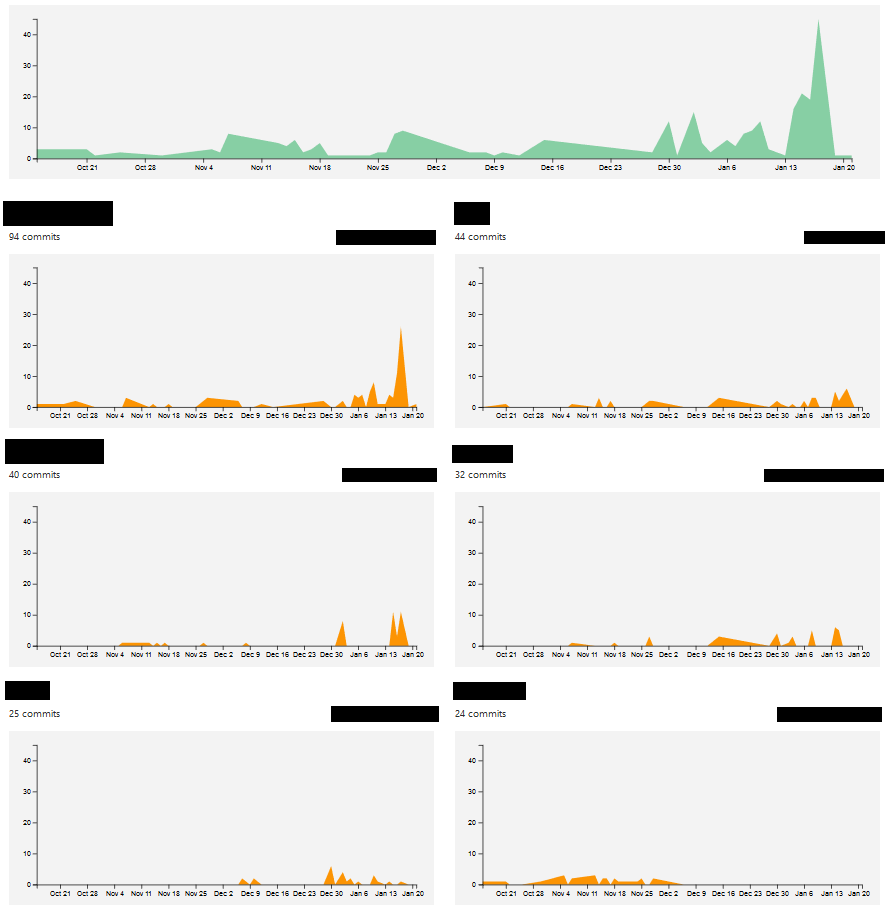
\includegraphics[width=\linewidth]{slike/aktivnost.PNG}
			\caption{Primjer slike s potpisom 2}
			\label{fig:promjene2}
		\end{figure}
		
		
		
		\eject
		
	
	\chapter{Specifikacija programske potpore}
		
	\section{Funkcionalni zahtjevi}
			
			\textbf{\textit{dio 1. revizije}}\\
			
			\textit{Navesti \textbf{dionike} koji imaju \textbf{interes u ovom sustavu} ili  \textbf{su nositelji odgovornosti}. To su prije svega korisnici, ali i administratori sustava, naručitelji, razvojni tim.}\\
				
			\textit{Navesti \textbf{aktore} koji izravno \textbf{koriste} ili \textbf{komuniciraju sa sustavom}. Oni mogu imati inicijatorsku ulogu, tj. započinju određene procese u sustavu ili samo sudioničku ulogu, tj. obavljaju određeni posao. Za svakog aktora navesti funkcionalne zahtjeve koji se na njega odnose.}\\
			
			
			\noindent \textbf{Dionici:}
			
			\begin{packed_enum}
				
				\item Dionik 1
				\item Dionik 2				
				\item ...
				
			\end{packed_enum}
			
			\noindent \textbf{Aktori i njihovi funkcionalni zahtjevi:}
			
			
			\begin{packed_enum}
				\item  \underbar{Aktor 1 (inicijator) može:}
				
				\begin{packed_enum}
					
					\item funkcionalnost 1
					\item funkcionalnost 2
					\begin{packed_enum}
						
						\item  podfunkcionalnost 1 
						\item  podfunkcionalnost 2
				
					\end{packed_enum}
					\item  funkcionalnost 3
					
				\end{packed_enum}
			
				\item  \underbar{Aktor 2 (sudionik) može:}
				
				\begin{packed_enum}
					
					\item funkcionalnost 1
					\item funkcionalnost 2
					
				\end{packed_enum}
			\end{packed_enum}
			
			\eject 
			
			
				
			\subsection{Obrasci uporabe}
				
				\textbf{\textit{dio 1. revizije}}
				
				\subsubsection{Opis obrazaca uporabe}
					\textit{Funkcionalne zahtjeve razraditi u obliku obrazaca uporabe. Svaki obrazac je potrebno razraditi prema donjem predlošku. Ukoliko u nekom koraku može doći do odstupanja, potrebno je to odstupanje opisati i po mogućnosti ponuditi rješenje kojim bi se tijek obrasca vratio na osnovni tijek.}\\
					

					\noindent \underbar{\textbf{UC$<$broj obrasca$>$ -$<$ime obrasca$>$}}
					\begin{packed_item}
	
						\item \textbf{Glavni sudionik: }$<$sudionik$>$
						\item  \textbf{Cilj:} $<$cilj$>$
						\item  \textbf{Sudionici:} $<$sudionici$>$
						\item  \textbf{Preduvjet:} $<$preduvjet$>$
						\item  \textbf{Opis osnovnog tijeka:}
						
						\item[] \begin{packed_enum}
	
							\item $<$opis korak jedan$>$
							\item $<$opis korak dva$>$
							\item $<$opis korak tri$>$
							\item $<$opis korak četiri$>$
							\item $<$opis korak pet$>$
						\end{packed_enum}
						
						\item  \textbf{Opis mogućih odstupanja:}
						
						\item[] \begin{packed_item}
	
							\item[2.a] $<$opis mogućeg scenarija odstupanja u koraku 2$>$
							\item[] \begin{packed_enum}
								
								\item $<$opis rješenja mogućeg scenarija korak 1$>$
								\item $<$opis rješenja mogućeg scenarija korak 2$>$
								
							\end{packed_enum}
							\item[2.b] $<$opis mogućeg scenarija odstupanja u koraku 2$>$
							\item[3.a] $<$opis mogućeg scenarija odstupanja  u koraku 3$>$
							
						\end{packed_item}
					\end{packed_item}

				\noindent \underbar{\textbf{UC2 - Pregled profila benda}}
				\begin{packed_item}
	
						\item \textbf{Glavni sudionik: }Javnost
						\item  \textbf{Cilj:} Pregledati profil benda
						\item  \textbf{Sudionici:} baza podataka,bend
						\item  \textbf{Preduvjet:} /
						\item  \textbf{Opis osnovnog tijeka:}
						
						\item[] \begin{packed_enum}
							\item Javnos odabire profil benda koji želi pregledati
							\item Aplikacija prikazuje profil be
							\item Aplikacija korisniku prikaže recenziju eventa
						\end{packed_enum}
				
				\end{packed_item}
				
				
				\noindent \underbar{\textbf{UC3 - Pregled recenzija}}
				\begin{packed_item}
	
						\item \textbf{Glavni sudionik: }Javnost
						\item  \textbf{Cilj:} Omogućiti pregled recenzija javnosti
						\item  \textbf{Sudionici:} baza podataka
						\item  \textbf{Preduvjet:} /
						\item  \textbf{Opis osnovnog tijeka:}
						
						\item[] \begin{packed_enum}
	
							\item Javna osoba pristupi popisu recenzija evenata
							\item Osoba odabere recenziju koju želi vidjeti
							\item Aplikacija korisniku prikaže recenziju eventa
						\end{packed_enum}
				\end{packed_item}

				
				\noindent \underbar{\textbf{UC4 - Registracija}}
				\begin{packed_item}
	
						\item \textbf{Glavni sudionik: }Korisnik
						\item  \textbf{Cilj:} Registrirati se
						\item  \textbf{Sudionici:} Baza podataka
						\item  \textbf{Preduvjet:} /
						\item  \textbf{Opis osnovnog tijeka:}
						
						\item[] \begin{packed_enum}
	
							\item Korisnik odabire opciju za registraciju
							\item Korisnik unosi potrebne korisničke podatke
							\item Korisnik prima obavijest o uspješnoj registraciji
						\end{packed_enum}
						
						\item[] \begin{packed_item}
	
							\item[1] Odabir već zauzetog korisničkog imena i/ili e-maila, unos podataka u        nedozvoljenom format ili pružanje neispravnog e-maila.
							\item[] \begin{packed_enum}
								
								\item  Sustav obavještava korisnika o neuspjelom upisu i vraća ga na stranicu za registraciju.
								\item Korisnik mijenja potrebne podatke ili odustaje od registracije.

							\end{packed_enum}
						\end{packed_item}						
				\end{packed_item}

				\newpage
				\noindent \underbar{\textbf{UC5 - Prijava u sustav}}
				\begin{packed_item}
	
						\item \textbf{Glavni sudionik: } Administrator, korisnik
						\item  \textbf{Cilj:} Korištenje sustava
						\item  \textbf{Sudionici:} baza podataka
						\item  \textbf{Preduvjet:} Autorizacija korisničkog imena i lozinke
						\item  \textbf{Opis osnovnog tijeka:}
						
						\item[] \begin{packed_enum}
	
							\item Korisnik unosi korisničko ime i lozinku
							\item Baza autorizira unesene podatke
							\item[] \begin{packed_enum}
								
								\item Dozvoljava korisniku korištenje sustava ako su podaci ispravni
								\item   Ne dozvoljava korisniku korištenje sustava ako su podaci ne ispravni
								
							\end{packed_enum}
						\end{packed_enum}
				\end{packed_item}


				\noindent \underbar{\textbf{UC6 - Uvid u popis dodanih instrumenata}}
				\begin{packed_item}
	
						\item \textbf{Glavni sudionik: }Administrator
						\item  \textbf{Cilj:} Pregled dodanih instrumenata od strane glazbenika.Uklanjanje nepotrebnih zapisa u bazi podataka (npr. "Gitara", "gitara")
						\item  \textbf{Sudionici:} baza podataka
						\item  \textbf{Preduvjet:} Glazbenici su dodali svoje instrumente i ti instrumenti su zapisani u bazi podataka
						\item  \textbf{Opis osnovnog tijeka:}
						
						\item[] \begin{packed_enum}
	
							\item Administrator odabire pregled dodanih instrumenata
							\item Ispis dodanih instrumenata
						\end{packed_enum}
				\end{packed_item}


				\noindent \underbar{\textbf{UC9 - Slanje poruka}}
				\begin{packed_item}

					\item \textbf{Glavni sudionik: }Administrator, glazbenik, korisnik
					\item  \textbf{Cilj:} Komunnikacija između korisnika
					\item  \textbf{Sudionici:} Baza podataka
					\item  \textbf{Preduvjet:} Korisnik je prijavljen
					\item  \textbf{Opis osnovnog tijeka:}
					
					\item[] \begin{packed_enum}

							\item Korisnik odabire "poruke"
							\item Aplikacija prikazuje pregled osoba s kojima se već vodio razgovor
							\item Korisnik odabire postojeći razgovor i prikazuju mu se prošle poruke
							\item Korisnik odabire "nova poruka" te pronalazi korisnika kojemu želi poslati poruku
							\item Korisnik odabire polje za pisanje poruke
							\item Korisnik napiše željenu poruku
							\item Korisnik odabere "Pošalji" za slanje poruke
					\end{packed_enum}
				
					\item  \textbf{Opis mogućih odstupanja:}
				
					\item[] \begin{packed_item}

						\item[2.a] Korisnik ima novih poruka
						\item[] \begin{packed_enum}
							\item Ukoliko postoji nova poruka, ime pošiljatelja je podebljano
						\end{packed_enum}
					\end{packed_item}
				\end{packed_item}
			
			\noindent \underbar{\textbf{UC10 - Pisanje recenzija o bendovima}}
			\begin{packed_item}
				
				\item \textbf{Glavni sudionik: }Korisnik
				\item  \textbf{Cilj:} Omogućiti korisnicima aplikacije pisanje recenzija o bendovima
				\item  \textbf{Sudionici:} Baza podataka, bend
				\item  \textbf{Preduvjet:} Korisnik mora biti prijavljen
				\item  \textbf{Opis osnovnog tijeka:} 
				
				\item[] \begin{packed_enum}
					
					\item Korisnik pristupa profilu benda
					\item U okvir za poruku napiše svoje mišljenje o bendu te označi broj zvjezdica kao ocjenu
					\item Korisnik odabere "Završi recenziju"
				\end{packed_enum}
			\end{packed_item}
				
			\noindent \underbar{\textbf{UC11 - Pisanje recenzija za događaje}}
			\begin{packed_item}
				
				\item \textbf{Glavni sudionik: }Korisnik
				\item  \textbf{Cilj:} Napisati recenziju za događaj
				\item  \textbf{Sudionici:} Baza podataka
				\item  \textbf{Preduvjet:} Korisnik je prijavljen
				\item  \textbf{Opis osnovnog tijeka:} 
				
				\item[] \begin{packed_enum}
					
					\item Korisnik odabire opciju za recenziranje događaja
					\item Otvara se prozor za unos recenzije
					\item Korisnik unosi recenziju i potvrđuje se
					\item Recenzija se bilježi na stranici događaja
				\end{packed_enum}
			\end{packed_item}
		 
		    \noindent \underbar{\textbf{UC12 - Pregled profila glazbenika}}
		    \begin{packed_item}
		    	
		    	\item \textbf{Glavni sudionik: }Korisnik, glazbenik
		    	\item  \textbf{Cilj:} Pregled profilne stranice glazbenika 
		    	\item  \textbf{Sudionici:} Baza podataka
		    	\item  \textbf{Preduvjet:} Autorizacija korisničkog imena i lozinke
		    	\item  \textbf{Opis osnovnog tijeka:} 
		    	
		    	\item[] \begin{packed_enum}
		    		
		    		\item Korisnik odabire prikaz profila glazbenika
		    		\item Prikazuju mu se javni podaci glazbenika (kalendar, instrumenti, popis nastupa na kojima svira)
		    	\end{packed_enum}
		    \end{packed_item}
		 
		
		
				
				\subsubsection{Dijagrami obrazaca uporabe}
				
				
				
					
					\textit{Prikazati odnos aktora i obrazaca uporabe odgovarajućim UML dijagramom. Nije nužno nacrtati sve na jednom dijagramu. Modelirati po razinama apstrakcije i skupovima srodnih funkcionalnosti.}
				\eject				
				
				
			\subsection{Sekvencijski dijagrami}
				
				\textbf{\textit{dio 1. revizije}}\\
				
				\textit{Nacrtati sekvencijske dijagrame koji modeliraju najvažnije dijelove sustava (max. 4 dijagrama). Ukoliko postoji nedoumica oko odabira, razjasniti s asistentom. Uz svaki dijagram napisati detaljni opis dijagrama.}
				\eject
	
		\section{Ostali zahtjevi}
		
			\textbf{\textit{dio 1. revizije}}\\
		 
			 \textit{Nefunkcionalni zahtjevi i zahtjevi domene primjene dopunjuju funkcionalne zahtjeve. Oni opisuju \textbf{kako se sustav treba ponašati} i koja \textbf{ograničenja} treba poštivati (performanse, korisničko iskustvo, pouzdanost, standardi kvalitete, sigurnost...). Primjeri takvih zahtjeva u Vašem projektu mogu biti: podržani jezici korisničkog sučelja, vrijeme odziva, najveći mogući podržani broj korisnika, podržane web/mobilne platforme, razina zaštite (protokoli komunikacije, kriptiranje...)... Svaki takav zahtjev potrebno je navesti u jednoj ili dvije rečenice.}
			 
			 
			 
	
	\chapter{Arhitektura i dizajn sustava}
		
	Da bi dugoročno uštedjeli vrijeme, uložili smo dio vremena na konfiguriranje CI (engl. continuous integration) i CD (engl. continuous delivery) procesa. Za isporuku aplikacije odabrali smo Heroku.
	
	Heroku je jedna od najpoznatijih platformi za isporučivanje aplikacija koja se ističe svojom jednostavnošću. Za razliku od AWS-ovih servisa, koje smo također razmatrali, Heroku se sam brine oko instanci i arhitekture sustava na kojem se izvodi naša aplikacija. Zbog ograničenih resursa odlučili smo isporučiti aplikaciju na besplatnu instancu Heroku-a.
	
	Besplatna instanca Heroku-a ima određena ograničenja, a najupečatljivije od njih je način na koji se pokreće projekt.
	Heroku sam prepoznaje kojeg je tipa projekt pa da pokrenemo frontend i backend trebamo dvije instance.
	CD je integriran putem GitLab-ovih pipelinesa za koje je bilo potrebno napisati .gitlab-ci.yml datoteku u kojoj smo konfigurirali GitLab-ov pipeline. GitLab-ov pipeline konfiguriran je tako da se na svaki commit u dev grani izgradi aplikacija, pokrenu i uspješno završe testovi te krene isporuka aplikacije na Heroku.
	
	Da bi osigurali maksimalno vrijeme dostupnosti naše platforme, .yml datoteka također je konfigurirana tako da prilikom commita u master isporuči aplikaciju na druge dvije instance.
	Ukupno imamo četiri pokrenute instance Heroku-a, od koje su dvije backend, a dvije frontend. Backend i frontend imaju svaki svoju razvojnu i produkcijsku instancu. Poveznice na instance:
	\begin{itemize}
		\item \url{http://giger-fer.herokuapp.com/}
		\item \url{https://giger-fer-dev.herokuapp.com/}
		\item \url{https://giger-backend-dev.herokuapp.com/}
		\item \url{http://giger-backend.herokuapp.com/}
	\end{itemize}
	
	
	U skladu s time, Spring Boot aplikacija ima dvije .properties datoteke. Jedna od njih je namijenjena lokalnom izvođenju aplikacije te sadrži postavke lokalne PostgreSQL baze, dok je druga konfigurirana tako da postavke čita iz varijabli okruženja. Varijable okruženja postavljene su na Heroku tako da čak niti pristupom u git repozitorij vanjski korisnik ne može doći do akreditacije (credentials) kojima bi mogao pristupiti bazi.
	
	Prednost ostvarena automatiziranjem procesa isporuke jest povećanje vjerojatnosti uspješnosti iste te povećanje udjela dostupnosti aplikacije zbog dva para instanci servera.
	
	Uvidjevši prednosti korištenja CD-a, primijenili smo to znanje i na prevođenje dokumentacije. 
	Unutar repozitorija, osim pipeline-a za isporuku aplikacije, postoji pipeline za automatsko prevođenje dokumentacije čiji je rezultat .pdf dokument.\\
	Potencijalni prostor za napredak bio bi korištenje Docker tehnologije tako da prilikom pokretanja aplikacije korisnik ne mora imati instaliranu PostgreSQL bazu već ju pokrene u Docker kontejneru.
	
	Od mogućih arhitektura sustava, za svoj projekt smo odabrali objektno usmjerenu arhitekturu. Tu arhitekturu smo odabrali zato što se koristi u industriji te je de facto standard razvoja složenih programskih rješenja. Osim toga, ona je fleksibilna, omogućuje recikliranje koda te logički razdjeljuje sustav na više cjelina, što je bitno s obzirom da više ljudi radi na implementaciji aplikacije. Zahvaljujući modularnosti programskog rješenja, greške su lako ispravljive, a nove mogućnosti dodaju se bez poteškoća.

	Odlučili smo se za web aplikaciju, koja je prilagođena mobilnim uređajima, obzirom da glazbenici, a time i bendovi nemaju uvijek pristup računalu, a ne želimo da je korisnik ograničen samo na mobilne uređaje.\\

	Arhitekturu sustava možemo podijeliti na četiri podsustava:
		\begin{itemize}
			\item Web preglednik
			\item Web poslužitelj
    			\item Web aplikacija
			\item Baza podataka
		\end{itemize}

	
	
	Korisnik (javnost, glazbenik, bend, administrator) pristupa web aplikaciji uz pomoć svog web preglednika, s time da se u sredini nalazi web poslužitelj. Na njemu se nalazi aplikacija koju on pokreće, te uz pomoć protokola komunicira s korisnicima.

	Klijentski (frontend) dio aplikacije omogućuje da korisnik korištenjem sučelja može pristupiti serveru (backend) aplikacije. Ovisno o tome što korisnik hoće, taj server ima mogućnost spajanja na bazu podataka kako bi korisniku prikazao informacije.

	Backend je napisan u Javi 11, a kao razvojni okvir koristimo Java Spring Boot 2.2.0. Dodani su projekti Spring Data JPA kako bi backend mogao lako komunicirati s bazom, Spring Web MVC za rukovanje zahtjevima te Spring Security kako bi zaštitili aplikaciju od vanjskih napada. Za pregledniji kod koristimo Lombok.

	\begin{figure}[H]
		\begin{center}
			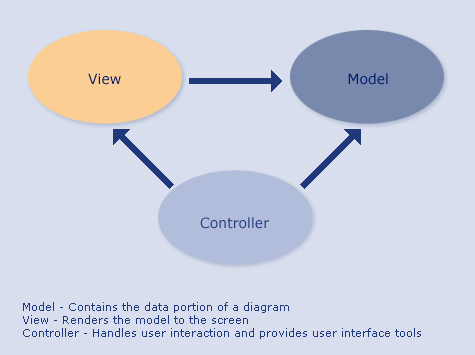
\includegraphics[width=10cm]{slike/mvc.PNG}
		\end{center}
		\caption{Pojednostavljeni prikaz MVC-a}
		\label{fig:mvc}
	\end{figure}

	Za frontend koristimo React. On je moderan i jednostavan framework koji koristi HTML, CSS, JSX i JavaScript uz pomoć kojeg smo napravili sučelje za našu aplikaciju. Uz pomoć React-a možemo lagano komunicirati s backendom koristeći REST.\\




		\section{Baza podataka}
		Za potrebe razvoja \textit{Gigera} koristit će se objektno relacijsko mapiranje. To je metoda koja se koristi u objektno-orijentiranim jezicima te se na taj način stvara virtualna objektna baza podataka. Za implementaciju baze podataka odabrali smo PostgreSQL, zbog generalno pozitivnog iskustva u korištenju te implementacije baze podataka u dosadašnjem fakultetskom obrazovanju. Bitno je naglasiti da na osobnim računalima u svrhu razvijanja aplikacije koristimo istu implementaciju baze kao i na web poslužitelju kako bi minimizirali neočekivano ponašanje.
		
		Baza podataka sastoji se od sljedećih tablica:
		
		\begin{packed_item}
		\item Comment
		\item Message
		\item Conversation
		\item Conversation\_user
		\item System\_person
		\item Person
		\item System\_person\_roles
		\item Organizer
		\item Band
		\item Gig\_type
		\item Band\_occasions
		\item Occasion
		\item Musician\_occasions
		\item Band\_invited\_back\_up\_members
		\item Band\_invited
		\item Band\_back\_up\_members
		\item Musician\_bands
		\item Post
		\item Musician
		\item Instruments
		\item Instrument
		\item Musician\_gig\_history
		\item Gig
		\item Review\_gig
		\item Review
		
	\end{packed_item}
	
	
	\subsection{Opis tablica}
	
	\textbf{Comment}
	Ovaj entitet sadrži jedan komentar. Sadrži atribute: id komentara, id autora, sadržaj te vrijeme objavljivanja. Ovaj entitet je u \textit{Many-to-One} vezi s entitetima: Post i Person.
	\begin{longtabu} to \textwidth {|X[6, l+3]|X[6, l]|X[20, l]|}
		

		\hline \multicolumn{3}{|c|}{\textbf{Comment}}	 \\[3pt] \hline
		\endfirsthead
		
		\hline 
		\endlastfoot
		
		\textbf{id} & BIGINT	&  	jedinstveni identifikator komentara 	\\ \hline
		content & VARCHAR & sadržaj komentara \\ \hline
		posted\_on & TIMESTAMP & datum i vrijeme objave komentara \\ \hline	
		\textit{author\_id} & BIGINT & jedinstveni identifikator autora komentara \\ \hline
		\textit{fk\_post} & BIGINT & jedinstveni identifikator komentara \\ \hline
		
	\end{longtabu}
	
	\textbf{Message}
	Ovaj entitet sadrži informacije o poruci. Sadrži atribute: id poruke, sadržaj poruke, vrijeme kada je poruka poslana, id pošiljatelja i id razgovora. Ovaj entitet je u \textit{Many-to-One} vezi s entitetima: Conversation, Person, Band. Ako je bend poslao poruku, tada je fk\_sender null, a ako ju je poslao korisnik tada je fk\_sender\_band null.
	\begin{longtabu} to \textwidth {|X[6, l+3]|X[6, l]|X[20, l]|}
		
		\hline \multicolumn{3}{|c|}{\textbf{Message}}	 \\[3pt] \hline
		\endfirsthead
		
		\hline
		\endlastfoot
		
		\textbf{id} & BIGINT	&  	jedinstveni identifikator poruke 	\\ \hline
		content	& VARCHAR & sadržaj poruke	\\ \hline
		sent\_time & TIMESTAMP & vrijeme kada je poruka poslana \\ \hline
		\textit{fk\_sender} & BIGINT & jedinstveni identifikator pošiljatelja \\ \hline
		\textit{fk\_sender\_band} & BIGINT & jedinstveni identifikator benda pošiljatelja \\ \hline
		\textit{fk\_converation} & BIGINT & jedinstveni identifikator razgovora \\ \hline
		
	\end{longtabu}
	
	\textbf{Conversation}
	Ovaj entitet sadrži informacije o razgovoru. Sadrži atribute: id razgovora i ime razgovora. Ovaj entitet je u \textit{One-to-Many} vezi s entitetima: Message i
	\emph{Many-to-One} vezi s entitetima: Band i Person.
	\begin{longtabu} to \textwidth {|X[6, l+3]|X[6, l]|X[20, l]|}
		
		\hline \multicolumn{3}{|c|}{\textbf{Conversation}}	 \\[3pt] \hline
		\endfirsthead
		
		\hline
		\endlastfoot
		
		\textbf{id} & BIGINT	&  	jedinstveni identifikator razgovora 	\\ \hline
		\textit{fk\_band} & BIGINT & jedinstveni identifikator benda \\ \hline
		picture\_url & VARCHAR & url slike razgovora \\ \hline
		title	& VARCHAR &  naziv razgovora	\\ \hline
		
	\end{longtabu}
	
	\textbf{Conversation\_user}
	Ova vezna tablica sadrži informacije o sudjelovanju korisniku u razgovoru. Sadrži atribute: id korisnika i id razgovora.
	\begin{longtabu} to \textwidth {|X[6, l+3]|X[6, l]|X[20, l]|}
		
		\hline \multicolumn{3}{|c|}{\textbf{Conversation\_user}}	 \\[3pt] \hline
		\endfirsthead
		
		\hline
		\endlastfoot
		
		\textbf{fk\_user} & BIGINT	&  	jedinstveni identifikator korisnika	\\ \hline
		\textbf{fk\_conversation}	& BIGINT &  jedinstveni identifikator razgovora	\\ \hline
		
	\end{longtabu}
	
	\textbf {System\_Person}
	Ovaj entitet sadrži podatke korisnika potrebne sustavu za sistemsku logiku.  Sadrži atribute: id korisnika, email, locked i verified zastavice te šifriranu lozinku. Ovaj entitet je u \emph{One-to-Many} vezi s entitetom: Roles i \emph{One-to-One} vezi s entitetima: Person, Musician i Organizer.
	\begin{longtabu} to \textwidth {|X[6, l+3]|X[6, l]|X[20, l]|}
		
		\hline \multicolumn{3}{|c|}{\textbf{System\_person}}	 \\[3pt] \hline
		\endfirsthead
		
		\hline
		\endlastfoot
		
		\textbf{id} & BIGINT	&  	jedinstveni identifikator sustavskih podataka o korisniku	\\ \hline
		email & VARCHAR & email adresa osobe \\ \hline
		locked & BOOLEAN & korisnik ima zabranu korištenja aplikacije ili ne \\ \hline
		password\_hash & VARCHAR & hash lozinke osobe \\ \hline
		verified & BOOLEAN & email adresa potvrđena ili ne \\ \hline
		
	\end{longtabu}
	
		\textbf{Person}
	Ovaj entitet sadrži podatke korisnika potrebne za poslovne svrhe.  Sadrži atribute: telefonski broj, url slike korisnika, korisničko ime kojim se predstavlja javnosti. Ovaj entitet je u \emph{One-to-Many} vezi s entitetima: Conversation, Message i
	\emph{One-to-One} vezi s entitetima: Musician, System\_person i Organizer.
	\begin{longtabu} to \textwidth {|X[6, l+3]|X[6, l]|X[20, l]|}
		
		\hline \multicolumn{3}{|c|}{\textbf{Person}}	 \\[3pt] \hline
		\endfirsthead
		
		\hline
		\endlastfoot
		
		\textbf{id} & BIGINT	&  	jedinstveni identifikator korisnika	\\ \hline
		phone\_number & VARCHAR & telefonski broj korisnika \\ \hline
		picture\_url & VARCHAR & url slike korisnika \\ \hline
		username & VARCHAR & korisničko ime korisnika
		
	\end{longtabu}
	
		\textbf{System\_person\_roles}
	Ovo je vezna tablica koja sadrži n-torke iz kojih možemo iščitati dodijeljene uloge pojedinim korisnicima. Sadrži atribute: system\_person\_id i cijeli broj uloge koji predstavlja enumeraciju.
	\begin{longtabu} to \textwidth {|X[6, l+3]|X[6, l]|X[20, l]|}
		
		\hline \multicolumn{3}{|c|}{\textbf{System\_person\_roles}}	 \\[3pt] \hline
		\endfirsthead
		
		\hline
		\endlastfoot
		
		\textbf{system\_person\_id} & BIGINT	&  	jedinstveni identifikator sustavskih podataka o korisniku	\\ \hline
		\textbf{roles} & INT & uloga korisnika \\ \hline
		
		
	\end{longtabu}
	
	\textbf {Organizer}
	Ovaj entitet sadrži informacije o organizatoru. Sadrži atribute: id organizatora te ime organizatora. Ovaj entitet je u \emph{One-to-One} vezi s entitetima: Musician, System\_person i Organizer te u \emph{One-to-Many} vezi s entitetom Gig.
	\begin{longtabu} to \textwidth {|X[6, l+3]|X[6, l]|X[20, l]|}
		
		\hline \multicolumn{3}{|c|}{\textbf{Organizer}}	 \\[3pt] \hline
		\endfirsthead
		
		\hline
		\endlastfoot
		
		\textbf{id} & BIGINT	&  	jedinstveni identifikator organizatora 	\\ \hline
		manager\_name	& VARCHAR &  ime organizatora	\\ \hline
		
	\end{longtabu}

\textbf{Band}
Ovaj entitet sadrži podatke o kreiranom bendu.  Sadrži atribute: id, opis, datum formiranja, adresu sjedišta, dodatni opis adrese, par koordinata, maksimalnu udaljenost, naziv benda, url slike benda i id voditelja benda. Ovaj entitet je u \textit{Many-to-Many} vezi s Musician za potrebe liste članova, u \textit{Many-to-One} vezi s Musician za potrebu evidencije voditelja benda te \emph{One-to-Many} vezi s entitetima: Message, Conversation, Gig i Post.

	\begin{longtabu} to \textwidth {|X[6, l+3]|X[6, l]|X[20, l]|}
		
		\hline \multicolumn{3}{|c|}{\textbf{Band}}	 \\[3pt] \hline
		\endfirsthead
		
		\hline 
		\endlastfoot
		
		\textbf{id} & BIGINT	&  	jedinstveni identifikator benda 	\\ \hline
		bio & VARCHAR & opis benda \\ \hline
		formed\_date & DATE & datum osnutka benda \\ \hline
		address & VARCHAR & adresa benda \\ \hline
		extra\_description & VARCHAR & dodatak opis benda \\ \hline
		x & DOUBLE & x koordinata lokacije \\ \hline
		y & DOUBLE & y koordinata lokacije \\ \hline
		max\_distance & DOUBLE & najveća udaljenost koju bend želi prijeći zbog gaže \\ \hline
		name & VARCHAR & ime benda \\ \hline
		picture\_url & VARCHAR & url slike benda \\ \hline
		\textit{leader\_id}	& BIGINT &  jedinstveni identifikator voditelja benda	\\ \hline 	
		
	\end{longtabu}
	
			\textbf {Gig\_type}
	Ovo je vezna tablica iz koje se mogu iščitati sve vrste nastupa koje izvodi određeni bend. Sadrži atribute: band\_id i naziv tipa nastupa.
	\begin{longtabu} to \textwidth {|X[6, l+3]|X[6, l]|X[20, l]|}

		\hline \multicolumn{3}{|c|}{\textbf{Gig\_type}}	 \\[3pt] \hline
		\endfirsthead

		\hline
		\endlastfoot

		\textbf{band\_id} &  BIGINT	&  	jedinstveni identifikator benda 	\\ \hline
		\textbf{gig\_type}	& VARCHAR &  vrsta nastupa	\\ \hline

	\end{longtabu}

				\textbf {Band\_occasions}
	Ovo je vezna tablica iz koje se može iščitati zauzetost benda. Sadrži atribute: identifikator benda i identifikator termina.
	\begin{longtabu} to \textwidth {|X[6, l+3]|X[6, l]|X[20, l]|}

		\hline \multicolumn{3}{|c|}{\textbf{Band\_occasions}}	 \\[3pt] \hline
		\endfirsthead

		\hline
		\endlastfoot

		\textbf{occasion\_id} &  BIGINT	&  	jedinstveni identifikator događaja 	\\ \hline
		\textbf{band\_id} &  BIGINT	&  	jedinstveni identifikator benda koji sudjeluje na događaju 	\\ \hline

	\end{longtabu}


		\textbf{Occasion}
	Ovaj entitet sadrži podatke o događaju. Sadrži atribute: id događaja, opis, datum, zastavicu privatnosti. Ovaj entitet je u \textit{Many-to-One} vezi s entitetima: Musician i Band.
	\begin{longtabu} to \textwidth {|X[6, l+3]|X[6, l]|X[20, l]|}
		
		\hline \multicolumn{3}{|c|}{\textbf{Occasion}}	 \\[3pt] \hline
		\endfirsthead
		
		\hline 
		\endlastfoot
		
		\textbf{id} &  BIGINT	&  	jedinstveni identifikator događaja 	\\ \hline
		description & VARCHAR & opis događaja \\ \hline
		local\_date & DATE & datum održavanja događaja \\ \hline
		personal\_occasion & BOOLEAN & privatan događaj ili ne \\ \hline

		
		
	\end{longtabu}
	
		\textbf{Musician\_occasions}
	Ovo je vezna tablica iz koje se može iščitati zauzetost glazbenika. Sadrži atribute: identifikator glazbenika i identifikator termina.
	\begin{longtabu} to \textwidth {|X[6, l+3]|X[6, l]|X[20, l]|}
		
		\hline \multicolumn{3}{|c|}{\textbf{Musician\_occasions}}	 \\[3pt] \hline
		\endfirsthead
		
		\hline 
		\endlastfoot
		
		\textbf{musician\_id} &  BIGINT	&  	jedinstveni identifikator glazbenika 	\\ \hline
		\textbf{occasions\_id} &  BIGINT	&  	jedinstveni identifikator termina	\\ \hline
		
		
	\end{longtabu}
	
		\textbf{Band\_invited\_back\_up\_members}
	Ovo je vezna tablica iz koje se mogu iščitati poslane i neodgovorene pozivnice za pričuvnog člana benda. Sadrži atribute: identifikator glazbenika i identifikator benda.
	\begin{longtabu} to \textwidth {|X[6, l+11]|X[6, l]|X[20, l]|}
		
		\hline \multicolumn{3}{|c|}{\textbf{Band\_invited\_back\_up\_members}}	 \\[3pt] \hline
		\endfirsthead
		
		\hline 
		\endlastfoot
		
		\textbf{band\_id} &  BIGINT	&  	jedinstveni identifikator benda 	\\ \hline
		\textbf{invited\_back\_up\_members\_id} &  BIGINT	&  	jedinstveni identifikator glazbenika pozvanih u bend kao pričuvni član	\\ \hline
		
		
	\end{longtabu}
	
		\textbf{Band\_invited}
	Ovo je vezna tablica iz koje se mogu iščitati poslane i neodgovorene pozivnice za člana benda. Sadrži atribute: identifikator glazbenika i identifikator benda.
	\begin{longtabu} to \textwidth {|X[6, l+3]|X[6, l]|X[20, l]|}
		
		\hline \multicolumn{3}{|c|}{\textbf{Band\_invited}}	 \\[3pt] \hline
		\endfirsthead
		
		\hline 
		\endlastfoot
		
		\textbf{band\_id} &  BIGINT	&  	jedinstveni identifikator benda 	\\ \hline
		\textbf{invited\_id} &  BIGINT	&  	jedinstveni identifikator glazbenika pozvanih u bend	\\ \hline
		
		
	\end{longtabu}
	
			\textbf {Band\_back\_up\_members}
	Ovo je vezna tablica iz koje se mogu iščitati pričuvni članovi bendova. Sadrži atribute: identifikator glazbenika i identifikator benda.
	\begin{longtabu} to \textwidth {|X[6, l+11]|X[6, l]|X[20, l]|}
		
		\hline \multicolumn{3}{|c|}{\textbf{Band\_back\_up\_members}}	 \\[3pt] \hline
		\endfirsthead
		
		\hline 
		\endlastfoot
		
		\textbf{band\_id} &  BIGINT	&  	jedinstveni identifikator benda 	\\ \hline
		\textbf{invited\_back\_up\_members\_id} &  BIGINT	&  	jedinstveni identifikator glazbenika koji su pričuvni članovi	\\ \hline
		
		
	\end{longtabu}
	
			\textbf {Musician\_bands}
	Ovo je vezna tablica iz koje se mogu iščitati članovi bendova. Sadrži atribute: identifikator glazbenika i identifikator benda.
	\begin{longtabu} to \textwidth {|X[6, l+3]|X[6, l]|X[20, l]|}
		
		\hline \multicolumn{3}{|c|}{\textbf{Musician\_bands}}	 \\[3pt] \hline
		\endfirsthead
		
		\hline 
		\endlastfoot
		
		\textbf{fk\_musician} & BIGINT	&  	jedinstveni identifikator glazbenika 	\\ \hline
		\textbf{fk\_band}	& BIGINT &  jedinstveni identifikator benda	\\ \hline
		
	\end{longtabu}
	
	\textbf{Post}
	Ovaj entitet sadrži podatke o objavi. Sadrži atribute: id objave, sadržaj, datum i vrijeme objave, identifikator korisnika ili benda (autora). Ovaj entitet je u \textit{One-to-Many} vezi s entitetima: Comment te u \emph{Many-to-one} s entitetima: Person, Band.
	\begin{longtabu} to \textwidth {|X[6, l+3]|X[6, l]|X[20, l]|}
		
		\hline \multicolumn{3}{|c|}{\textbf{Post}}	 \\[3pt] \hline
		\endfirsthead
		
		\hline 
		\endlastfoot
		
		\textbf{id} & BIGINT	&  	jedinstveni identifikator objave 	\\ \hline
		content & VARCHAR & sadržaj objave \\ \hline
		published\_on & TIMESTAMP & datum i vrijeme objave \\ \hline
		\textit{fk\_band} & BIGINT & jedinstveni identifikator benda \\ \hline
		\textit{fk\_user} & BIGINT & jedinstveni identifikator korisnika koji je napisao objavu \\ \hline
		
	\end{longtabu}
	
		\textbf {Musician}
	Ovaj entitet sadrži informacije o glazbeniku. Sadrži atribute: id glazbenika, oznaku za privatan kalendar te opis glazbenika. Ovaj entitet je u \emph{One-to-One} vezi s entitetima: System\_person, Organizer i Person, u \emph{Many-to-Many} vezi s entitetima: Instrument i Band te u \emph{One-to-Many} vezi s entitetima: Band (u potrebe pohranjivanja voditelja benda) i Occasions.
	\begin{longtabu} to \textwidth {|X[6, l+3]|X[6, l]|X[20, l]|}
		
		\hline \multicolumn{3}{|c|}{\textbf{Musician}}	 \\[3pt] \hline
		\endfirsthead
		
		\hline 
		\endlastfoot
		
		\textbf{id} & BIGINT	&  	jedinstveni identifikator glazbenika 	\\ \hline	
		bio	& VARCHAR &  opis glazbenika	\\ \hline 
		public\_calendar & BOOLEAN & kalendar glazbenika javan ili ne \\ \hline
			
		
	\end{longtabu}
	
	\textbf{Instruments}
	Ovo je vezna tablica iz koje se može iščitati koje instrumente svira pojedini glazbenik. Sadrži atribute: id instrumenta te id glazbenika.
	\begin{longtabu} to \textwidth {|X[6, l+3]|X[6, l]|X[20, l]|}
		
		\hline \multicolumn{3}{|c|}{\textbf{Instruments}}	 \\[3pt] \hline
		\endfirsthead
		
		\hline 
		\endlastfoot
		
		\textbf{instruments\_id} & BIGINT & jedinstveni identifikator instrumenta \\ \hline
		\textbf{musician} & BIGINT	&  	jedinstveni identifikator glazbenika	\\ \hline
		
		
	\end{longtabu}
	
	\textbf{Instrument}
	Ovaj entitet sadrži informacije o instrumentima. Sadrži atribute: id instrumenta, ime instrumenta te vrstu instrumenta. Ovaj entitet je u \emph{One-to-Many} vezi s entitetom Musician.
	\begin{longtabu} to \textwidth {|X[6, l+3]|X[6, l]|X[20, l]|}
		
		\hline \multicolumn{3}{|c|}{\textbf{Instrument}}	 \\[3pt] \hline
		\endfirsthead
		
		\hline 
		\endlastfoot
		
		\textbf{id} & BIGINT & jedinstveni identifikator instrumenta \\ \hline
		name & VARCHAR & ime instrumenta \\ \hline
		type & INT & vrsta instrumenta \\ \hline
		
		
	\end{longtabu}
	
		\textbf{Musician\_gig\_history}
	Ovo je vezna tablica iz koje se može iščitati povijest nastupa glazbenika. Sadrži atribute: identifikator glazbenika i identifikator nastupa.
	\begin{longtabu} to \textwidth {|X[6, l+3]|X[6, l]|X[20, l]|}
		
		\hline \multicolumn{3}{|c|}{\textbf{Musician\_gig\_history}}	 \\[3pt] \hline
		\endfirsthead
		
		\hline 
		\endlastfoot
		
		\textbf{fk\_musician} & BIGINT & jedinstveni identifikator glazbenika \\ \hline
		\textbf{fk\_gig} & BIGINT & jedinstveni identifikator nastupa \\ \hline
		
		
		
	\end{longtabu}
	
	\textbf {Gig}
	Ovaj entitet sadrži informacije o nastupima. Sadrži atribute: id nastupa, datum i vrijeme održavanja nastupa, opis nastupa, očekivano trajanje nastupa, oznaku za postignut dogovor, vrstu nastupa, adresa održavanja nastupa, dodatan opis nastupa, x koordinata lokacije, y koordinata lokacije, oznaku za privatan nastup, preporučenu cijenu ulaznice, id organizatora te id benda. Ovaj entitet je u \textit{Many-to-One} vezi s entitetima Organizer i Band te \textit{One-to-Many} vezi s entitetom Review i u \emph{Many-to-Many} vezi s entitetom Musician.
	\begin{longtabu} to \textwidth {|X[6, l+3]|X[6, l]|X[20, l]|}
		
		\hline \multicolumn{3}{|c|}{\textbf{Gig}}	 \\[3pt] \hline
		\endfirsthead
		
		\hline 
		\endlastfoot
		
		\textbf{id} & BIGINT	&  	jedinstveni identifikator nastupa 	\\ \hline
		date\_time & TIMESTAMP & datum i vrijeme održavanja nastupa \\ \hline
		description & VARCHAR & opis nastupa \\ \hline
		expected\_duration & VARCHAR & očekivano trajanje nastupa \\ \hline
		final\_deal\_achieved & BOOLEAN & dogovor postignut ili ne \\ \hline
		gig\_type & INT & vrsta nastupa \\ \hline
		address & VARCHAR & adresa održavanja nastupa \\ \hline
		extra\_description & VARCHAR & dodatan opis nastupa \\ \hline
		x & DOUBLE & x koordinata lokacije \\ \hline
		y & DOUBLE & y koordinata lokacije \\ \hline
		private\_gig & BOOLEAN & nastupa privatan ili ne \\ \hline
		proposed\_price & INT & preporučena cijena ulaznice \\ \hline
		\textit{organizer\_id}	& BIGINT &  jedinstveni identifikator organizatora	\\ \hline 	
		\textit{band\_id}	& BIGINT &  jedinstveni identifikator benda	\\ \hline 	
		
	\end{longtabu}
	
	\textbf {Review\_gig}
	Ovo je vezna tablica iz koje pronalazimo pripadnost recenzije pojedinom nastupu. Sadrži atribute: id nastupa i id recenzije.
	\begin{longtabu} to \textwidth {|X[6, l+3]|X[6, l]|X[20, l]|}
		
		\hline \multicolumn{3}{|c|}{\textbf{Review\_gig}}	 \\[3pt] \hline
		\endfirsthead
		
		\hline 
		\endlastfoot
		
		\textbf{fk\_gig} & BIGINT	&  	jedinstveni identifikator nastupa 	\\ \hline
		\textbf{fk\_review}	& BIGINT &  jedinstveni identifikator recenzije	\\ \hline 		
		
	\end{longtabu}
	
	\textbf{Review}
	Ovaj entitet sadrži informacije za recenziju. Sadrži atribute: id recenzije, sadržaj recenzije benda, sadržaj recenzije organizatora, vrijeme objave recenzije, ocjenu benda, ocjenu organizatora te id autora. Ovaj entitet je u \emph{Many-to-One} vezi s entitetima: Musician i Organizer.
	
	\begin{longtabu} to \textwidth {|X[6, l+14]|X[6, l+2]|X[20, l]|}
		
		\hline \multicolumn{3}{|c|}{\textbf{Review}}	 \\[3pt] \hline
		\endfirsthead
		
		\hline
		\endlastfoot
		
		\textbf{id} & BIGINT	&  	jedinstveni identifikator recenzije 	\\ \hline
		content\_of\_review\_for\_band	& VARCHAR &  sadržaj komentara benda	\\ \hline
		content\_of\_review\_for\_organizer	& VARCHAR &  sadržaj komentara organizatora	\\ \hline
		created & TIMESTAMP & vrijeme objave komentara \\ \hline
		grade\_band & INT & ocjena benda \\ \hline
		grade\_organizer & INT & ocjena organizatora  \\ \hline
		\textit{author\_id} & BIGINT	& jedinstveni identifikator korisnika koji je autor recenzije	\\ \hline
		
		
	\end{longtabu}
	

		
	

			
			\subsection{Dijagram baze podataka}
			
			\begin{figure}[H]
			\begin{center}
				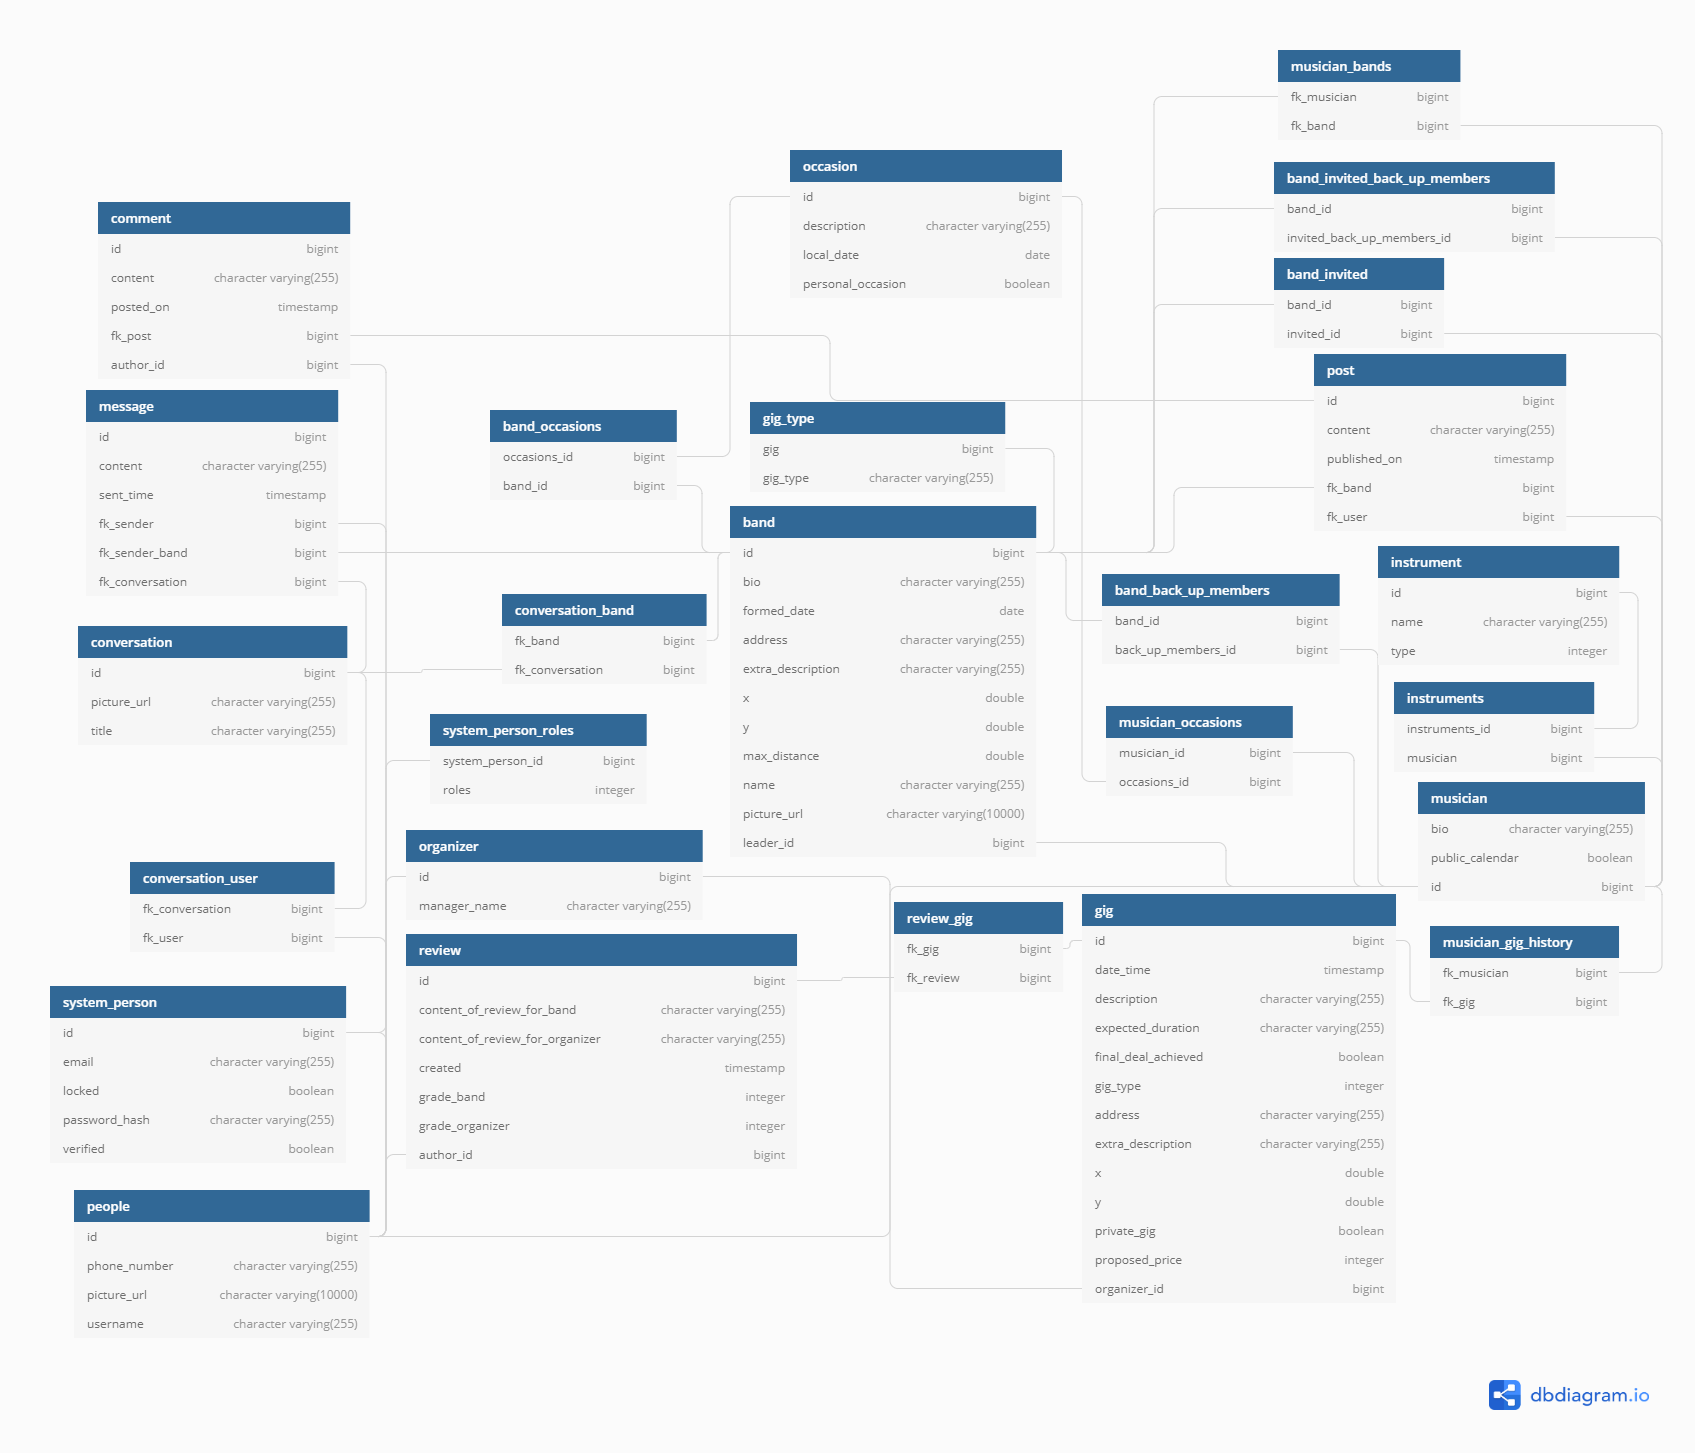
\includegraphics[width=17cm]{slike/ERModel.PNG}
			\end{center}
			\caption{Dijagram baze podataka}
			\label{fig:dijagramBaze}
		\end{figure}
			
			
			
		\section{Dijagram razreda}


			\textit{\textbf{dio 2. revizije}} \\
			
			\textit{Prilikom druge predaje projekta dijagram razreda i opisi moraju odgovarati stvarnom stanju implementacije} \\
			
			
			Na slici 4.3 prikazan je Controllers dio backend aplikacije. Controlleri su jedina izložena točka u aplikaciji te nad njima frontend izvršava upite. Svi Controller-i su zaštićeni Spring Security-jem te se prije svakog propuštanja zahtjeva na Controller autorizira token koji se nalazi u zaglavlju zahtjeva. Jedina iznimka su Controller-i koji služe za registraciju i prijavu. Nakon što se zahtjev autorizira Controller-i pozivaju servisni sloj aplikacije te od njih zahtjevaju da izvrše dio poslovne logike za koju su napisani. Povratni tip Controller-a su DTO-ovi (Data Transfer Objects) prikazani na slici 4.4. Njima se na frontend vraća samo dio informacije prikupljene od servisa.  

			\begin{figure}[H]
				\begin{center}
					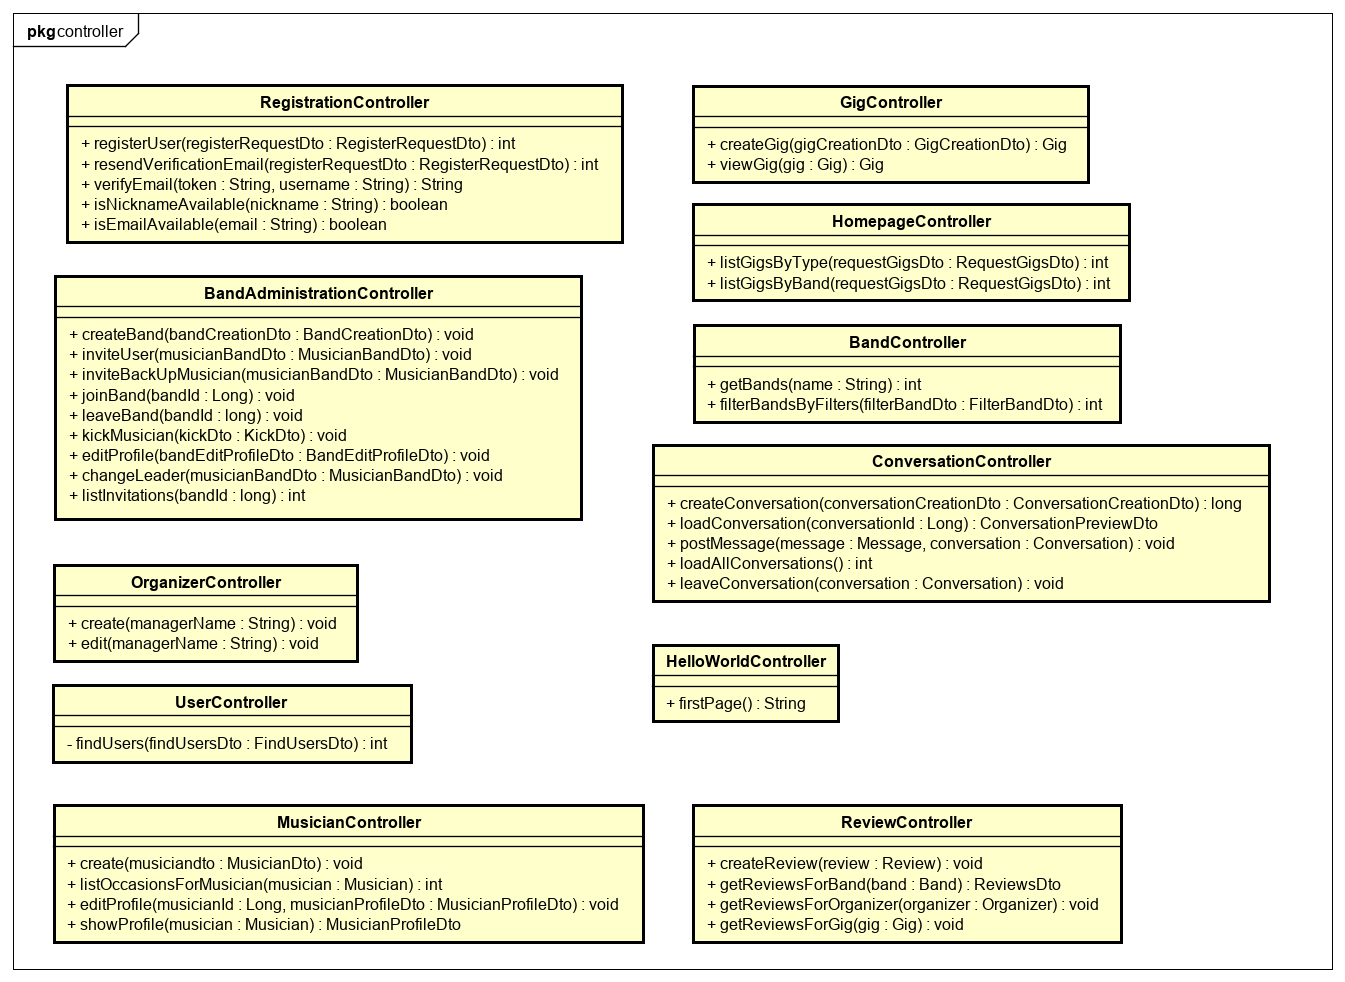
\includegraphics[width=17cm]{slike/kontroleri.PNG}
				\end{center}
				\caption{Dijagram razreda - dio Controllers}
				\label{fig:kontroleri}
			\end{figure}
		
			Slika 4.4 prikazuje DTO-ove kojima backend dio aplikacije komunicira s frontendom. DTO-ove smo modelirali tako da izbjegnemo kružne reference objekata koje dobijemo iz baze podataka. Kao posljedica, DTO-ovi sadrže uglavnom primitivne tipove ili neke druge DTO-ove (npr. ConversationPreviewDTO sadrži listu PersonPreviewDTO koji predstavljaju sudionike razgovora). DTO-ove koristimo u oba smjera komunikacije backenda i frontenda.
			
			
			\begin{figure}[H]
				\begin{center}
					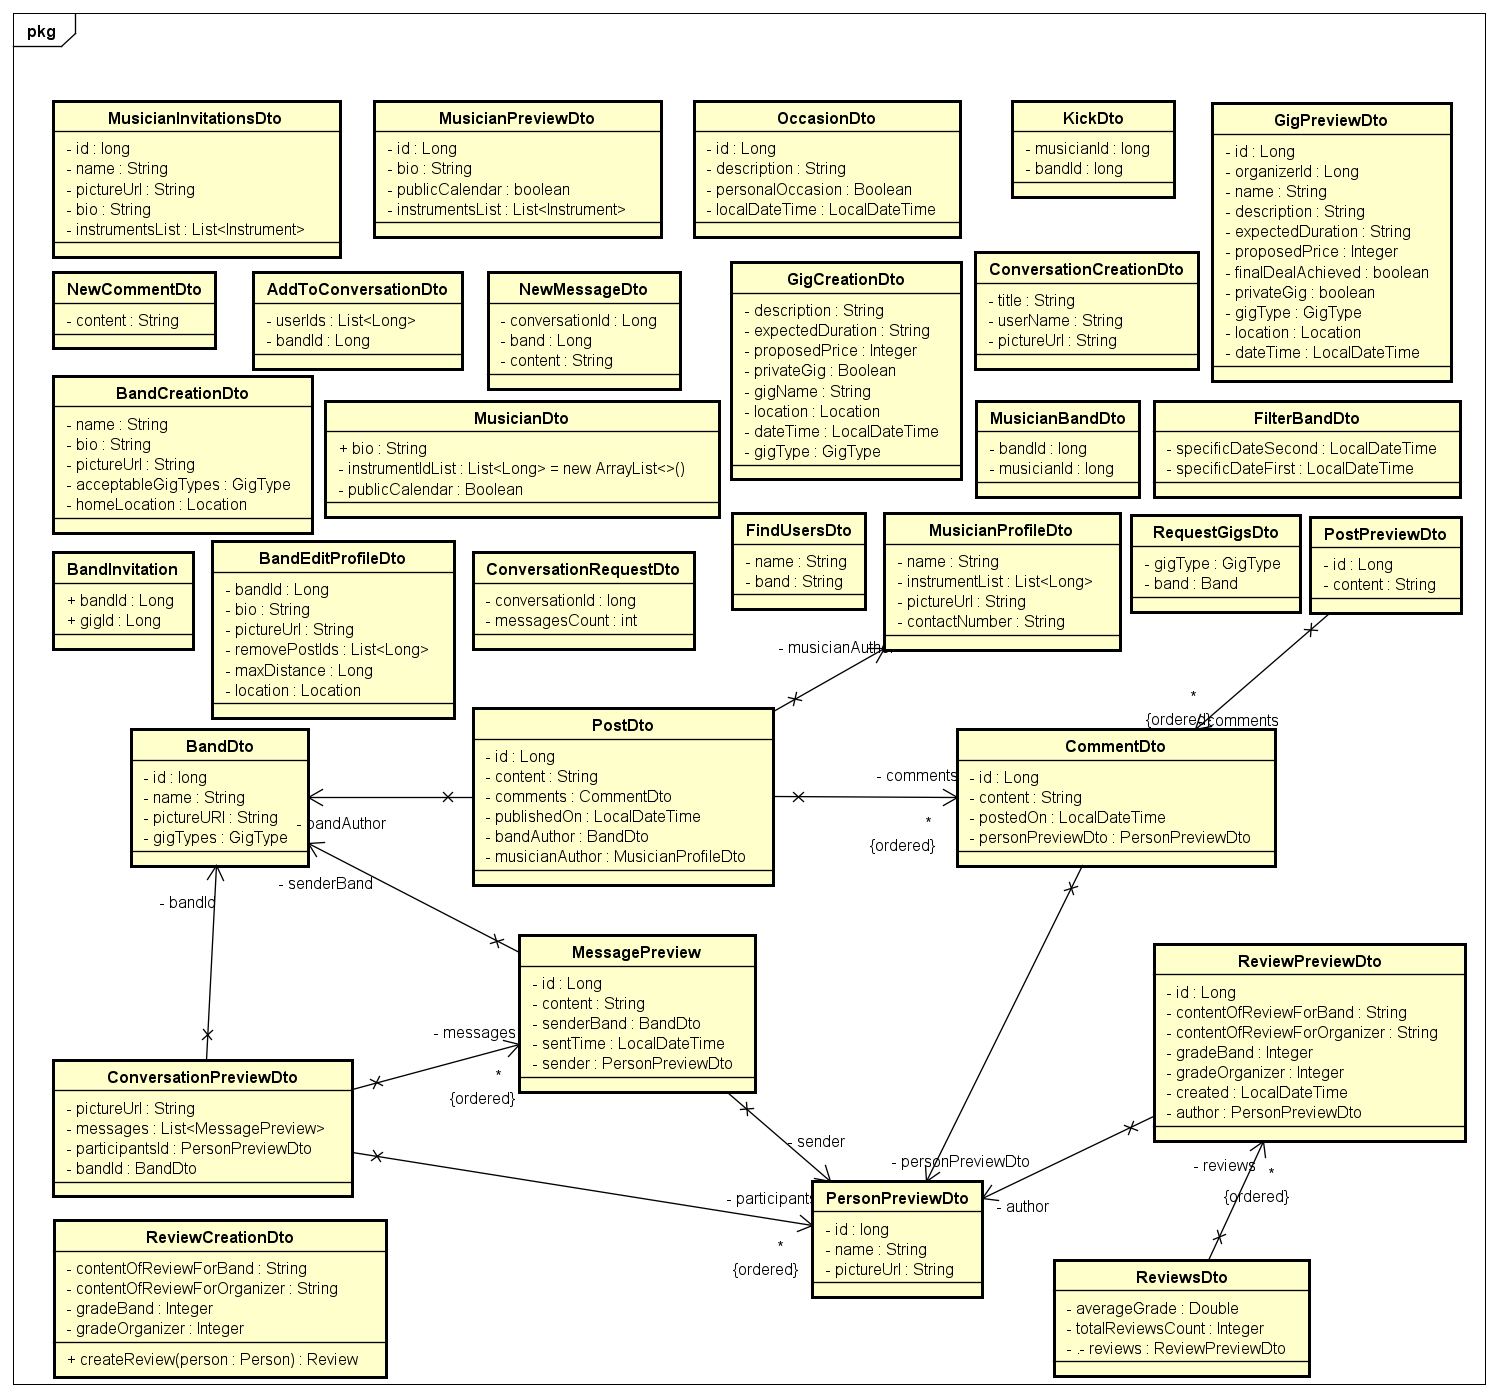
\includegraphics[width=17cm]{slike/pravi_dto2.PNG}
				\end{center}
				\caption{Dijagram razreda - dio Data transfer objects}
				\label{fig:dto}
			\end{figure}
		
		Slika 4.5 prikazuje dijagram razreda servisnog sloja. Servisi komuniciraju s repozitorijima koji pristupaju bazi i Controller-ima od kojih dobivaju i kojima vraćaju podatke. Servisi iz baze dobivaju instance objekata koji mogu biti povezani s drugim podatcima, itd. i njihov je cilj poštivajući poslovnu logiku obraditi te podatke i kao rezultat svog izvođenja vraćaju DTO-ove. Servisi sadrže svu poslovnu logiku. Gotovo svaki Controller ima pripadajući servis, a svaki je servis logički objedinjen skup funkcija poslovne logike. Iznimke koje se bacaju u servisima omataju se GigerException-om koji nasljeđuje RuntimeException. Ako se pogreška propagira iz sustava, možemo provjeriti njezin tip te ako je zamotana u GigerException, znači da je to iznimka koju smo očekivali, u protivnom je došlo do neočekivane situacije u sustavu.
		
		\begin{figure}[H]
			\begin{center}
				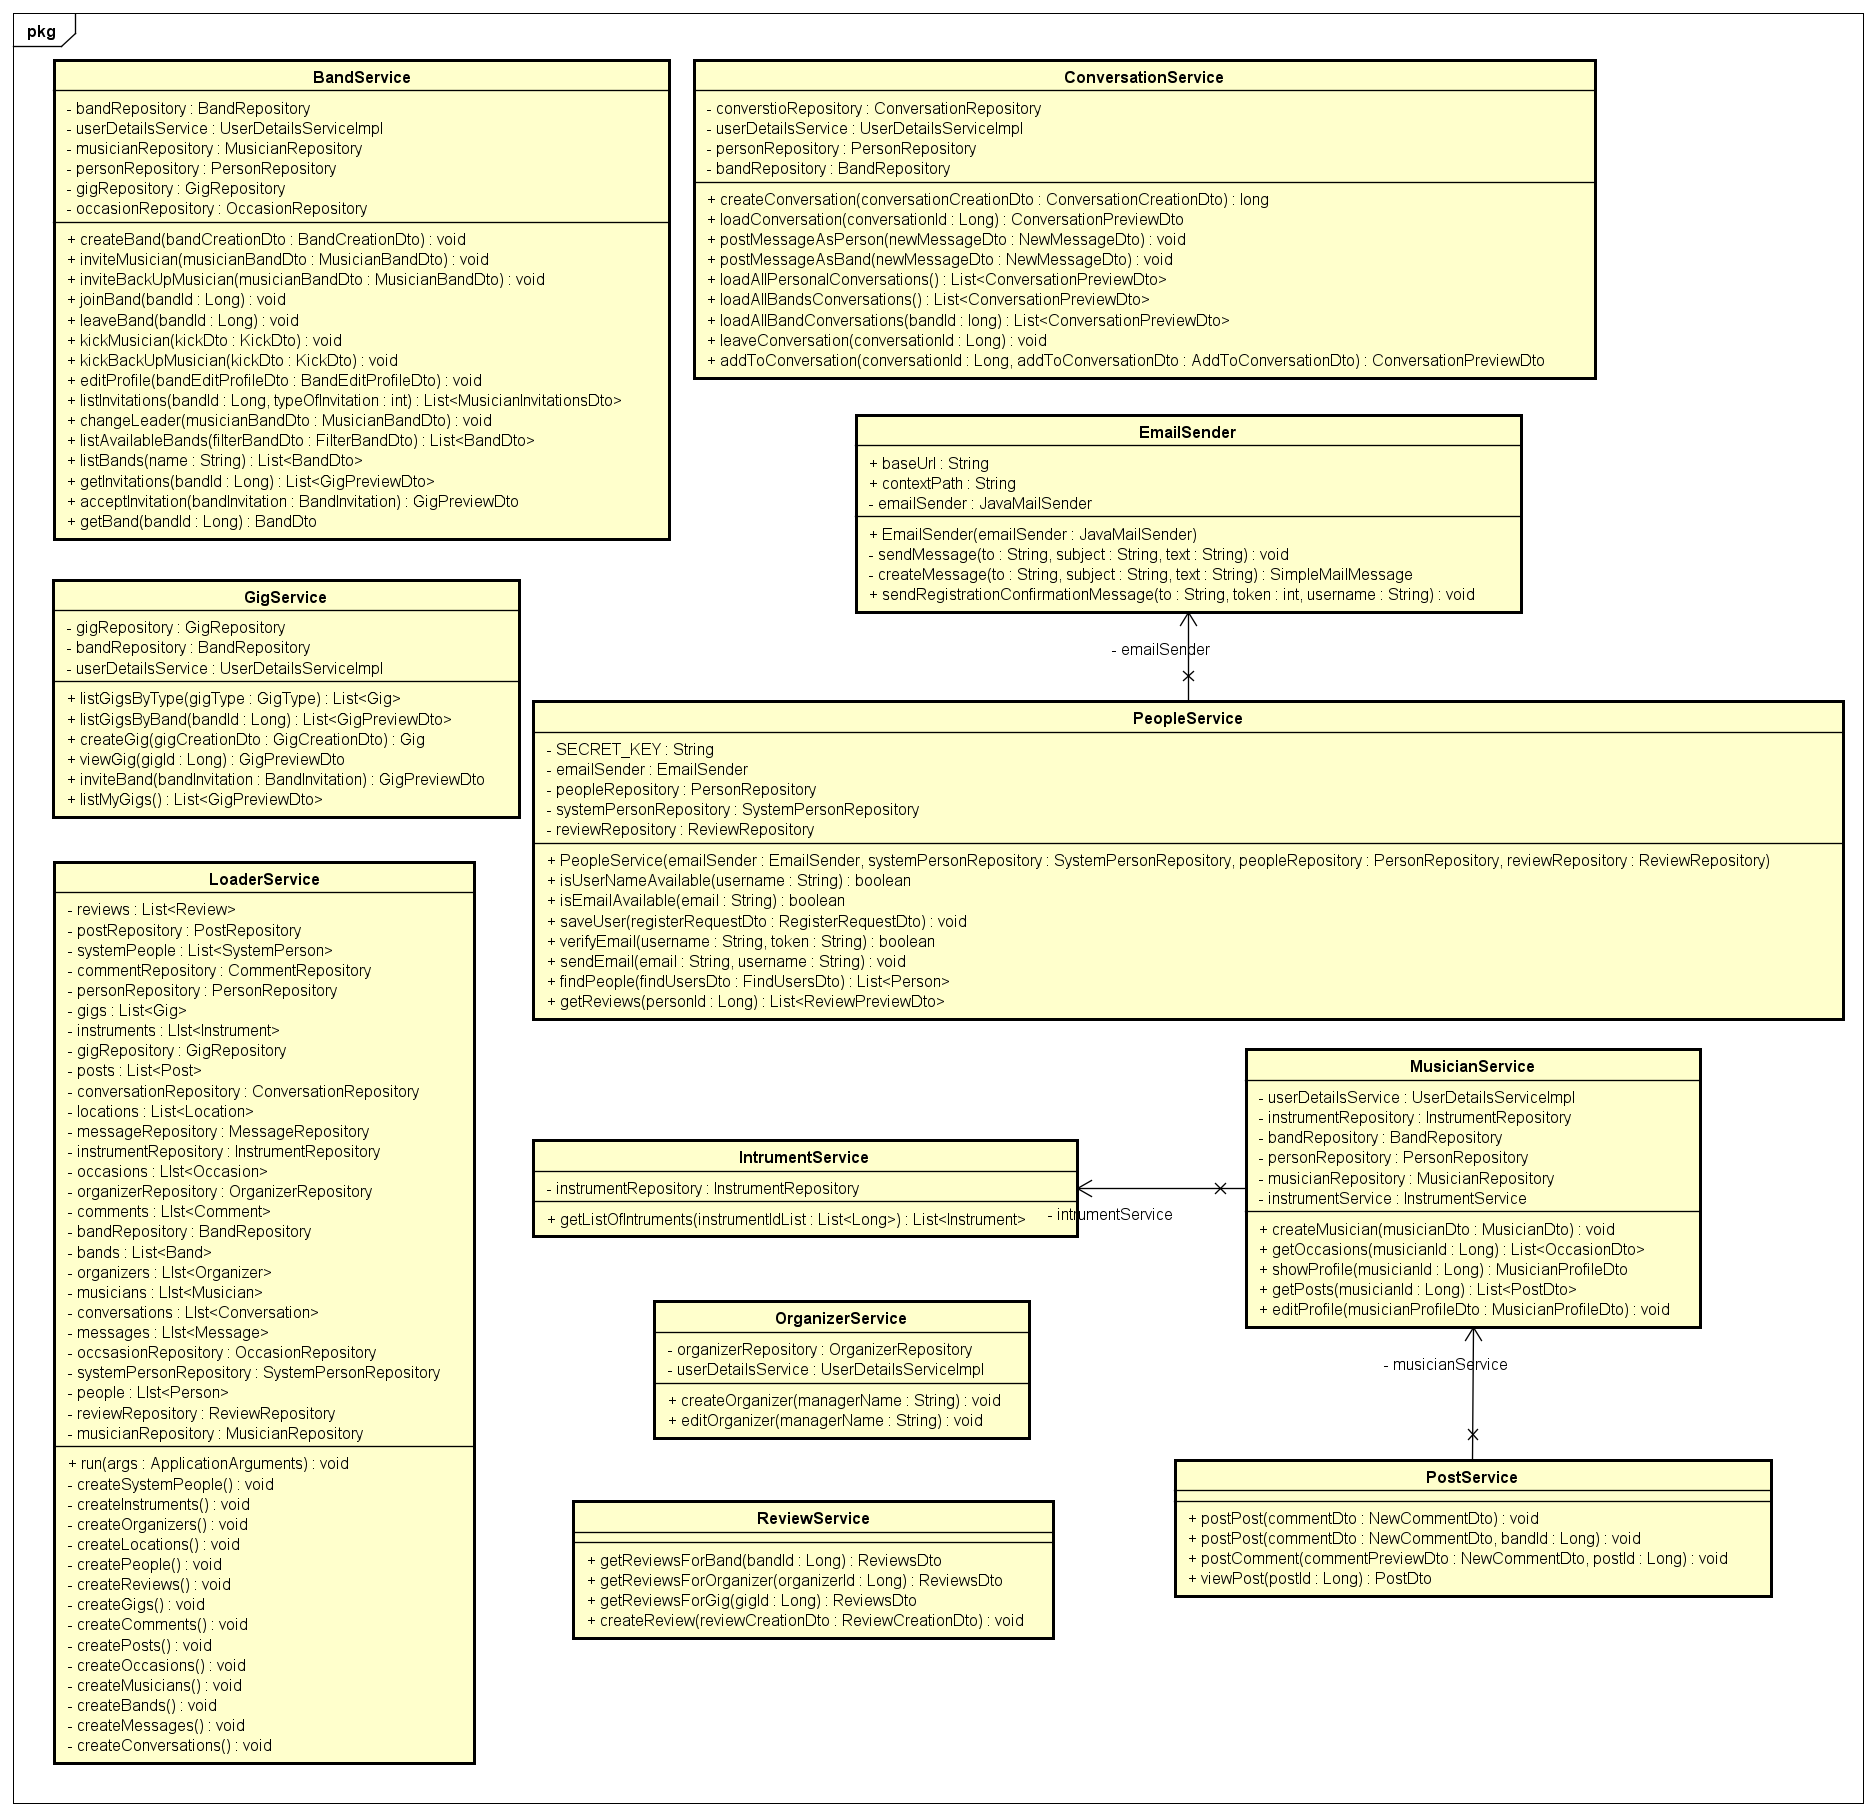
\includegraphics[width=16cm]{slike/service.PNG}
			\end{center}
			\caption{Dijagram razreda - dio Service}
			\label{fig:service}
		\end{figure}
	
	
	Slika 4.6 prikazuje razrede koji predstavljaju enitete enitetsko -  relacijskog modela u bazi podataka. Razred Band predstavlja bend kojim upravlja glazbenik koji je postavljen za voditelja benda. Razred SystemPerson predstavlja razred u kojem su objedinjeni svi sustavski podaci vezani za osobu kao što su: email, hash lozinke i id. Gig predstavlja  nastup nekog benda koji organizira određeni organizator i pri tom enkapsulira sve logističke informacije o tom nastupu. Razred Conversation omogućuje komunikaciju između aktora glazbenika i organizatora.
	Glazbenik je opisan razredom Musician, dok je organizator opisan razredom Organizer. Razredi Post, Comment, Location, Instrument, Message služe za enkapsulaciju informacija kako bi dopunili razrede poput Band, Conversation i Musician. GigType i Role predstavljaju enumeracije.
	
	
		\begin{figure}[H]
			\begin{center}
				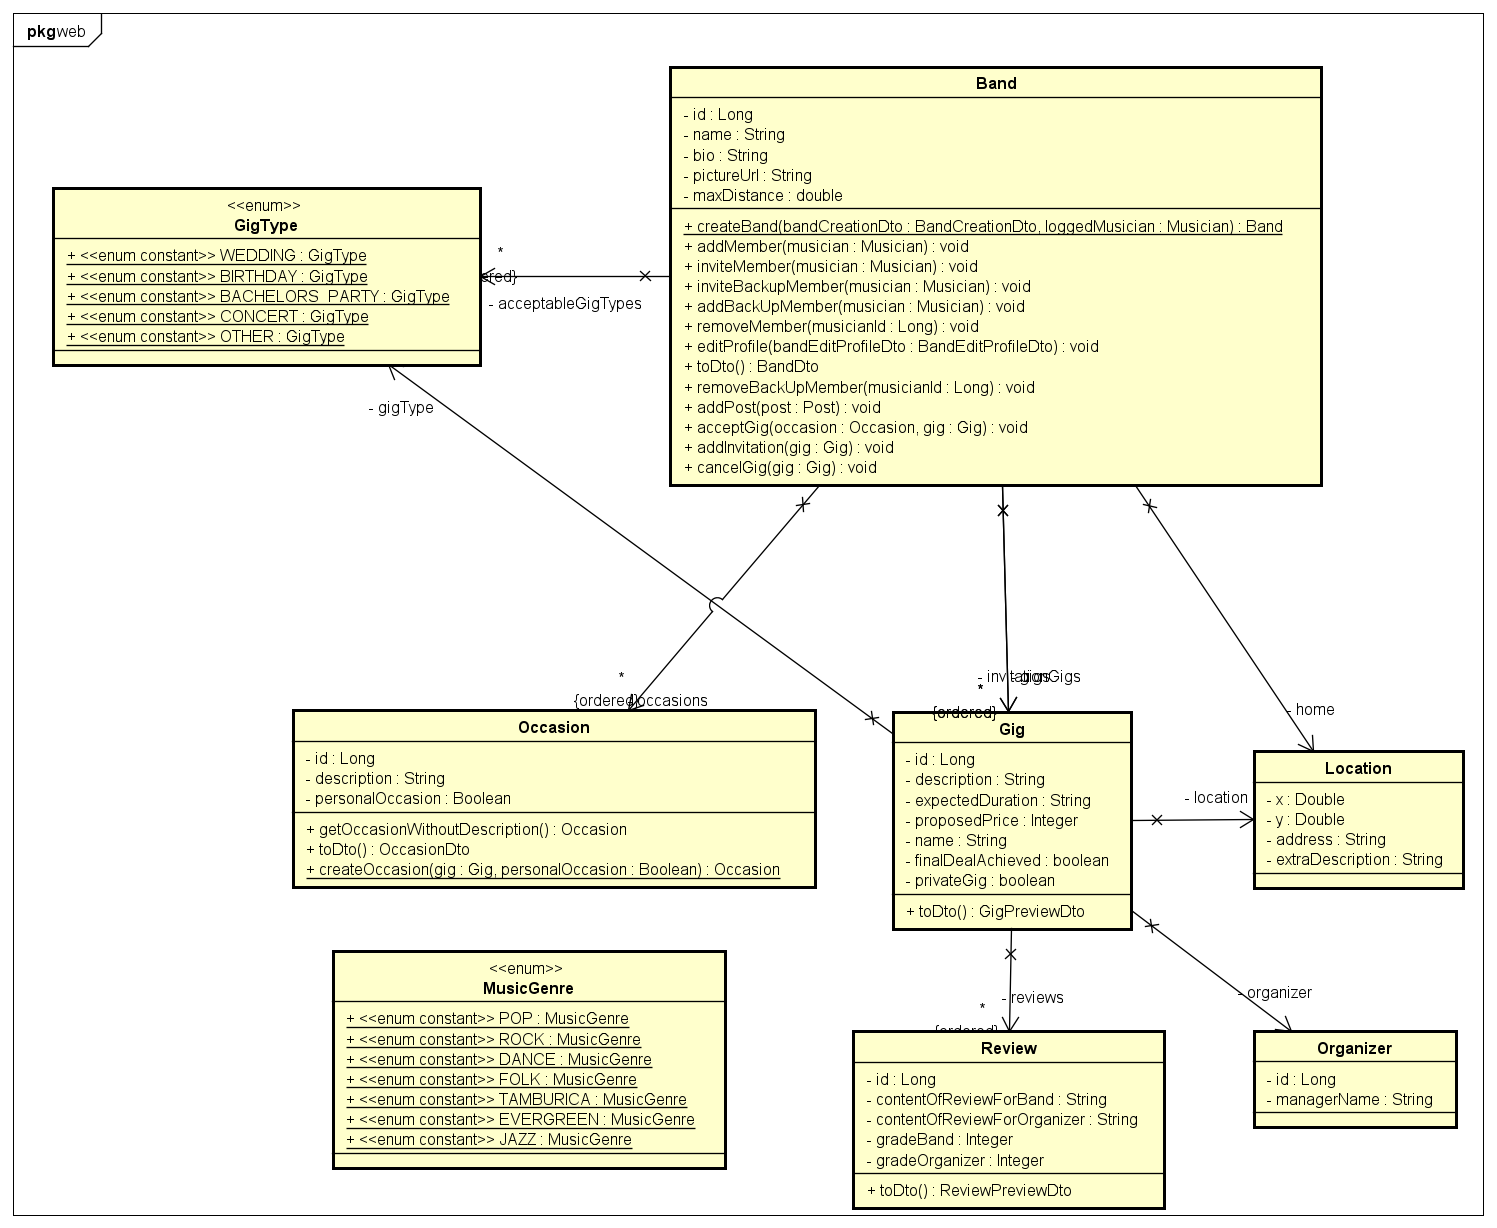
\includegraphics[width=17cm]{slike/entiteti_1.PNG}
			\end{center}
			\caption{Dijagram razreda - razredi entiteta 1}
			\label{fig:domena}
		\end{figure}
	
		\begin{figure}[H]
		\begin{center}
			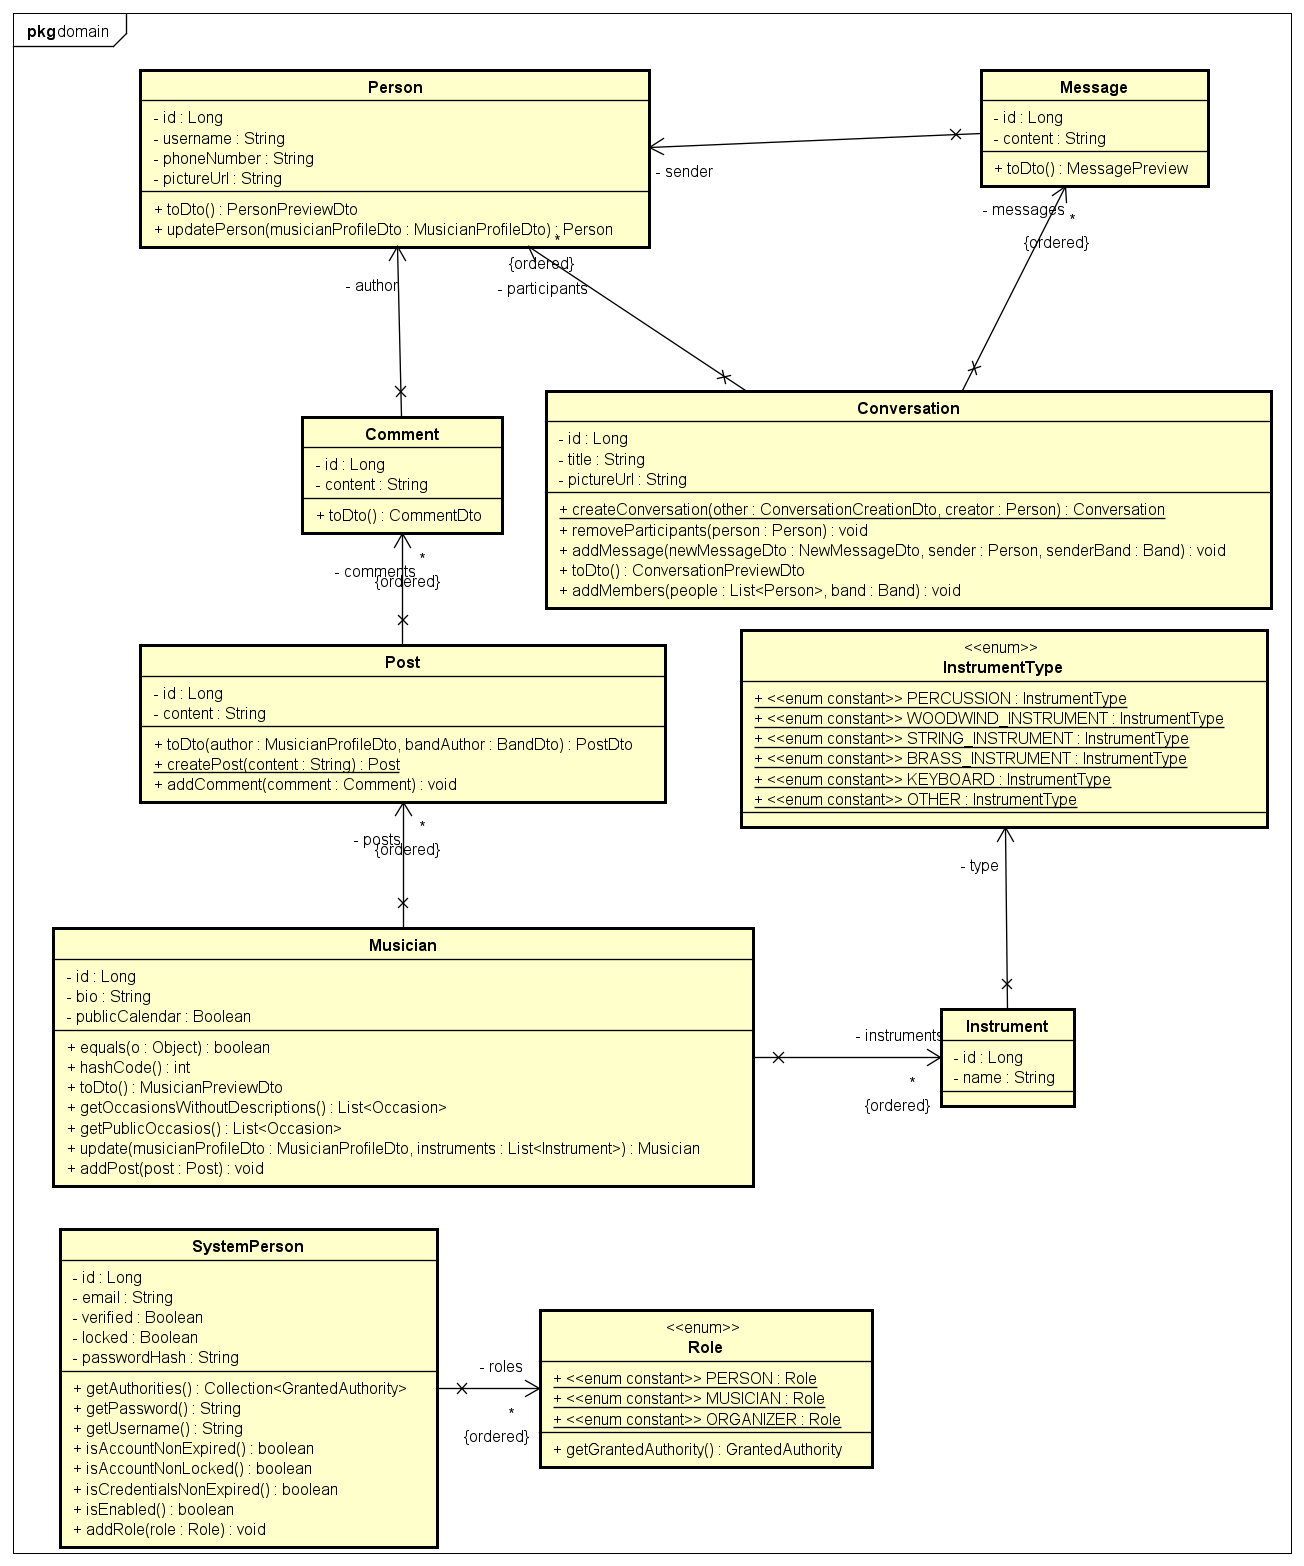
\includegraphics[width=17cm]{slike/entiteti_2.PNG}
		\end{center}
		\caption{Dijagram razreda - razredi entiteta 2}
		\label{fig:domena2}
	\end{figure}
	
	Na slici 4.7 prikazan je dijagram razreda zaduženih za Spring Security.
	Ulazna točka za autorizaciju zahtjeva je definirana u JwtRequestFilteru koji poziva UserDetailsServiceImpl da provjeri postoji li u bazi podataka zapis s akreditacijama koje se dekodiraju iz jwt tokena.
	AuthenticateController je zadužen za pružanje jwt tokena ukoliko u bazi pronađe zapis s odgovarajućim vrijednostima.
	Aplikacija ne pamti sesiju niti stanje (STATELESS) tako da korisnik prilikom postavljanja zahtjeva mora dostaviti svoj jwt token putem kojeg se autentificira i autorizira.
	JwtUtil klasa je puna pomoćnih metoda za baratanje jwt tokenom, a UserDetailsServiceImpl je posrednik između baze korisnika i AuthenticateControllera.
	Vezano uz autorizaciju, modelirana su tri DTO objekta koji definiraju objekte koje backend prima i daje kao zahtjev ili odgovor.
	

		\begin{figure}[H]
			\begin{center}
				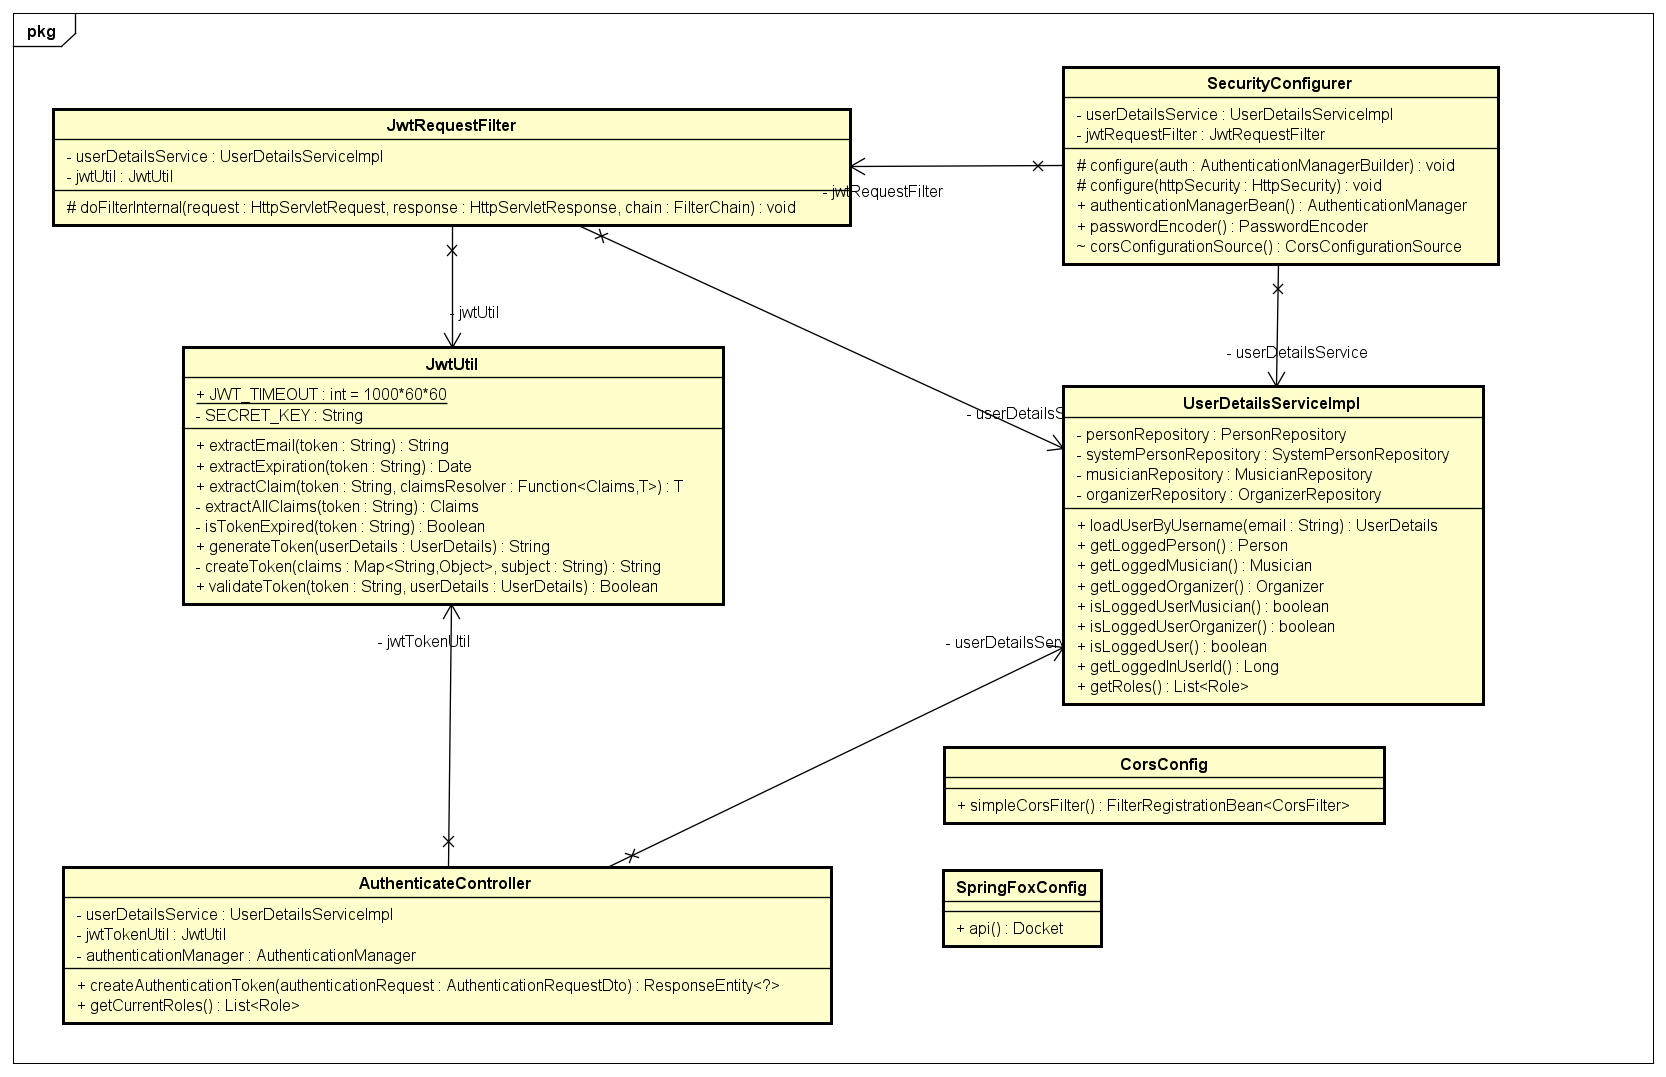
\includegraphics[width=17cm]{slike/security1.PNG}
			\end{center}
			\caption{Dijagram razreda - security}
			\label{fig:sec}
		\end{figure}
	
	Za dohvat podataka iz baze podataka koristimo Jakarta Persistence. Jakarta persistence je specifikacija programskog sučelja Java aplikacije koja opisuje upravljanje relacijskim podacima u aplikaciji. U ovoj aplikaciji za svaki entitet definiran je zasebni repozitorij koji nasljeđuje JpaRepositoryj. Jpa Repository sadrži osnovne metode za dohvat podataka, a Spring Boot omogućuje programeru da specificiranjem samo imena metode dobije implementaciju iste na korištenje. 
	
		\begin{figure}[H]
			\begin{center}
				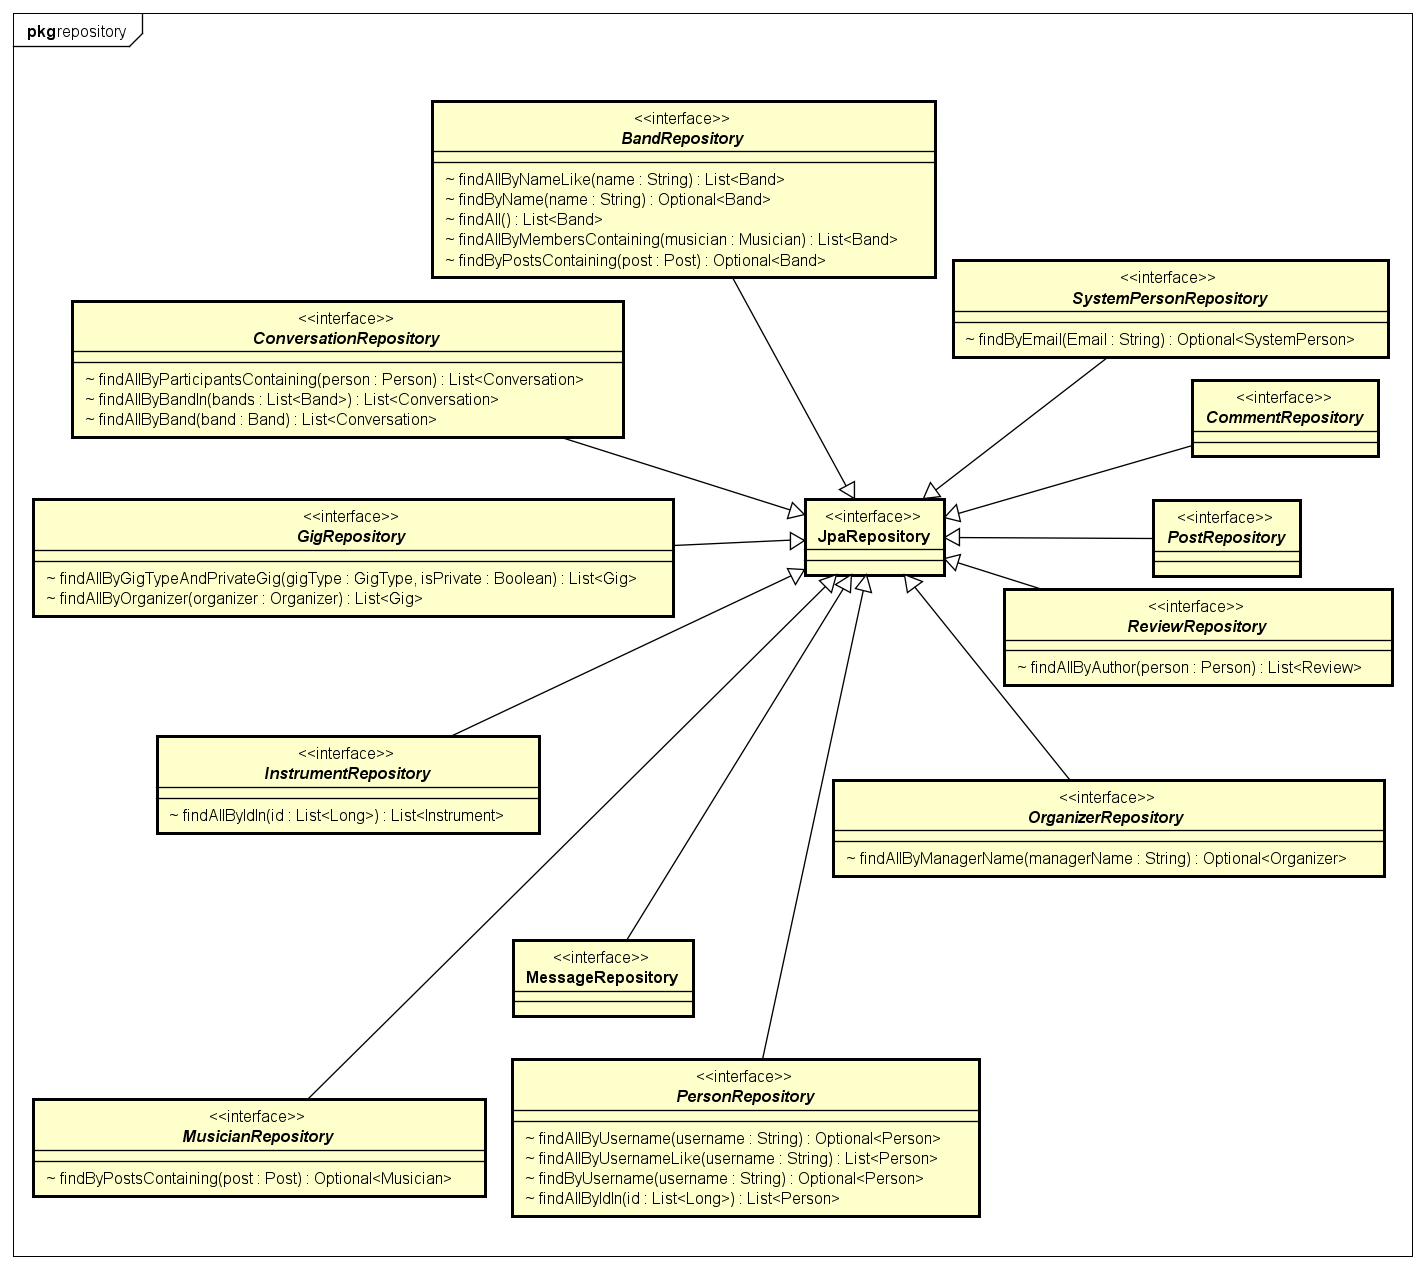
\includegraphics[width=17cm]{slike/repository1.PNG}
			\end{center}
			\caption{Dijagram repozitorija - repository}
			\label{fig:repository}
		\end{figure}
	
	Ovim dijagramom prikazane su moguće pogreške kao i iznimke. Pogreške se u ovom slučaju nalaze u Enumu Errorcode i služe za zaustavljanje operacija čijim izvođenjem se krši pravo pristupa ili se pokušava izvesti nemoguća akcija. Sve ostale logičke iznimke omotavaju se u iznimu GigerException. Za reprezentacijsko stanje prijenosa uvedena je iznimka RestExceptionHandler.
		
		\begin{figure}[H]
			\begin{center}
				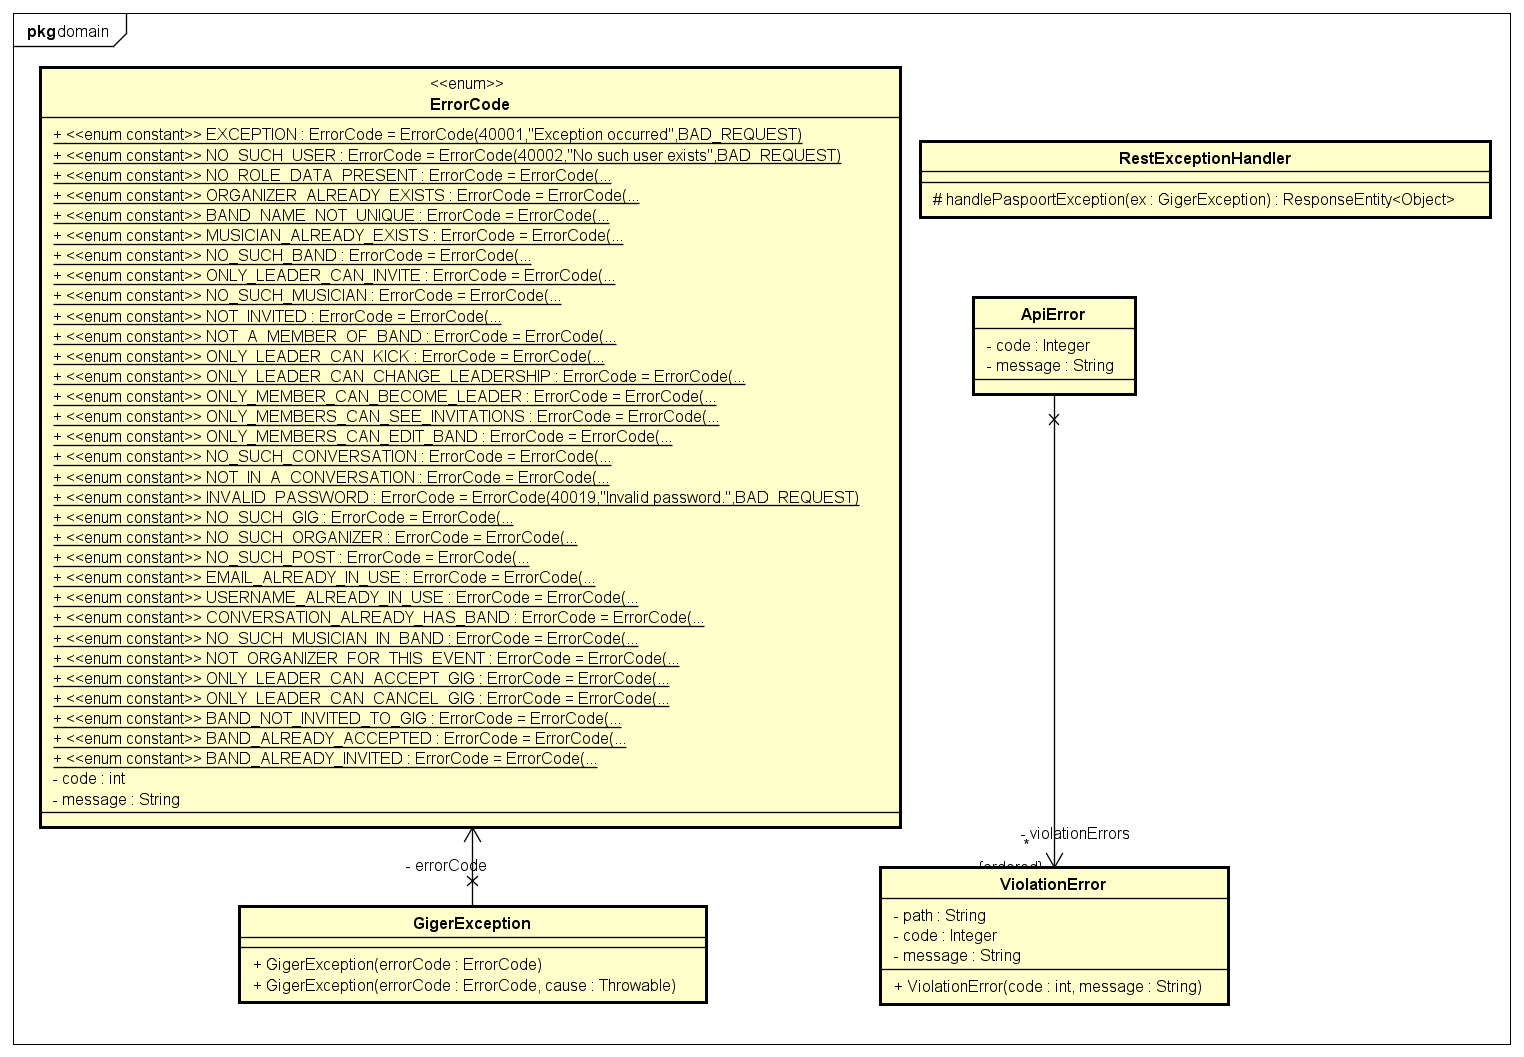
\includegraphics[width=17cm]{slike/errors1.PNG}
			\end{center}
			\caption{Dijagram razreda - errors}
			\label{fig:err}
		\end{figure}
	
		
	
	
	\eject
	
	\section{Dijagram stanja}
	
    Sljedeći dijagram stanja prikazuje stvaranje giga.Nakon uspješnog stvaranja giga, isti i dalje nije viđen pod opcijom "View public gigs". Da bi ostali korisnici mogli vidjeti taj gig, on prvo mora biti finaliziran.To znači da  organizator mora pozvati bend u svoj gig te nakon  što bend prihvati nastup ,gig postaje finaliziran (javan).
	
	
	
	
		\begin{figure}[H]
			\begin{center}
				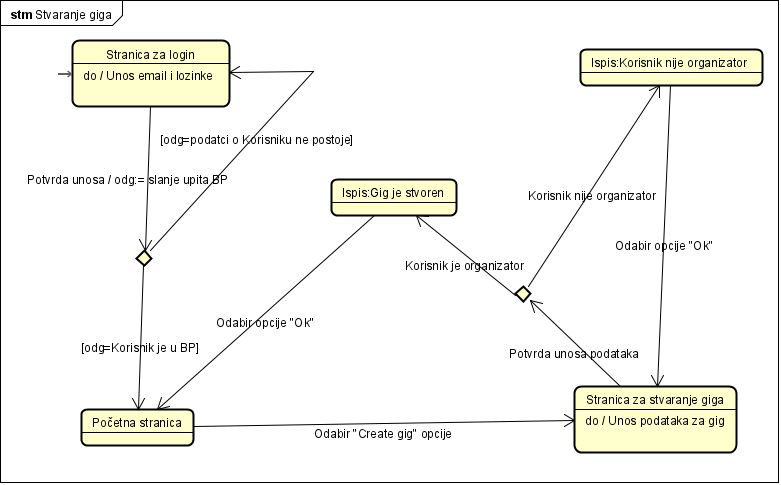
\includegraphics[width=17cm]{slike/stmStvaranjGiga.JPG}
			\end{center}
			\caption{Dijagram stanja - stvaranje giga}
			\label{fig:stm}
		\end{figure}
	
	\eject
	
	
	\section{Dijagram aktivnosti}
	
	\textit{\textbf{dio 2. revizije}} \\
	
	\textit{Potrebno je priložiti dijagram aktivnosti s pripadajućim opisom. Dijagram aktivnosti treba prikazivati značajan dio sustava.} \\
	
	
	\eject
	
	
	
	\section{Dijagram komponenti}
	
	\textit{\textbf{dio 2. revizije}} \\
	
	\textit{Potrebno je priložiti dijagram komponenti s pripadajućim opisom. Dijagram komponenti treba prikazivati strukturu cijele aplikacije.} \\
	
	\eject	

	\chapter{Implementacija i korisničko sučelje}
		
		
		\section{Korištene tehnologije i alati}
		
			\textbf{\textit{dio 2. revizije}} \\
			
			 \textit{Detaljno navesti sve tehnologije i alate koji su primijenjeni pri izradi dokumentacije i aplikacije. Ukratko ih opisati, te navesti njihovo značenje i mjesto primjene. Za svaki navedeni alat i tehnologiju je potrebno \textbf{navesti internet poveznicu} gdje se mogu preuzeti ili više saznati o njima}.
			

    	
        \begin{longtabu} to \textwidth {|X[6, l+3]|X[25, 1]|X[20, 2]|}
		
    		\hline \multicolumn{3}{|c|}{\textbf{Backend}}	 \\[3pt] \hline
    		\endfirsthead
    		
    		\hline
    		\endlastfoot
    		
    		PostgreSQL & \href{https://www.postgresql.org/}{https://www.postgresql.org/}	& Objektno-relacijska baza podataka 	\\ \hline
    		Java 11 & \href{https://www.oracle.com/technetwork/java/javase/downloads/jdk11-downloads-5066655.html}{https://www.oracle.com} & Programski jezik u kojem je napisan backend dio aplikacije	\\ \hline
    		Java Spring Boot & \href{https://spring.io/projects/spring-boot}{https://spring.io/projects/spring-boot} & Razvojni okvir 	\\ \hline
    		
    		Spring Web MVC  & \href{https://docs.spring.io/spring/docs/current/spring-framework-reference/web.html}{https://docs.spring.io/spring/} & Web framework za rukovanje zahtjevima 	\\ \hline
    		Spring Security  & \href{https://spring.io/projects/spring-security}{https://spring.io/projects/spring-security} & 
Moćan i vrlo prilagodljiv okvir za provjeru autentičnosti i kontrolu pristupa 	\\ \hline

        Lombok  & \href{https://projectlombok.org/}{https://projectlombok.org/} & Java library za pregledniji kod 	\\ \hline
    	\end{longtabu}
			
			

			\eject
			
        \begin{longtabu} to \textwidth {|X[4, l+3]|X[25, l]|X[20, 2]|}
		
    		\hline \multicolumn{3}{|c|}{\textbf{Frontend}}	 \\[3pt] \hline
    		\endfirsthead
    		
    		\hline
    		\endlastfoot
    		
    		React & \href{https://reactjs.org/}{https://reactjs.org/}	& JavaScript library za izgradnju sučelja	\\ \hline
    		Ant Design & \href{https://ant.design/}{https://ant.design/} & Design library sa komponentama za lakšu izgradnju korisničkog sučelja	\\ \hline
    		
    		NPM & \href{https://www.npmjs.com/}{https://www.npmjs.com/} & Upravitelj paketa za programski jezik JavasScript	\\ \hline
    		
    		OpenCage Geocoder & \href{https://opencagedata.com/}{https://opencagedata.com/} & API za dohvaćanje koordinata iz adrese	\\ \hline
    	\end{longtabu}			
			
			
        \begin{longtabu} to \textwidth {|X[4, l+3]|X[25, l]|X[20, 2]|}
		
    		\hline \multicolumn{3}{|c|}{\textbf{Komunikacija}}	 \\[3pt] \hline
    		\endfirsthead
    		
    		\hline
    		\endlastfoot
    		
    		Slack & \href{https://slack.com/intl/en-hr/}{https://slack.com/intl/en-hr/}	& Platforma koju smo koristili za lakšu komunikaciju	\\ \hline
    		Trello & \href{https://trello.com/en}{https://trello.com/en} & Alat koji nam je olakšao zajedniči rad i raspoređivanje  projektnih zadataka	\\ \hline
    	\end{longtabu}
    
        \eject
			
			
			
		
	
		\section{Ispitivanje programskog rješenja}
	
			
			\subsection{Ispitivanje komponenti}
			\textit{Potrebno je provesti ispitivanje jedinica (engl. unit testing) nad razredima koji implementiraju temeljne funkcionalnosti. Razraditi \textbf{minimalno 6 ispitnih slučajeva} u kojima će se ispitati redovni slučajevi, rubni uvjeti te izazivanje pogreške (engl. exception throwing). Poželjno je stvoriti i ispitni slučaj koji koristi funkcionalnosti koje nisu implementirane. Potrebno je priložiti izvorni kôd svih ispitnih slučajeva te prikaz rezultata izvođenja ispita u razvojnom okruženju (prolaz/pad ispita). }
			
			
			
			Da bismo testirali backend, napravili smo dvije vrste testova. JUnit testove za testiranje servisa te integracijske testove koje je najlakše opisati kao automatizirane Postman zahtjeve.
			
			Servisi su testirani na način da ih gledamo kao crne kutije koje za određeni ulaz trebaju odraditi određene akcije ili vratiti određene objekte. Nomenklatura testovi servisa (BandServiceTest) slijedi pravilo given\_when\_then. Naprimjer, ako testiramo metodu naziva createMusician, pretpostavljajuci da on još ne postoji i očekujući da se kreira glazbenik u bazi, naziv testa bio bi 
			noSuchMusician\_
			createMusician\_createAndPersistateMusician().
			
			Pomoću Mockito frameworka u testovima mockamo (oponašamo) ulaze te na taj način kontroliramo ulaze i okolinu metode koju testiramo. Drugim riječima, kada radimo test za neku komponentu ili servis, pretpostavljamo da su svi ulazi dobri i ne zanima nas utjecaj naše komponente na drugu komponentu, već samo direktni izlaz. Na taj način dobivamo testove koji su međusobno nepovezani i koji definiraju željeno ponašanje aplikacije. Ukoliko u daljnjem razvoju neki od razvojnih programera promijeni neko ponašanje koje ima utjecaj na druge komponente, pravilno napisani testovi trebali bi pasti i upozoriti ga da će se njegova promjena propagirati dublje u aplikaciju. Testovi koji su pisani ciljano na pojedine komponente sustava u kontroliranim uvjetima prilikom izvođenja precizno ukazuju na vjerojatan izvor pogreške. Na primjer, ako promijenimo implementaciju kreiranja glazbenika te on u trenutku kreiranja ne dobije id, samo testovi koji provjeravaju parametre nakon inicijalizacije bi trebali pasti, a ne svi testovi koji se u nekom trenutku pozivaju na tu funkcionalnost.
			
			Svaki napisan test odijeljen je u tri cjeline, a to su Arrange, Act, Assert. U prvom dijelu uređujemo i mockamo ulaze u testirajuću komponentu, na prije opisan način. U drugom dijelu testa poziva se akcija ili niz akcija čije djelovanje želimo provjeriti, a u trećem dijelu testa provjeravamo jesu li posljedice izvršavanja drugoga dijela testa u skladu s očekivanjima.
			
			Na slici 5.1 nalazi se primjer unit testa. Linije 380-399 su Arrange, linija 401 je Act, dok su linije 404-408 Assert dio testa.
			
			\begin{figure}[H]
				\begin{center}
					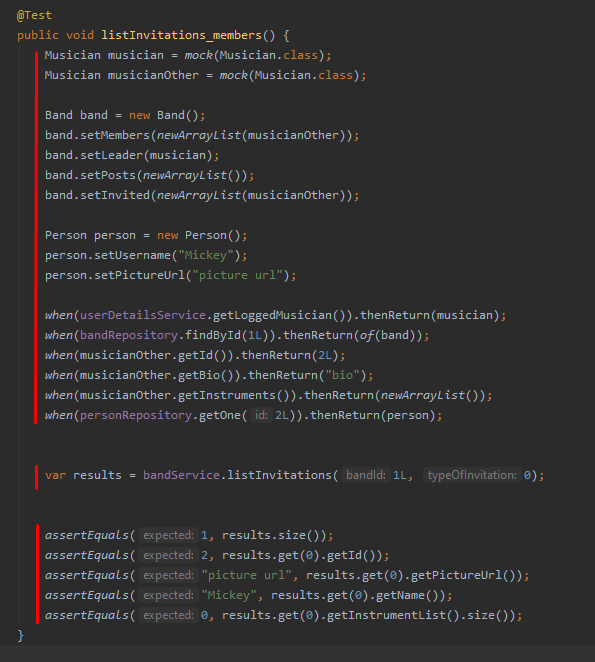
\includegraphics[width=13cm]{slike/junit_test.PNG}
				\end{center}
				\caption{Primjer JUnit testa}
				\label{fig:junit}
			\end{figure}
		
			
			Pošto je pisanje testova često i iscrpnije od pisanja implementacije (BandService ima 210 linija koda, dok BandServiceTest koji ni ne testira baš sve metode u njemu ima 558), za ovaj projekt nismo radili TDD (test driven development) već smo naknadno radili testove za postojeću implementaciju kako bismo potvrdili implementaciju i programski dokumentirali očekivano ponašanje.
			
			Uz dodatak BandService testovima postoji i nekoliko testova u EmailSenderTest koji pokazuju kako testirati komponentu čiju implementaciju ne znamo.
			
			
			Uz tridesetak JUnit testova čija je glavna prednost brzo izvođenje, napisali smo desetak integracijskih testova. Kao što smo već spomenuli, integracijski testovi slični su ručnom pregledavanju u Postmanu. Svaki integracijski test pokreće aplikaciju ispočetka tako da su mu stanje baze i aplikacije (kontekst) jednaki kao kad se pokrene aplikacija. U ovim testovima koristimo MockMvc kako bismo simulirali http request kojemu moramo odrediti metodu (GET, POST) te dodati pripadajuća zaglavlja. U ovom testu verificiramo je li ono što je vratila metoda jednako onome što se očekivalo (najčešće usporedbe DTO-ova).
			
			\begin{figure}[H]
				\begin{center}
					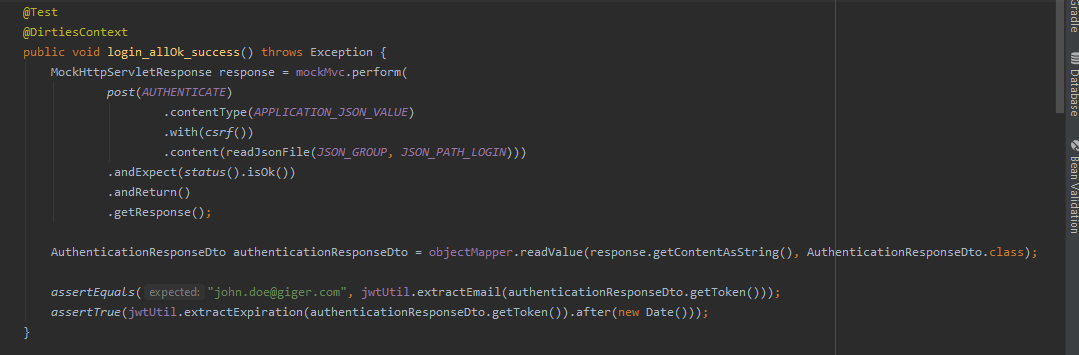
\includegraphics[width=17cm]{slike/integracijski_test.PNG}
				\end{center}
				\caption{Primjer integracijskog testa}
				\label{fig:inttest}
			\end{figure}
			
			Tehnike testiranja programske potpore nadahnute su knjigom Test-Driven Development Kenta Becka.
			
			
			
			\subsection{Ispitivanje sustava}
			
			 \textit{Potrebno je provesti i opisati ispitivanje sustava koristeći radni okvir Selenium\footnote{\url{https://www.seleniumhq.org/}}. Razraditi \textbf{minimalno 4 ispitna slučaja} u kojima će se ispitati redovni slučajevi, rubni uvjeti te poziv funkcionalnosti koja nije implementirana/izaziva pogrešku kako bi se vidjelo na koji način sustav reagira kada nešto nije u potpunosti ostvareno. Ispitni slučaj se treba sastojati od ulaza (npr. korisničko ime i lozinka), očekivanog izlaza ili rezultata, koraka ispitivanja i dobivenog izlaza ili rezultata.\\ }
			 
			 \textit{Izradu ispitnih slučajeva pomoću radnog okvira Selenium moguće je provesti pomoću jednog od sljedeća dva alata:}
			 \begin{itemize}
			 	\item \textit{dodatak za preglednik \textbf{Selenium IDE} - snimanje korisnikovih akcija radi automatskog ponavljanja ispita	}
			 	\item \textit{\textbf{Selenium WebDriver} - podrška za pisanje ispita u jezicima Java, C\#, PHP koristeći posebno programsko sučelje.}
			 \end{itemize}
		 	\textit{Detalji o korištenju alata Selenium bit će prikazani na posebnom predavanju tijekom semestra.}
			
			\eject 
		
		
		\section{Dijagram razmještaja}
			 
			 Dijagrami razmještaja opisuju topologiju sklopovlja i programsku potporu koja se koristi u implementaciji sustava u njegovom radnom okruženju. Sve komponente programske potpore smještene su na oblak platformu Heroku. Heroku kao platforma omogućuje programerima izvođenje i operiranje nad aplikacijama u oblaku. U ovome slučaju pozadinska i prednja aplikacija razmještene su na zasebene poslužitelje kao i baza podataka. Sustav je baziran na arhitekturi klijent - poslužitelj i komunikacija između njih odvija se HTTP protokolom. 
			 
			 	\begin{figure}[H]
			 	\begin{center}
			 		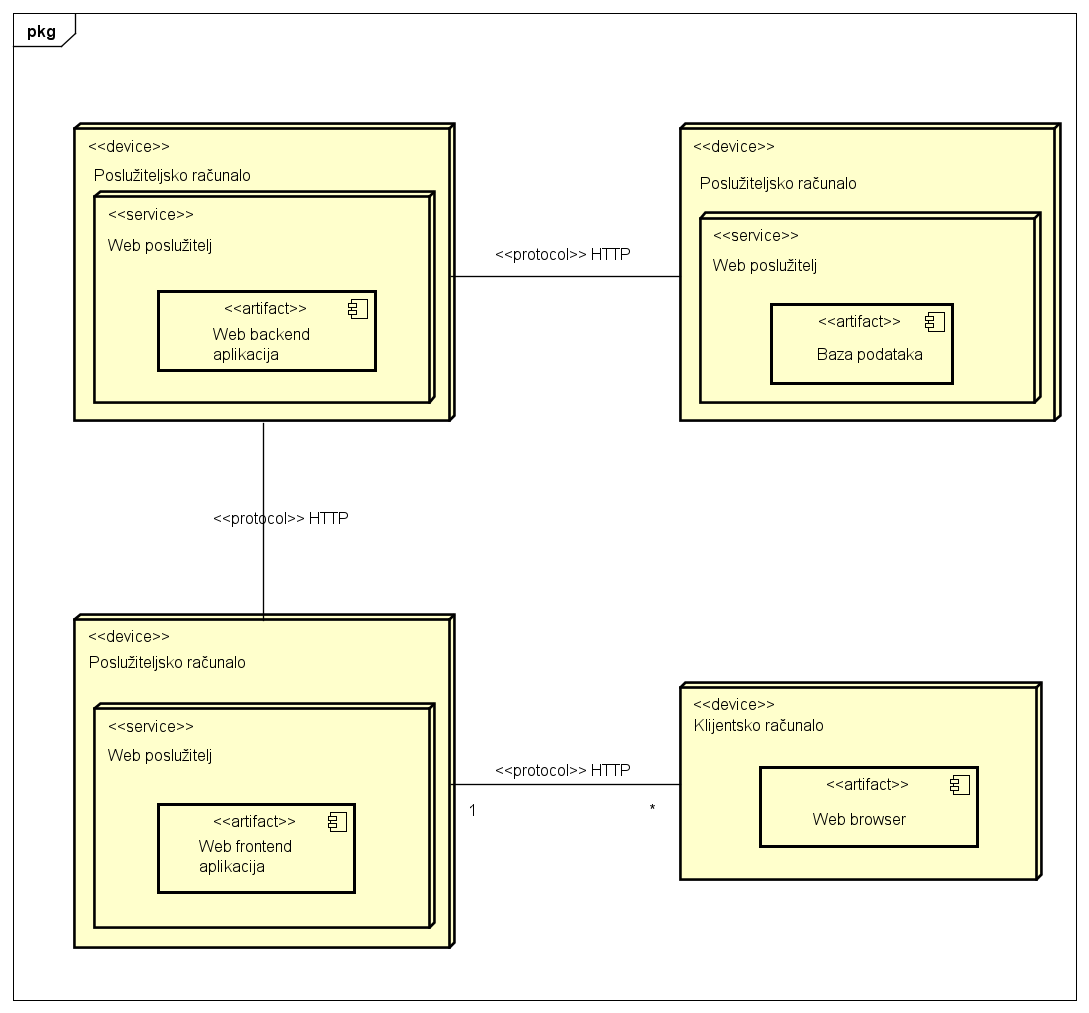
\includegraphics[width=15cm]{slike/deploy_fin.PNG}
			 	\end{center}
			 	\caption{Dijagram razmještaja}
			 	\label{fig:deploy_pic}
			 \end{figure}
			
			\eject 
		
		\section{Upute za puštanje u pogon}
			
			
			Ponajprije je potrebno preuzeti Postgres SQL bazu podataka na operacijski sustav, poželjno Windows. Nakon toga je potrebno provesti standardnu instalaciju. U servisu LoaderService nalaze se testni podaci za inicijalno punjenje baze. Za postavljanje lozinke baze potrebno je je u password polje u system-local.properties postaviti prethodno definiranu lozinku za bazu podataka. Alternativno moguće je u root direktoriju standardnog terminala  pokrenuti naredbu docker-compose up koja će u virtualnom kontejneru pokrenuti servise koji su predefinirani u dockeru docker-compose.yml datoteci. Za konfiguraciju aplikacije na Heroku poslužitelju koristi se system.properties iz kojeg se čita pokretanje Spring Boot aplikacije defaultnim profilom.
			U izradi aplikacije korišten je radni okvir Spring Boot. Za pokretanje Javine aplikacije
			potrebno je imati instaliran Java Runtime Environment v11. Za pokretanje frontend aplikacije
			potrebno je imati instaliranu platformu Node.js. Za pokretanje također je potrebno otpakirati 
			arhivu server.var. Kako bi se pokrenuo build koristi se automatizirani sustav Gradle. 
			
			\eject 
	\label{key}\chapter{Zaključak i budući rad}
		
		\textbf{\textit{dio 2. revizije}}\\
		
		 \textit{U ovom poglavlju potrebno je napisati osvrt na vrijeme izrade projektnog zadatka, koji su tehnički izazovi prepoznati, jesu li riješeni ili kako bi mogli biti riješeni, koja su znanja stečena pri izradi projekta, koja bi znanja bila posebno potrebna za brže i kvalitetnije ostvarenje projekta i koje bi bile perspektive za nastavak rada u projektnoj grupi.}
		
		 \textit{Potrebno je točno popisati funkcionalnosti koje nisu implementirane u ostvarenoj aplikaciji.}
		
		\eject 
		
	
	\chapter*{Popis literature}
		\addcontentsline{toc}{chapter}{Popis literature}
	 	
 		\begin{enumerate}
			
			
			\item  Oblikovanje programske potpore, FER ZEMRIS, \url{http://www.fer.hr/predmet/opp}
			
			\item Astah Community, \url{http://astah.net/editions/uml-new}
			\item GitLab Pipelines, \url{https://docs.gitlab.com/ee/ci/pipelines.html}
			\item Sprint Boot, \url{https://docs.spring.io/spring-boot/docs/current-SNAPSHOT/reference/htmlsingle/}
			\item Kent Beck, \textit{Test Driven Development}, 2000.
		\end{enumerate}
		
		 
	
	
	\begingroup
	\renewcommand*\listfigurename{Indeks slika i dijagrama}
	%\renewcommand*\listtablename{Indeks tablica}
	%\let\clearpage\relax
	\listoffigures
	%\vspace{10mm}
	%\listoftables
	\endgroup
	\addcontentsline{toc}{chapter}{Indeks slika i dijagrama}


	
	\eject 
		
	\chapter*{Dodatak: Prikaz aktivnosti grupe}
		\addcontentsline{toc}{chapter}{Dodatak: Prikaz aktivnosti grupe}
		
		\section*{Dnevnik sastajanja}
		
		\begin{packed_enum}
			\item  sastanak
			
			\item[] \begin{packed_item}
				\item Datum: 3. listopada 2019.
				\item Prisutni: I. Juren, T. Krmek, M. Jurić, M. Zec, S. Gaši, M. Nosil, P. Lanča
				\item Teme sastanka:
				\begin{packed_item}
					\item  predlaganje ideja za projektni zadatak
					\item  odabir između web ili mobilne aplikacije
					\item  svaki član je iznio koja predznanja ili iskustva ima vezano za stvaranje aplikacije  
				\end{packed_item}
			\end{packed_item}
			
			\item  sastanak
			\item[] \begin{packed_item}
				\item Datum: 9. listopada 2019.
				\item Prisutni: I. Juren, T. Krmek, M. Jurić, M. Zec, S. Gaši, M. Nosil, P. Lanča
				\item Teme sastanka:
				\begin{packed_item}
					\item  upoznavanje s mentorima i demonstratorom
					\item  razgovor o tehnologijama koje ćemo koristiti
					\item  dogovoren način komunikacije s asistentom i demonstratorom
					\item  upoznavanje s ponuđenim projektom te razgovor o tome kako poboljšati naš prijedlog projekta
				\end{packed_item}
			\end{packed_item}
			
			\item  sastanak
			\item[] \begin{packed_item}
				\item Datum: 14. listopada 2019.
				\item Prisutni: I. Juren, M. Jurić, M. Zec, S. Gaši, P. Lanča
				\item Teme sastanka:
				\begin{packed_item}
					\item  sastanak s asistentom
					\item  nacrtana gruba shema različitih korisnika s pripadajućim potrebnim pristupom
					\item  predlaganje funkcionalnosti, dogovoreno što se obavezno mora implementirati 
				\end{packed_item}
			\end{packed_item}
			
			\item  sastanak
			\item[] \begin{packed_item}
				\item Datum: 22. listopada 2019.
				\item Prisutni: I. Juren, T. Krmek, M. Jurić, M. Zec, S. Gaši, M. Nosil, P. Lanča
				\item Teme sastanka:
				\begin{packed_item}
					\item  razrada must i could have funkcionalnosti
					\item  izjašnjavanje svojih nedoumica te njihovo razrješavanje, eventualno stavljene na popis za pitanja na sastanku s asistentom
					\item  razriješena problematika benda (glavni i rezervni članovi)
					\item  nakon internog, sastanak s asistentom: dogovorena detaljnija implementacija, napravljen popis zadataka koje treba odraditi do idućeg sastanka
				\end{packed_item}
			\end{packed_item}
			
			\item  sastanak
			\item[] \begin{packed_item}
				\item Datum: 28. listopada 2019.
				\item Prisutni: I. Juren, M. Jurić, M. Zec, S. Gaši, M. Nosil, P. Lanča
				\item Teme sastanka:
				\begin{packed_item}
					\item  nabrajanje usecase-ova
					\item  podjela rada
					\item  određena pitanja za idući sastanak s asistentom
				\end{packed_item}
			\end{packed_item}
			
			\item  sastanak
			\item[] \begin{packed_item}
				\item Datum: 29. listopada 2019.
				\item Prisutni: I. Juren, M. Jurić, M. Zec, S. Gaši, M. Nosil, P. Lanča
				\item Teme sastanka:
				\begin{packed_item}
					\item  sastanak s asistentom: pokazano što je sve napravljeno
					\item  napravljen popis zadataka koji moraju biti gotovi do idućeg sastanka s asistentom i sve što još treba za prvu verziju
					\item  riješena dilema oko recenzija
					\item  razriješen problem solista, bit će jednočlani bend
					\item  rasprava oko baze podataka, što treba promijeniti i poboljšati
				\end{packed_item}
			\end{packed_item}
			
			\item  sastanak
			\item[] \begin{packed_item}
				\item Datum: 11. studenog 2019.
				\item Prisutni: I. Juren, M. Jurić, M. Zec, S. Gaši, M. Nosil, P. Lanča, T. Krmek
				\item Teme sastanka:
				\begin{packed_item}
					\item  određivanje preostalih poslova te njihov raspored po članovima
					\item  na sastanku dovršen frontend te je aplikacija isporučena
				\end{packed_item}
			\end{packed_item}
			
			\item  sastanak
			\item[] \begin{packed_item}
				\item Datum: 12. listopada 2019.
				\item Prisutni: I. Juren, M. Jurić, M. Zec, S. Gaši, M. Nosil, P. Lanča, T. Krmek
				\item Teme sastanka:
				\begin{packed_item}
					\item  sastanak s asistentom: pokazana aplikacija te dokumentacija
					\item  razriješene neke nedoumice oko baze podataka
				\end{packed_item}
			\end{packed_item}
			
			%
			
		\end{packed_enum}
		
		\eject
		\section*{Tablica aktivnosti}
			\begin{longtabu} to \textwidth {|X[7, l]|X[1, c]|X[1, c]|X[1, c]|X[1, c]|X[1, c]|X[1, c]|X[1, c]|}
								
				\cline{2-8} \multicolumn{1}{c|}{\textbf{}} &     \multicolumn{1}{c|}{\rotatebox{90}{\textbf{Ivan Juren }}} & \multicolumn{1}{c|}{\rotatebox{90}{\textbf{Stela Gaši }}} &	\multicolumn{1}{c|}{\rotatebox{90}{\textbf{Marin Jurić }}} &	\multicolumn{1}{c|}{\rotatebox{90}{\textbf{Tomislav Krmek   }}} &
				\multicolumn{1}{c|}{\rotatebox{90}{\textbf{Paolo Lanča }}} &
				\multicolumn{1}{c|}{\rotatebox{90}{\textbf{Mihael Nosil }}} &	\multicolumn{1}{c|}{\rotatebox{90}{\textbf{Mario Zec }}} \\ \hline 
				\endfirsthead
				
			
				\cline{2-8} \multicolumn{1}{c|}{\textbf{}} &     \multicolumn{1}{c|}{\rotatebox{90}{\textbf{Ivan Juren}}} & \multicolumn{1}{c|}{\rotatebox{90}{\textbf{Stela Gaši }}} &	\multicolumn{1}{c|}{\rotatebox{90}{\textbf{Marin Jurić }}} &
\multicolumn{1}{c|}{\rotatebox{90}{\textbf{Tomislav Krmek }}} &	\multicolumn{1}{c|}{\rotatebox{90}{\textbf{Paolo Lanča }}} &
\multicolumn{1}{c|}{\rotatebox{90}{\textbf{Mihael Nosil }}} &	\multicolumn{1}{c|}{\rotatebox{90}{\textbf{Mario Zec }}} \\ \hline 
				\endhead
				
				
				\endfoot
							
				 
				\endlastfoot
				
				Upravljanje projektom 		& 2 & 1 &  & 1 &  &  & 1 \\ \hline
				Opis projektnog zadatka 	& 3 & 2 &  &  &  &  & \\ \hline
				
				Funkcionalni zahtjevi       & 1 & 2 &  &  &  & 1 & 2 \\ \hline
				Opis pojedinih obrazaca 	&  & 2 & 1 &  & 2 & 10 & 4 \\ \hline
				Dijagram obrazaca 			&  &  &  &  & 1 &  & 3 \\ \hline
				Sekvencijski dijagrami 		&  & 2 & 2 &  & 1 &  &  \\ \hline
				Opis ostalih zahtjeva 		&  &  & 1 &  & 1 &  &  \\ \hline

				Arhitektura i dizajn sustava	 & 3 &  &  &  & 2 &  &  \\ \hline
				Baza podataka				& 6 & 5 &  & 3 &  &  &   \\ \hline
				Dijagram razreda 			& 2 & 1 &  &  &  &  & 5  \\ \hline
				Dnevnik sastajanja 			& 1 & 1 &  &  & 3 &  &  \\ \hline
				Popis literature 			& 1 &  &  &  &  &  &  \\  \hline
				\textit{Frontend} 			& 1 &  & 2 & 15 &  & 2 &  \\ \hline
				\textit{Backend} 				& 20 &  &  &  &  &  &  \\ \hline 
				\textit{Vrijeme provedeno na sastancima} 		 			& 10 & 10 & 10 & 7 & 10 & 9 & 10 \\ \hline 

				
				
			\end{longtabu}
					
					
		\eject
		
		\section*{Dijagrami pregleda promjena}
		
		\begin{figure}[H]
			\begin{center}
				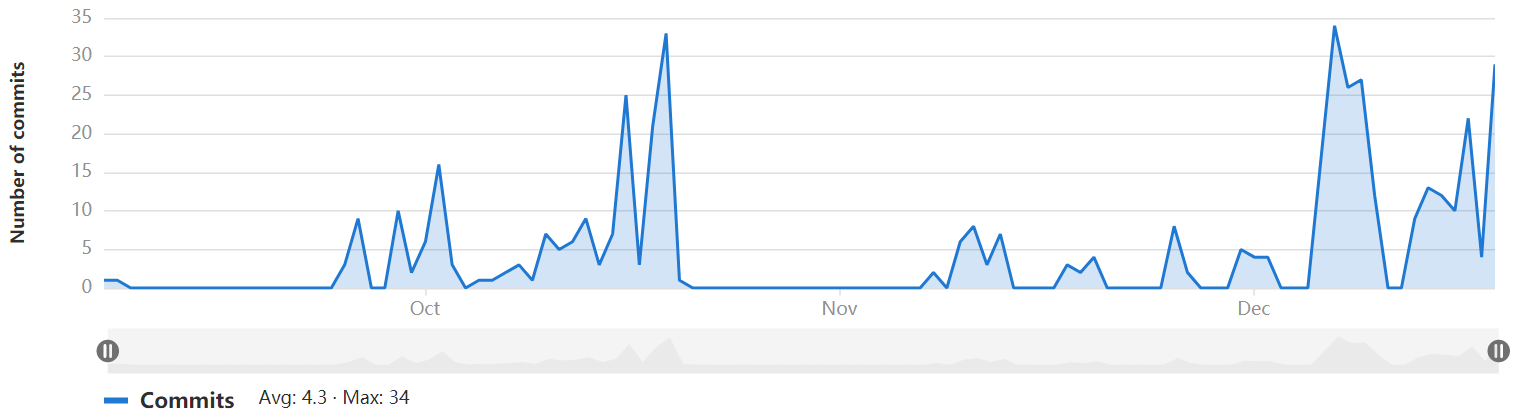
\includegraphics[width=15cm]{slike/dijagrampregledapromjena.PNG}
			\end{center}
			\caption{Dijagram pregleda promjena na grani Master}
			\label{fig:master}
		\end{figure}
		
		\begin{figure}[H]
			\begin{center}
				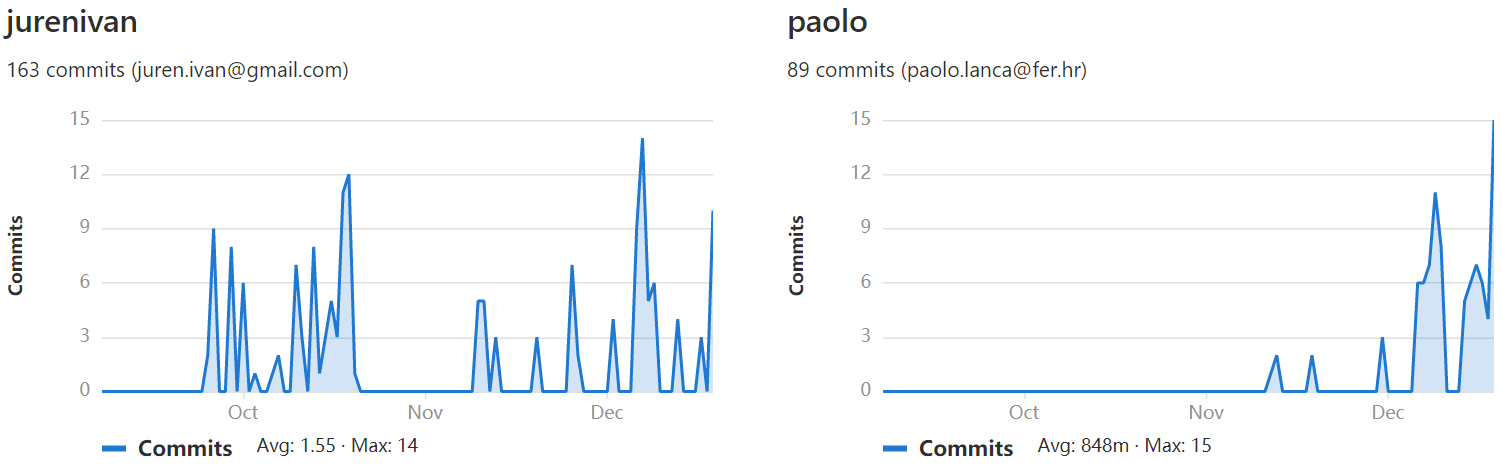
\includegraphics[width=15cm]{slike/dijagrampregledapromjena1.PNG}
				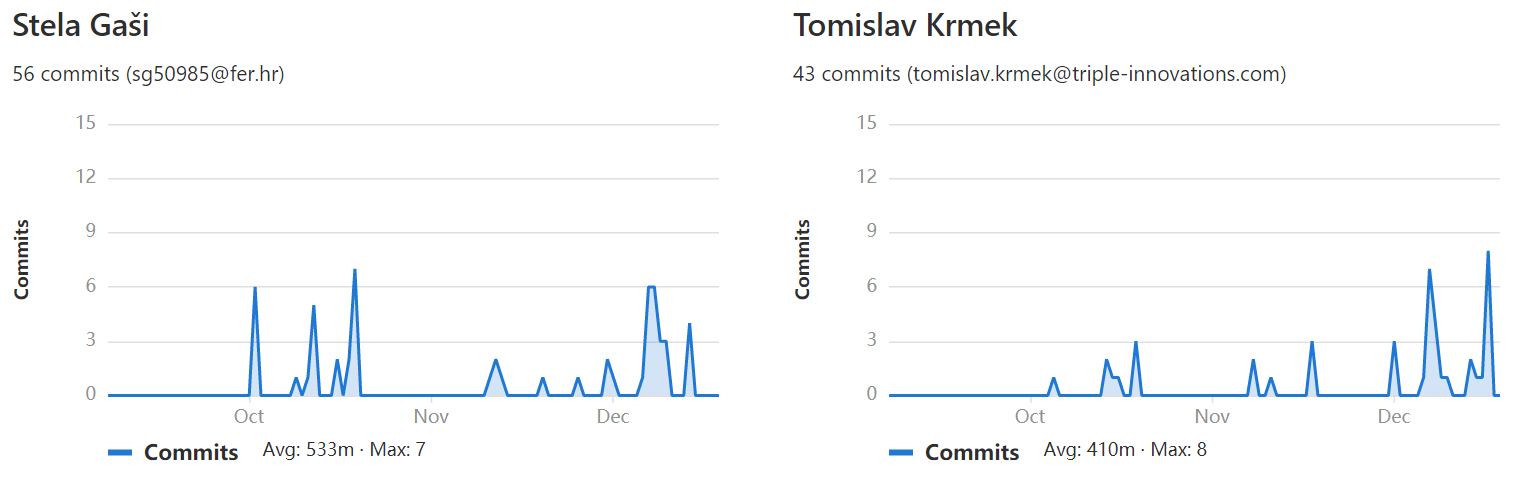
\includegraphics[width=15cm]{slike/dijagrampregledapromjena2.PNG}
				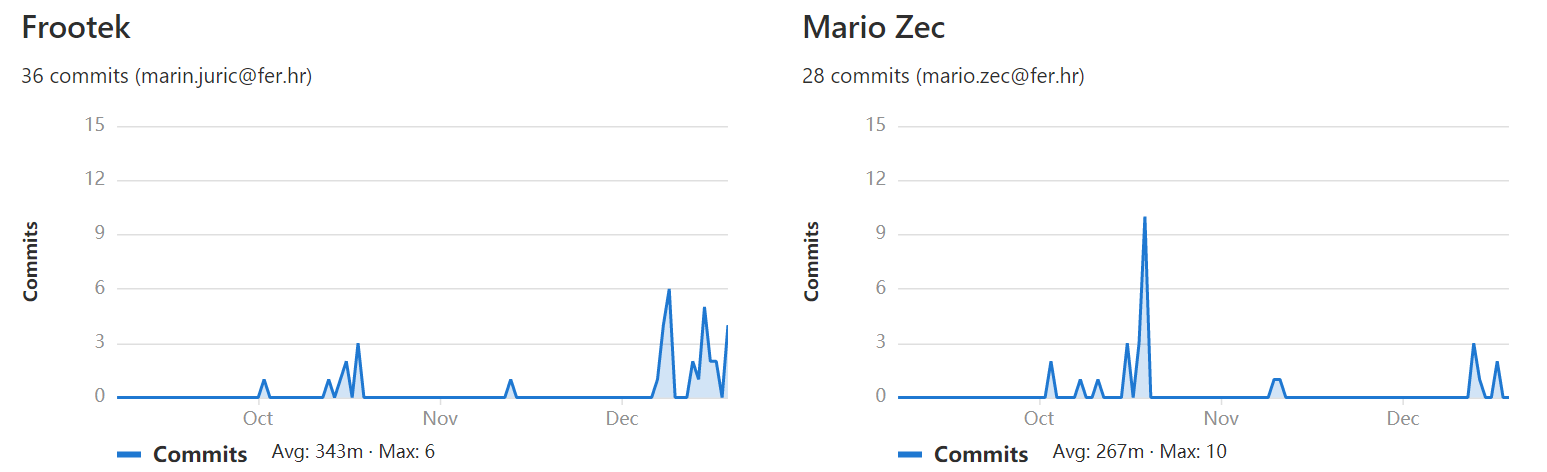
\includegraphics[width=15cm]{slike/dijagrampregledapromjena3.PNG}
				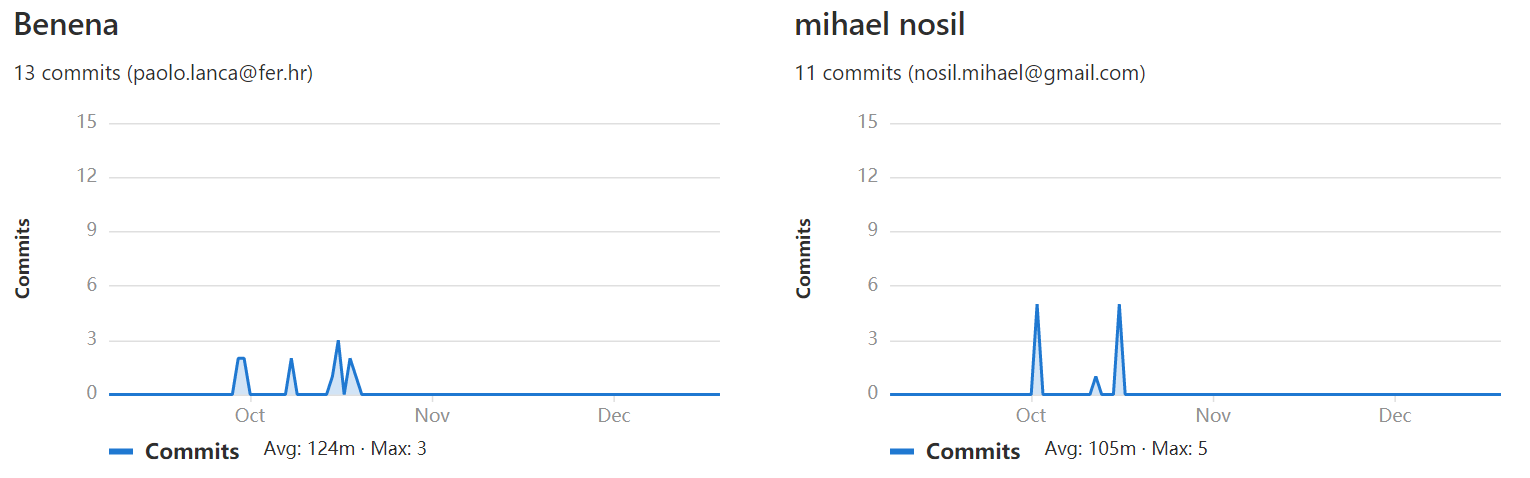
\includegraphics[width=15cm]{slike/dijagrampregledapromjena4.PNG}
				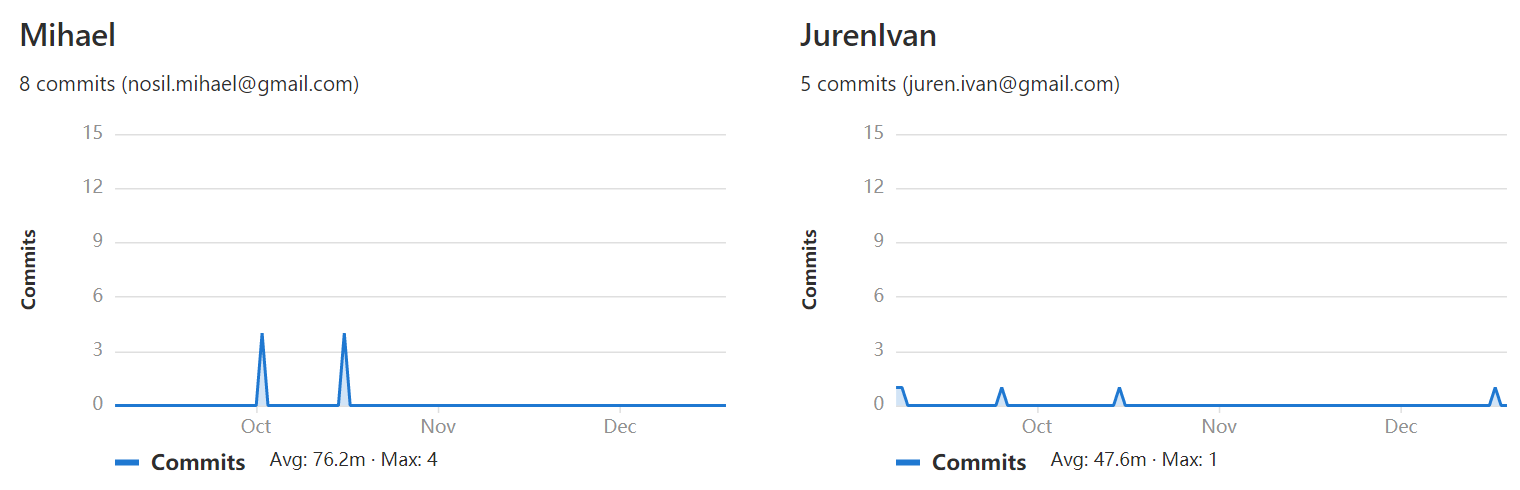
\includegraphics[width=15cm]{slike/dijagrampregledapromjena5.PNG}
			\end{center}
			\label{fig:dijapre}
		\end{figure}



=======

\documentclass[12pt]{report} 

\usepackage[croatian]{babel} 
\usepackage{amssymb}
\usepackage{amsmath}
\usepackage{txfonts}
\usepackage{mathdots}
\usepackage{titlesec}
\usepackage{array}
\usepackage{lastpage}
\usepackage{etoolbox}
\usepackage{longtable, tabu}
\usepackage{color, colortbl}
\usepackage{adjustbox}
\usepackage{geometry}
\usepackage[classicReIm]{kpfonts}
\usepackage{hyperref}
\usepackage{fancyhdr}

\usepackage{float}
\usepackage{setspace}
\restylefloat{table}


\patchcmd{\chapter}{\thispagestyle{plain}}{\thispagestyle{fancy}}{}{}


\titleformat{\chapter}{\normalfont\huge\bfseries}{\thechapter.}{20pt}{\Huge}
\titlespacing{\chapter}{0pt}{0pt}{40pt}
\linespread{1.3}

\geometry{
	a4paper,
	left=1in,
	top=1in,
}

\hypersetup{ colorlinks, citecolor=black, filecolor=black, linkcolor=black,	urlcolor=black }


\newenvironment{packed_enum}{
	\begin{enumerate}
		\setlength{\itemsep}{0pt}
		\setlength{\parskip}{0pt}
		\setlength{\parsep}{0pt}
	}{\end{enumerate}}

\newenvironment{packed_item}{
	\begin{itemize}
		\setlength{\itemsep}{0pt}
		\setlength{\parskip}{0pt}
		\setlength{\parsep}{0pt}
	}{\end{itemize}}


\definecolor{LightBlue}{rgb}{0.9,0.9,1}
\definecolor{LightGreen}{rgb}{0.9,1,0.9}


%podesavanje headera i footera


\pagestyle{fancy}
\lhead{Oblikovanje programske potpore}
\rhead{Giger}
\lfoot{ChillCrew}
\cfoot{stranica \thepage/\pageref{LastPage}}
\rfoot{\today}
\renewcommand{\headrulewidth}{0.2pt}
\renewcommand{\footrulewidth}{0.2pt}


\begin{document}
	

	\begin{titlepage}
		\begin{center}
			\vspace*{\stretch{1.0}}
			\LARGE Oblikovanje programske potpore\\
			\large Ak. god. 2019./2020.\\
			
			\vspace*{\stretch{3.0}}
			
			\huge Giger\\
			\Large Dokumentacija, Rev. \textit{1}\\
			
			\vspace*{\stretch{12.0}}
			\normalsize
			Grupa: \textit{ChillCrew}\\
			Voditelj: \textit{Ivan Juren}\\
			
			
			\vspace*{\stretch{1.0}}
			Datum predaje: \textit{$<$dan$>$. $<$mjesec$>$. $<$godina$>$.}\\
	
			\vspace*{\stretch{4.0}}
			
			Nastavnik: \textit{Tomislav Jukić}\\
		
		\end{center}

	
	\end{titlepage}

	
	\tableofcontents

	\chapter{Dnevnik promjena dokumentacije}
		
		\textbf{\textit{Kontinuirano osvježavanje}}\\
				
		
		\begin{longtabu} to \textwidth {|X[2, l]|X[13, l]|X[3, l]|X[3, l]|}
			\hline \multicolumn{1}{|l|}{\textbf{Rev.}}	& \multicolumn{1}{l|}{\textbf{Opis promjene/dodatka}} & \multicolumn{1}{|l|}{\textbf{Autori}} & \multicolumn{1}{l|}{\textbf{Datum}} \\[3pt] \hline
			\endfirsthead
			
			\hline \multicolumn{1}{|l|}{\textbf{Rev.}}	& \multicolumn{1}{l|}{\textbf{Opis promjene/dodatka}} & \multicolumn{1}{|l|}{\textbf{Autori}} & \multicolumn{1}{l|}{\textbf{Datum}} \\[3pt] \hline
			\endhead
			
			\hline 
			\endlastfoot
			
			0.1 & Napravljen predložak, modificirana \newline glavna .tex datoteka.	& Lanča & 26.10.2019. 		\\[3pt] \hline 
			0.2	& Unesen dnevnik sastanaka. & Lanča & 27.10.2019. 	\\[3pt] \hline 
			0.3 & Dodani \textit{Use Case} dijagrami br. 2, 3, 4, 5, 6 & Jurić & 29.10.2019. \\[3pt] \hline
			0.4 & Dodan \textit{Use Case} dijagram br. 9 & Nosil & 29.10.2019. \\[3pt] \hline
			0.5 & Dodani \textit{Use Case} dijagrami br. 10, 11, 12, 13, \newline 17, 18 & Gaši & 29.10.2019. \\[3pt] \hline
			0.6 & Dodani \textit{Use Case} dijagrami br. 1, 7, 8, 14, 15, \newline 16, 19, 20 & Zec & 30.10.2019. \\[3pt] \hline
			0.7 & Dodani funkcionalni zahtjevi & Zec &         04.11.2019. \\[3pt] \hline 
			0.8 & Nadopunjen zapisnik sastanka, dodani ostali zahtjevi & Lanča & 04.11.2019. \\[3pt] \hline 
			0.9 & Dodan opis projektnog zadatka & Gaši & 05.11.2019. \\[3pt] \hline 
			0.10 & Dodani \textit{Use Case} dijagrami br. 21-35& Zec & 07.11.2019. \\[3pt] \hline 
			0.11 & Rastavljeni neki \textit{Use Case}-ovi na više njih & Gaši & 08.11.2019. \\[3pt] \hline 
			0.12.1 & Dodane opisne tablice baze & Gaši & 08.11.2019 \\[3pt] \hline 
			0.12.2 & Uneseni sekvencijski dijagrami njihov opis & Jurić, Gaši & 12.11.2019. \\[3pt] \hline 
			\textbf{1.0} & Verzija samo s bitnim dijelovima za 1. ciklus & Ivošević & 11.09.2013. \\[3pt] \hline 
			1.1 & Uređivanje teksta -- funkcionalni i nefunkcionalni zahtjevi & Grudenić \newline Jović & 14.09.2013. \\[3pt] \hline 
			1.2 & Manje izmjene:Timer - Brojilo vremena & Grudenić & 15.09.2013. \\[3pt] \hline 
			1.3 & Popravljeni dijagrami obrazaca uporabe & Jović & 15.09.2013. \\[3pt] \hline 
			1.5 & Generalna revizija strukture dokumenta & Ivošević & 19.09.2013. \\[3pt] \hline 
			1.5.1 & Manja revizija (dijagram razmještaja) & Jović & 20.09.2013. \\[3pt] \hline 
			\textbf{2.0} & Konačni tekst predloška dokumentacije  & Ivošević & 28.09.2013. \\[3pt] \hline 
			&  &  & \\[3pt] \hline
			
			
		\end{longtabu}
	
	
		\textit{Moraju postojati glavne revizije dokumenata 1.0 i 2.0 na kraju prvog i drugog ciklusa. Između tih revizija mogu postojati manje revizije već prema tome kako se dokument bude nadopunjavao. Očekuje se da nakon svake značajnije promjene (dodatka, izmjene, uklanjanja dijelova teksta i popratnih grafičkih sadržaja) dokumenta se to zabilježi kao revizija. Npr., revizije unutar prvog ciklusa će imati oznake 0.1, 0.2, …, 0.9, 0.10, 0.11.. sve do konačne revizije prvog ciklusa 1.0. U drugom ciklusu se nastavlja s revizijama 1.1, 1.2, itd.}
	\chapter{Opis projektnog zadatka}
		
		\textbf{\textit{dio 1. revizije}}\\
		
		\textit{Na osnovi projektnog zadatka detaljno opisati korisničke zahtjeve. Što jasnije opisati cilj projektnog zadatka, razraditi problematiku zadatka, dodati nove aspekte problema i potencijalnih rješenja. Očekuje se minimalno 3, a poželjno 4-5 stranica opisa.	Teme koje treba dodatno razraditi u ovom poglavlju su:}
		\begin{packed_item}
			\item \textit{potencijalna korist ovog projekta}
			\item \textit{postojeća slična rješenja (istražiti i ukratko opisati razlike u odnosu na zadani zadatak). Dodajte slike koja predočavaju slična rješenja.}
			\item \textit{skup korisnika koji bi mogao biti zainteresiran za ostvareno rješenje.}
			\item \textit{mogućnost prilagodbe rješenja }
			\item \textit{opseg projektnog zadatka}
			\item \textit{moguće nadogradnje projektnog zadatka}
		\end{packed_item}
		
		\textit{Za pomoć pogledati reference navedene u poglavlju „Popis literature“, a po potrebi konzultirati sadržaj na internetu koji nudi dobre smjernice u tom pogledu.}
		\eject
		
		Cilj ovog projekta je razviti programsku podršku za stvaranje web aplikacije Giger koja je namijenjena glazbenicima, ljudima kojima su potrebne usluge glazbenika (organizatori proslava, menadžeri) te ljudima koji su zainteresirani za obližnje događaje. To su ujedno i tri uloge unutar aplikacije vidljive korisnicima (Glazbenik, Organizator, Javnost). Uz te tri uloge, postoji i uloga Admin koja može ubaciti događaje koji će se prikažati u preporukama.
		
		Organizacija osobnog kalendara i dogovaranje termina koji zahtijevaju prisustvovanje više ljudi je težak zadatak, a s tim se problemom na gotovo dnevnoj razini susreću glazbenici kada dogovaraju nastupe. Isto tako, ljudi koji organiziraju razne proslave za koje trebaju glazbenike, kao i ljudi koji žele otići na neku živu svirku, ponekad ne znaju kakva je glazbena ponuda u njihovoj okolini, a ako su i čuli za neki događaj u blizini, ne postoji jedinstveno mjesto gdje mogu pročitati recenzije o glazbenicima, bendu ili organizatoru da budu sigurni u kvalitetu događaja.
		
		Giger je platforma koja rješava navedene probleme integrirajući kalendar glazbenika sa servisom namijenjenim za sastajanje bendova i organizatora nastupa. Česta je situacija da je jedan glazbenik član više bendova, pa tako dostupnost svakog benda ovisi o dostupnosti svih njegovih članova, a kalendar svakog glazbenika ujedinjuje sve obaveze iz bendova u kojima je član pa dostupnost benda postaje trivijalna informacija. Organizatori nastupa koji traže glazbenike imaju mogućnost filtrirati grupe prema vrsti glazbe, tipu nastupa, lokaciji i dr. Nakon što organizator dobije listu raspoloživih bendova, može pregledati njihove profile. Profil benda prikazuje osnovne informacije o bendu, razne novosti koje uređuju njegovi članovi, popis nadolazećih javnih nastupa te recenzije korisnika. Organizator ima mogućnost kontaktiranja benda putem poruka ugrađenih u aplikaciju. Imajući takav skup podataka, Giger svojim korisnicima, običnim ljudima željnih zabave, može preporučiti nadolazeće događaje u njihovoj blizini, a pošto su developeri koji razvijaju Giger ljudi od izvrsnog glazbenog ukusa, među preporukama nadolazećih evenata moći će se naći i događaji koji nisu ostvareni izravno putem aplikacije.
		
		\section{Slična rješenja problema}
		
		\subsection{Amy}
		
		Amy je mobilna aplikacija koja nakon registracije nudi različite opcije vrste korisnika (glazbenik, DJ i slično). Nakon odabira vrste korisnika nudi i unos instrumenata koje korisnik svira te odabir razine profesionalnosti na pojedinom instrumentu. Također, nudi i odabir glazbenih žanrova, kalendar s obavezama te pregledavanje glazbenika u blizini.  
		
		
	    \subsection{BandFriend}
		
		BandFriend je mobilna aplikacija koja prilikom registracije traži dosta informacija o korisniku. Nakon izrade profila, mogu se pretraživati novi glazbenici, glazbenici najsličniji trenutnom korisniku, po lokaciji i slično. Aplikacija nudi i razgovor porukama s drugim korisnicima.
		\section{Primjeri u LaTeXu}
		
		\textit{Ovo potpoglavlje izbrisati.}\\

		U nastavku se nalaze različiti primjeri kako koristiti osnovne funkcionalnosti LaTeXa koje su potrebne za izradu dokumentacije. Za dodatnu pomoć obratiti se asistentu na projektu ili potražiti upute na sljedećim web sjedištima:
		\begin{itemize}
			\item Upute za izradu diplomskog rada u LaTeXu - \url{https://www.fer.unizg.hr/_download/repository/LaTeX-upute.pdf}
			\item LaTeX projekt - \url{https://www.latex-project.org/help/}
			\item StackExchange za Tex - \url{https://tex.stackexchange.com/}\\
		
		\end{itemize} 	


		
		%Ovo poglavlje je potrebno prilikom predaje obrisati
		
		\underbar{podcrtani tekst}, 
		\textbf{podebljani tekst}, 
		\textit{nagnuti tekst}\\
		\normalsize primjer
		\large primjer
		\Large primjer
		\LARGE {primjer}
		\huge {primjer}
		\Huge primjer
		\normalsize
				
		\begin{packed_item}
			
			\item  primjer
			\item  primjer
			\item  primjer
			\item[] \begin{packed_enum}
				
				\item primjer
				\item primjer
			\end{packed_enum}
			
		\end{packed_item}
		
		\noindent primjer url-a: \url{https://www.fer.unizg.hr/predmet/opp/projekt}
		
		
		\begin{longtabu} to \textwidth {|X[8, l]|X[8, l]|X[16, l]|} %definicija sirine polja
			
			\hline \multicolumn{3}{|c|}{\textbf{naslov unutar tablice}}	 \\[3pt] \hline
			\endfirsthead
			
			\hline \multicolumn{3}{|c|}{\textbf{naslov unutar tablice}}	 \\[3pt] \hline
			\endhead
			
			\hline 
			\endlastfoot
			
			\rowcolor{LightGreen}IDKorisnik & INT	&  	Lorem ipsum dolor sit amet, consectetur adipiscing elit, sed do eiusmod  	\\ \hline
			korisnickoIme	& VARCHAR &   	\\ \hline 
			email & VARCHAR &   \\ \hline 
			ime & VARCHAR	&  		\\ \hline 
			\cellcolor{LightBlue} primjer	& VARCHAR &   	\\ \hline 
			
			
		\end{longtabu}
		

		\begin{table}[H]
			
			
			
			\begin{longtabu} to \textwidth {|X[8, l]|X[8, l]|X[16, l]|} %definicija sirine polja
				
				\hline 
				\endfirsthead
				
				\hline 
				\endhead
				
				\hline 
				\endlastfoot
				
				\rowcolor{LightGreen}IDKorisnik & INT	&  	Lorem ipsum dolor sit amet, consectetur adipiscing elit, sed do eiusmod  	\\ \hline
				korisnickoIme	& VARCHAR &   	\\ \hline 
				email & VARCHAR &   \\ \hline 
				ime & VARCHAR	&  		\\ \hline 
				\cellcolor{LightBlue} primjer	& VARCHAR &   	\\ \hline 
				
				
			\end{longtabu}
	
			\caption{\label{tab:referencatablica} Naslov ispod tablice.}
		\end{table}
		
		\begin{figure}[H]
			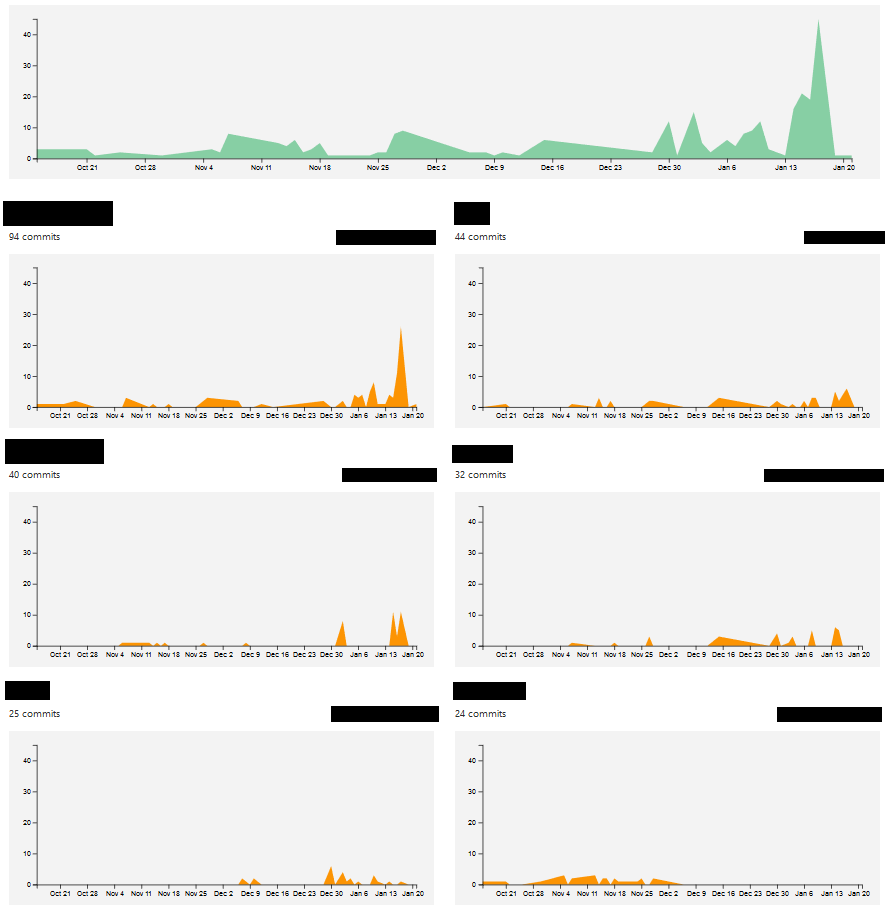
\includegraphics[scale=0.4]{slike/aktivnost.PNG}
			\centering
			\caption{Primjer slike s potpisom}
			\label{fig:promjene}
		\end{figure}
		
		\begin{figure}[H]
			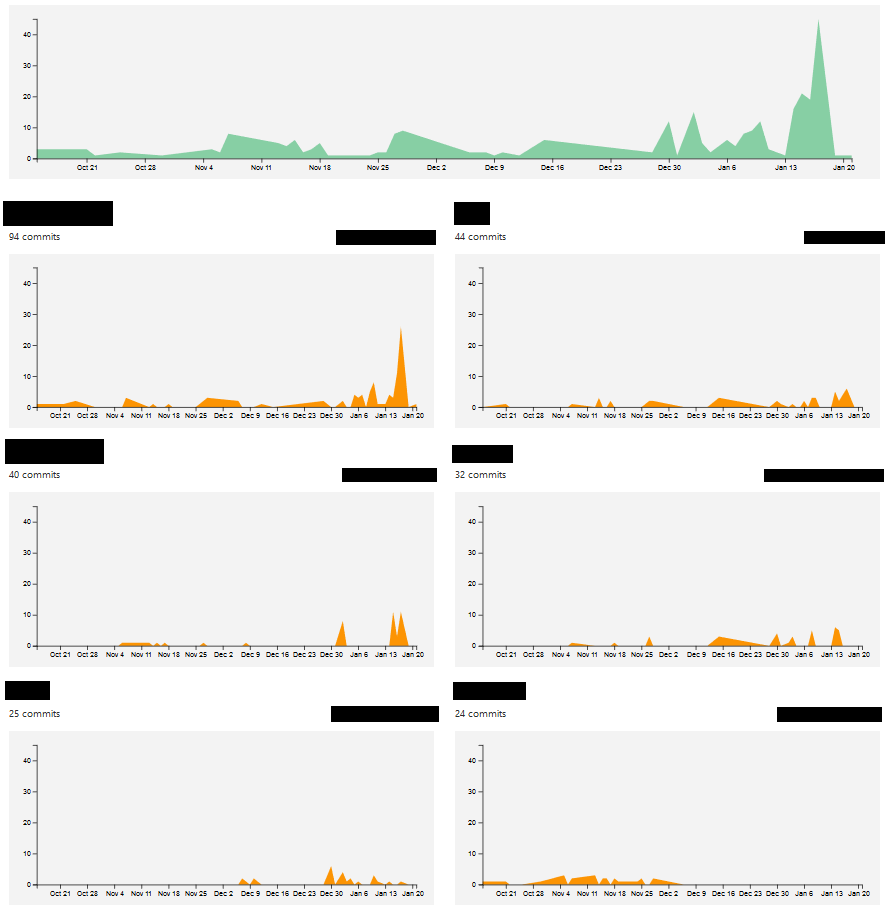
\includegraphics[width=\linewidth]{slike/aktivnost.PNG}
			\caption{Primjer slike s potpisom 2}
			\label{fig:promjene2}
		\end{figure}
		
		
		
		\eject
		
	
	\chapter{Specifikacija programske potpore}
		
	\section{Funkcionalni zahtjevi}
			
			\textbf{\textit{dio 1. revizije}}\\
			
			\textit{Navesti \textbf{dionike} koji imaju \textbf{interes u ovom sustavu} ili  \textbf{su nositelji odgovornosti}. To su prije svega korisnici, ali i administratori sustava, naručitelji, razvojni tim.}\\
				
			\textit{Navesti \textbf{aktore} koji izravno \textbf{koriste} ili \textbf{komuniciraju sa sustavom}. Oni mogu imati inicijatorsku ulogu, tj. započinju određene procese u sustavu ili samo sudioničku ulogu, tj. obavljaju određeni posao. Za svakog aktora navesti funkcionalne zahtjeve koji se na njega odnose.}\\
			
			
			\noindent \textbf{Dionici:}
			
			\begin{packed_enum}
				
				\item Dionik 1
				\item Dionik 2				
				\item ...
				
			\end{packed_enum}
			
			\noindent \textbf{Aktori i njihovi funkcionalni zahtjevi:}
			
			
			\begin{packed_enum}
				\item  \underbar{Aktor 1 (inicijator) može:}
				
				\begin{packed_enum}
					
					\item funkcionalnost 1
					\item funkcionalnost 2
					\begin{packed_enum}
						
						\item  podfunkcionalnost 1 
						\item  podfunkcionalnost 2
				
					\end{packed_enum}
					\item  funkcionalnost 3
					
				\end{packed_enum}
			
				\item  \underbar{Aktor 2 (sudionik) može:}
				
				\begin{packed_enum}
					
					\item funkcionalnost 1
					\item funkcionalnost 2
					
				\end{packed_enum}
			\end{packed_enum}
			
			\eject 
			
			
				
			\subsection{Obrasci uporabe}
				
				\textbf{\textit{dio 1. revizije}}
				
				\subsubsection{Opis obrazaca uporabe}
					\textit{Funkcionalne zahtjeve razraditi u obliku obrazaca uporabe. Svaki obrazac je potrebno razraditi prema donjem predlošku. Ukoliko u nekom koraku može doći do odstupanja, potrebno je to odstupanje opisati i po mogućnosti ponuditi rješenje kojim bi se tijek obrasca vratio na osnovni tijek.}\\
					

					\noindent \underbar{\textbf{UC$<$broj obrasca$>$ -$<$ime obrasca$>$}}
					\begin{packed_item}
	
						\item \textbf{Glavni sudionik: }$<$sudionik$>$
						\item  \textbf{Cilj:} $<$cilj$>$
						\item  \textbf{Sudionici:} $<$sudionici$>$
						\item  \textbf{Preduvjet:} $<$preduvjet$>$
						\item  \textbf{Opis osnovnog tijeka:}
						
						\item[] \begin{packed_enum}
	
							\item $<$opis korak jedan$>$
							\item $<$opis korak dva$>$
							\item $<$opis korak tri$>$
							\item $<$opis korak četiri$>$
							\item $<$opis korak pet$>$
						\end{packed_enum}
						
						\item  \textbf{Opis mogućih odstupanja:}
						
						\item[] \begin{packed_item}
	
							\item[2.a] $<$opis mogućeg scenarija odstupanja u koraku 2$>$
							\item[] \begin{packed_enum}
								
								\item $<$opis rješenja mogućeg scenarija korak 1$>$
								\item $<$opis rješenja mogućeg scenarija korak 2$>$
								
							\end{packed_enum}
							\item[2.b] $<$opis mogućeg scenarija odstupanja u koraku 2$>$
							\item[3.a] $<$opis mogućeg scenarija odstupanja  u koraku 3$>$
							
						\end{packed_item}
					\end{packed_item}

				\noindent \underbar{\textbf{UC2 - Pregled profila benda}}
				\begin{packed_item}
	
						\item \textbf{Glavni sudionik: }Javnost
						\item  \textbf{Cilj:} Pregledati profil benda
						\item  \textbf{Sudionici:} baza podataka,bend
						\item  \textbf{Preduvjet:} /
						\item  \textbf{Opis osnovnog tijeka:}
						
						\item[] \begin{packed_enum}
							\item Javnos odabire profil benda koji želi pregledati
							\item Aplikacija prikazuje profil be
							\item Aplikacija korisniku prikaže recenziju eventa
						\end{packed_enum}
				
				\end{packed_item}
				
				
				\noindent \underbar{\textbf{UC3 - Pregled recenzija}}
				\begin{packed_item}
	
						\item \textbf{Glavni sudionik: }Javnost
						\item  \textbf{Cilj:} Omogućiti pregled recenzija javnosti
						\item  \textbf{Sudionici:} baza podataka
						\item  \textbf{Preduvjet:} /
						\item  \textbf{Opis osnovnog tijeka:}
						
						\item[] \begin{packed_enum}
	
							\item Javna osoba pristupi popisu recenzija evenata
							\item Osoba odabere recenziju koju želi vidjeti
							\item Aplikacija korisniku prikaže recenziju eventa
						\end{packed_enum}
				\end{packed_item}

				
				\noindent \underbar{\textbf{UC4 - Registracija}}
				\begin{packed_item}
	
						\item \textbf{Glavni sudionik: }Korisnik
						\item  \textbf{Cilj:} Registrirati se
						\item  \textbf{Sudionici:} Baza podataka
						\item  \textbf{Preduvjet:} /
						\item  \textbf{Opis osnovnog tijeka:}
						
						\item[] \begin{packed_enum}
	
							\item Korisnik odabire opciju za registraciju
							\item Korisnik unosi potrebne korisničke podatke
							\item Korisnik prima obavijest o uspješnoj registraciji
						\end{packed_enum}
						
						\item[] \begin{packed_item}
	
							\item[1] Odabir već zauzetog korisničkog imena i/ili e-maila, unos podataka u        nedozvoljenom format ili pružanje neispravnog e-maila.
							\item[] \begin{packed_enum}
								
								\item  Sustav obavještava korisnika o neuspjelom upisu i vraća ga na stranicu za registraciju.
								\item Korisnik mijenja potrebne podatke ili odustaje od registracije.

							\end{packed_enum}
						\end{packed_item}						
				\end{packed_item}

				\newpage
				\noindent \underbar{\textbf{UC5 - Prijava u sustav}}
				\begin{packed_item}
	
						\item \textbf{Glavni sudionik: } Administrator, korisnik
						\item  \textbf{Cilj:} Korištenje sustava
						\item  \textbf{Sudionici:} baza podataka
						\item  \textbf{Preduvjet:} Autorizacija korisničkog imena i lozinke
						\item  \textbf{Opis osnovnog tijeka:}
						
						\item[] \begin{packed_enum}
	
							\item Korisnik unosi korisničko ime i lozinku
							\item Baza autorizira unesene podatke
							\item[] \begin{packed_enum}
								
								\item Dozvoljava korisniku korištenje sustava ako su podaci ispravni
								\item   Ne dozvoljava korisniku korištenje sustava ako su podaci ne ispravni
								
							\end{packed_enum}
						\end{packed_enum}
				\end{packed_item}


				\noindent \underbar{\textbf{UC6 - Uvid u popis dodanih instrumenata}}
				\begin{packed_item}
	
						\item \textbf{Glavni sudionik: }Administrator
						\item  \textbf{Cilj:} Pregled dodanih instrumenata od strane glazbenika.Uklanjanje nepotrebnih zapisa u bazi podataka (npr. "Gitara", "gitara")
						\item  \textbf{Sudionici:} baza podataka
						\item  \textbf{Preduvjet:} Glazbenici su dodali svoje instrumente i ti instrumenti su zapisani u bazi podataka
						\item  \textbf{Opis osnovnog tijeka:}
						
						\item[] \begin{packed_enum}
	
							\item Administrator odabire pregled dodanih instrumenata
							\item Ispis dodanih instrumenata
						\end{packed_enum}
				\end{packed_item}


				\noindent \underbar{\textbf{UC9 - Slanje poruka}}
				\begin{packed_item}

					\item \textbf{Glavni sudionik: }Administrator, glazbenik, korisnik
					\item  \textbf{Cilj:} Komunnikacija između korisnika
					\item  \textbf{Sudionici:} Baza podataka
					\item  \textbf{Preduvjet:} Korisnik je prijavljen
					\item  \textbf{Opis osnovnog tijeka:}
					
					\item[] \begin{packed_enum}

							\item Korisnik odabire "poruke"
							\item Aplikacija prikazuje pregled osoba s kojima se već vodio razgovor
							\item Korisnik odabire postojeći razgovor i prikazuju mu se prošle poruke
							\item Korisnik odabire "nova poruka" te pronalazi korisnika kojemu želi poslati poruku
							\item Korisnik odabire polje za pisanje poruke
							\item Korisnik napiše željenu poruku
							\item Korisnik odabere "Pošalji" za slanje poruke
					\end{packed_enum}
				
					\item  \textbf{Opis mogućih odstupanja:}
				
					\item[] \begin{packed_item}

						\item[2.a] Korisnik ima novih poruka
						\item[] \begin{packed_enum}
							\item Ukoliko postoji nova poruka, ime pošiljatelja je podebljano
						\end{packed_enum}
					\end{packed_item}
				\end{packed_item}
			
			\noindent \underbar{\textbf{UC10 - Pisanje recenzija o bendovima}}
			\begin{packed_item}
				
				\item \textbf{Glavni sudionik: }Korisnik
				\item  \textbf{Cilj:} Omogućiti korisnicima aplikacije pisanje recenzija o bendovima
				\item  \textbf{Sudionici:} Baza podataka, bend
				\item  \textbf{Preduvjet:} Korisnik mora biti prijavljen
				\item  \textbf{Opis osnovnog tijeka:} 
				
				\item[] \begin{packed_enum}
					
					\item Korisnik pristupa profilu benda
					\item U okvir za poruku napiše svoje mišljenje o bendu te označi broj zvjezdica kao ocjenu
					\item Korisnik odabere "Završi recenziju"
				\end{packed_enum}
			\end{packed_item}
				
			\noindent \underbar{\textbf{UC11 - Pisanje recenzija za događaje}}
			\begin{packed_item}
				
				\item \textbf{Glavni sudionik: }Korisnik
				\item  \textbf{Cilj:} Napisati recenziju za događaj
				\item  \textbf{Sudionici:} Baza podataka
				\item  \textbf{Preduvjet:} Korisnik je prijavljen
				\item  \textbf{Opis osnovnog tijeka:} 
				
				\item[] \begin{packed_enum}
					
					\item Korisnik odabire opciju za recenziranje događaja
					\item Otvara se prozor za unos recenzije
					\item Korisnik unosi recenziju i potvrđuje se
					\item Recenzija se bilježi na stranici događaja
				\end{packed_enum}
			\end{packed_item}
		 
		    \noindent \underbar{\textbf{UC12 - Pregled profila glazbenika}}
		    \begin{packed_item}
		    	
		    	\item \textbf{Glavni sudionik: }Korisnik, glazbenik
		    	\item  \textbf{Cilj:} Pregled profilne stranice glazbenika 
		    	\item  \textbf{Sudionici:} Baza podataka
		    	\item  \textbf{Preduvjet:} Autorizacija korisničkog imena i lozinke
		    	\item  \textbf{Opis osnovnog tijeka:} 
		    	
		    	\item[] \begin{packed_enum}
		    		
		    		\item Korisnik odabire prikaz profila glazbenika
		    		\item Prikazuju mu se javni podaci glazbenika (kalendar, instrumenti, popis nastupa na kojima svira)
		    	\end{packed_enum}
		    \end{packed_item}
		 
		
		
				
				\subsubsection{Dijagrami obrazaca uporabe}
				
				
				
					
					\textit{Prikazati odnos aktora i obrazaca uporabe odgovarajućim UML dijagramom. Nije nužno nacrtati sve na jednom dijagramu. Modelirati po razinama apstrakcije i skupovima srodnih funkcionalnosti.}
				\eject				
				
				
			\subsection{Sekvencijski dijagrami}
				
				\textbf{\textit{dio 1. revizije}}\\
				
				\textit{Nacrtati sekvencijske dijagrame koji modeliraju najvažnije dijelove sustava (max. 4 dijagrama). Ukoliko postoji nedoumica oko odabira, razjasniti s asistentom. Uz svaki dijagram napisati detaljni opis dijagrama.}
				\eject
	
		\section{Ostali zahtjevi}
		
			\textbf{\textit{dio 1. revizije}}\\
		 
			 \textit{Nefunkcionalni zahtjevi i zahtjevi domene primjene dopunjuju funkcionalne zahtjeve. Oni opisuju \textbf{kako se sustav treba ponašati} i koja \textbf{ograničenja} treba poštivati (performanse, korisničko iskustvo, pouzdanost, standardi kvalitete, sigurnost...). Primjeri takvih zahtjeva u Vašem projektu mogu biti: podržani jezici korisničkog sučelja, vrijeme odziva, najveći mogući podržani broj korisnika, podržane web/mobilne platforme, razina zaštite (protokoli komunikacije, kriptiranje...)... Svaki takav zahtjev potrebno je navesti u jednoj ili dvije rečenice.}
			 
			 
			 
	
	\chapter{Arhitektura i dizajn sustava}
		
	Da bi dugoročno uštedjeli vrijeme, uložili smo dio vremena na konfiguriranje CI (engl. continuous integration) i CD (engl. continuous delivery) procesa. Za isporuku aplikacije odabrali smo Heroku.
	
	Heroku je jedna od najpoznatijih platformi za isporučivanje aplikacija koja se ističe svojom jednostavnošću. Za razliku od AWS-ovih servisa, koje smo također razmatrali, Heroku se sam brine oko instanci i arhitekture sustava na kojem se izvodi naša aplikacija. Zbog ograničenih resursa odlučili smo isporučiti aplikaciju na besplatnu instancu Heroku-a.
	
	Besplatna instanca Heroku-a ima određena ograničenja, a najupečatljivije od njih je način na koji se pokreće projekt.
	Heroku sam prepoznaje kojeg je tipa projekt pa da pokrenemo frontend i backend trebamo dvije instance.
	CD je integriran putem GitLab-ovih pipelinesa za koje je bilo potrebno napisati .gitlab-ci.yml datoteku u kojoj smo konfigurirali GitLab-ov pipeline. GitLab-ov pipeline konfiguriran je tako da se na svaki commit u dev grani izgradi aplikacija, pokrenu i uspješno završe testovi te krene isporuka aplikacije na Heroku.
	
	Da bi osigurali maksimalno vrijeme dostupnosti naše platforme, .yml datoteka također je konfigurirana tako da prilikom commita u master isporuči aplikaciju na druge dvije instance.
	Ukupno imamo četiri pokrenute instance Heroku-a, od koje su dvije backend, a dvije frontend. Backend i frontend imaju svaki svoju razvojnu i produkcijsku instancu. Poveznice na instance:
	\begin{itemize}
		\item \url{http://giger-fer.herokuapp.com/}
		\item \url{https://giger-fer-dev.herokuapp.com/}
		\item \url{https://giger-backend-dev.herokuapp.com/}
		\item \url{http://giger-backend.herokuapp.com/}
	\end{itemize}
	
	
	U skladu s time, Spring Boot aplikacija ima dvije .properties datoteke. Jedna od njih je namijenjena lokalnom izvođenju aplikacije te sadrži postavke lokalne PostgreSQL baze, dok je druga konfigurirana tako da postavke čita iz varijabli okruženja. Varijable okruženja postavljene su na Heroku tako da čak niti pristupom u git repozitorij vanjski korisnik ne može doći do akreditacije (credentials) kojima bi mogao pristupiti bazi.
	
	Prednost ostvarena automatiziranjem procesa isporuke jest povećanje vjerojatnosti uspješnosti iste te povećanje udjela dostupnosti aplikacije zbog dva para instanci servera.
	
	Uvidjevši prednosti korištenja CD-a, primijenili smo to znanje i na prevođenje dokumentacije. 
	Unutar repozitorija, osim pipeline-a za isporuku aplikacije, postoji pipeline za automatsko prevođenje dokumentacije čiji je rezultat .pdf dokument.\\
	Potencijalni prostor za napredak bio bi korištenje Docker tehnologije tako da prilikom pokretanja aplikacije korisnik ne mora imati instaliranu PostgreSQL bazu već ju pokrene u Docker kontejneru.
	
	Od mogućih arhitektura sustava, za svoj projekt smo odabrali objektno usmjerenu arhitekturu. Tu arhitekturu smo odabrali zato što se koristi u industriji te je de facto standard razvoja složenih programskih rješenja. Osim toga, ona je fleksibilna, omogućuje recikliranje koda te logički razdjeljuje sustav na više cjelina, što je bitno s obzirom da više ljudi radi na implementaciji aplikacije. Zahvaljujući modularnosti programskog rješenja, greške su lako ispravljive, a nove mogućnosti dodaju se bez poteškoća.

	Odlučili smo se za web aplikaciju, koja je prilagođena mobilnim uređajima, obzirom da glazbenici, a time i bendovi nemaju uvijek pristup računalu, a ne želimo da je korisnik ograničen samo na mobilne uređaje.\\

	Arhitekturu sustava možemo podijeliti na četiri podsustava:
		\begin{itemize}
			\item Web preglednik
			\item Web poslužitelj
    			\item Web aplikacija
			\item Baza podataka
		\end{itemize}

	
	
	Korisnik (javnost, glazbenik, bend, administrator) pristupa web aplikaciji uz pomoć svog web preglednika, s time da se u sredini nalazi web poslužitelj. Na njemu se nalazi aplikacija koju on pokreće, te uz pomoć protokola komunicira s korisnicima.

	Klijentski (frontend) dio aplikacije omogućuje da korisnik korištenjem sučelja može pristupiti serveru (backend) aplikacije. Ovisno o tome što korisnik hoće, taj server ima mogućnost spajanja na bazu podataka kako bi korisniku prikazao informacije.

	Backend je napisan u Javi 11, a kao razvojni okvir koristimo Java Spring Boot 2.2.0. Dodani su projekti Spring Data JPA kako bi backend mogao lako komunicirati s bazom, Spring Web MVC za rukovanje zahtjevima te Spring Security kako bi zaštitili aplikaciju od vanjskih napada. Za pregledniji kod koristimo Lombok.

	\begin{figure}[H]
		\begin{center}
			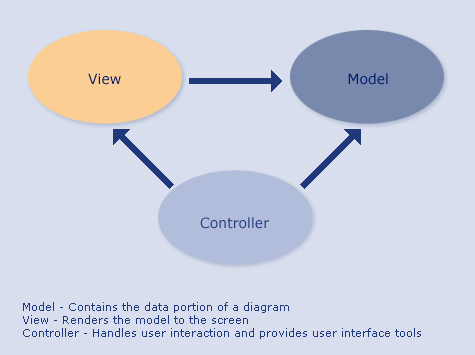
\includegraphics[width=10cm]{slike/mvc.PNG}
		\end{center}
		\caption{Pojednostavljeni prikaz MVC-a}
		\label{fig:mvc}
	\end{figure}

	Za frontend koristimo React. On je moderan i jednostavan framework koji koristi HTML, CSS, JSX i JavaScript uz pomoć kojeg smo napravili sučelje za našu aplikaciju. Uz pomoć React-a možemo lagano komunicirati s backendom koristeći REST.\\




		\section{Baza podataka}
		Za potrebe razvoja \textit{Gigera} koristit će se objektno relacijsko mapiranje. To je metoda koja se koristi u objektno-orijentiranim jezicima te se na taj način stvara virtualna objektna baza podataka. Za implementaciju baze podataka odabrali smo PostgreSQL, zbog generalno pozitivnog iskustva u korištenju te implementacije baze podataka u dosadašnjem fakultetskom obrazovanju. Bitno je naglasiti da na osobnim računalima u svrhu razvijanja aplikacije koristimo istu implementaciju baze kao i na web poslužitelju kako bi minimizirali neočekivano ponašanje.
		
		Baza podataka sastoji se od sljedećih tablica:
		
		\begin{packed_item}
		\item Comment
		\item Message
		\item Conversation
		\item Conversation\_user
		\item System\_person
		\item Person
		\item System\_person\_roles
		\item Organizer
		\item Band
		\item Gig\_type
		\item Band\_occasions
		\item Occasion
		\item Musician\_occasions
		\item Band\_invited\_back\_up\_members
		\item Band\_invited
		\item Band\_back\_up\_members
		\item Musician\_bands
		\item Post
		\item Musician
		\item Instruments
		\item Instrument
		\item Musician\_gig\_history
		\item Gig
		\item Review\_gig
		\item Review
		
	\end{packed_item}
	
	
	\subsection{Opis tablica}
	
	\textbf{Comment}
	Ovaj entitet sadrži jedan komentar. Sadrži atribute: id komentara, id autora, sadržaj te vrijeme objavljivanja. Ovaj entitet je u \textit{Many-to-One} vezi s entitetima: Post i Person.
	\begin{longtabu} to \textwidth {|X[6, l+3]|X[6, l]|X[20, l]|}
		

		\hline \multicolumn{3}{|c|}{\textbf{Comment}}	 \\[3pt] \hline
		\endfirsthead
		
		\hline 
		\endlastfoot
		
		\textbf{id} & BIGINT	&  	jedinstveni identifikator komentara 	\\ \hline
		content & VARCHAR & sadržaj komentara \\ \hline
		posted\_on & TIMESTAMP & datum i vrijeme objave komentara \\ \hline	
		\textit{author\_id} & BIGINT & jedinstveni identifikator autora komentara \\ \hline
		\textit{fk\_post} & BIGINT & jedinstveni identifikator komentara \\ \hline
		
	\end{longtabu}
	
	\textbf{Message}
	Ovaj entitet sadrži informacije o poruci. Sadrži atribute: id poruke, sadržaj poruke, vrijeme kada je poruka poslana, id pošiljatelja i id razgovora. Ovaj entitet je u \textit{Many-to-One} vezi s entitetima: Conversation, Person, Band. Ako je bend poslao poruku, tada je fk\_sender null, a ako ju je poslao korisnik tada je fk\_sender\_band null.
	\begin{longtabu} to \textwidth {|X[6, l+3]|X[6, l]|X[20, l]|}
		
		\hline \multicolumn{3}{|c|}{\textbf{Message}}	 \\[3pt] \hline
		\endfirsthead
		
		\hline
		\endlastfoot
		
		\textbf{id} & BIGINT	&  	jedinstveni identifikator poruke 	\\ \hline
		content	& VARCHAR & sadržaj poruke	\\ \hline
		sent\_time & TIMESTAMP & vrijeme kada je poruka poslana \\ \hline
		\textit{fk\_sender} & BIGINT & jedinstveni identifikator pošiljatelja \\ \hline
		\textit{fk\_sender\_band} & BIGINT & jedinstveni identifikator benda pošiljatelja \\ \hline
		\textit{fk\_converation} & BIGINT & jedinstveni identifikator razgovora \\ \hline
		
	\end{longtabu}
	
	\textbf{Conversation}
	Ovaj entitet sadrži informacije o razgovoru. Sadrži atribute: id razgovora i ime razgovora. Ovaj entitet je u \textit{One-to-Many} vezi s entitetima: Message i
	\emph{Many-to-One} vezi s entitetima: Band i Person.
	\begin{longtabu} to \textwidth {|X[6, l+3]|X[6, l]|X[20, l]|}
		
		\hline \multicolumn{3}{|c|}{\textbf{Conversation}}	 \\[3pt] \hline
		\endfirsthead
		
		\hline
		\endlastfoot
		
		\textbf{id} & BIGINT	&  	jedinstveni identifikator razgovora 	\\ \hline
		\textit{fk\_band} & BIGINT & jedinstveni identifikator benda \\ \hline
		picture\_url & VARCHAR & url slike razgovora \\ \hline
		title	& VARCHAR &  naziv razgovora	\\ \hline
		
	\end{longtabu}
	
	\textbf{Conversation\_user}
	Ova vezna tablica sadrži informacije o sudjelovanju korisniku u razgovoru. Sadrži atribute: id korisnika i id razgovora.
	\begin{longtabu} to \textwidth {|X[6, l+3]|X[6, l]|X[20, l]|}
		
		\hline \multicolumn{3}{|c|}{\textbf{Conversation\_user}}	 \\[3pt] \hline
		\endfirsthead
		
		\hline
		\endlastfoot
		
		\textbf{fk\_user} & BIGINT	&  	jedinstveni identifikator korisnika	\\ \hline
		\textbf{fk\_conversation}	& BIGINT &  jedinstveni identifikator razgovora	\\ \hline
		
	\end{longtabu}
	
	\textbf {System\_Person}
	Ovaj entitet sadrži podatke korisnika potrebne sustavu za sistemsku logiku.  Sadrži atribute: id korisnika, email, locked i verified zastavice te šifriranu lozinku. Ovaj entitet je u \emph{One-to-Many} vezi s entitetom: Roles i \emph{One-to-One} vezi s entitetima: Person, Musician i Organizer.
	\begin{longtabu} to \textwidth {|X[6, l+3]|X[6, l]|X[20, l]|}
		
		\hline \multicolumn{3}{|c|}{\textbf{System\_person}}	 \\[3pt] \hline
		\endfirsthead
		
		\hline
		\endlastfoot
		
		\textbf{id} & BIGINT	&  	jedinstveni identifikator sustavskih podataka o korisniku	\\ \hline
		email & VARCHAR & email adresa osobe \\ \hline
		locked & BOOLEAN & korisnik ima zabranu korištenja aplikacije ili ne \\ \hline
		password\_hash & VARCHAR & hash lozinke osobe \\ \hline
		verified & BOOLEAN & email adresa potvrđena ili ne \\ \hline
		
	\end{longtabu}
	
		\textbf{Person}
	Ovaj entitet sadrži podatke korisnika potrebne za poslovne svrhe.  Sadrži atribute: telefonski broj, url slike korisnika, korisničko ime kojim se predstavlja javnosti. Ovaj entitet je u \emph{One-to-Many} vezi s entitetima: Conversation, Message i
	\emph{One-to-One} vezi s entitetima: Musician, System\_person i Organizer.
	\begin{longtabu} to \textwidth {|X[6, l+3]|X[6, l]|X[20, l]|}
		
		\hline \multicolumn{3}{|c|}{\textbf{Person}}	 \\[3pt] \hline
		\endfirsthead
		
		\hline
		\endlastfoot
		
		\textbf{id} & BIGINT	&  	jedinstveni identifikator korisnika	\\ \hline
		phone\_number & VARCHAR & telefonski broj korisnika \\ \hline
		picture\_url & VARCHAR & url slike korisnika \\ \hline
		username & VARCHAR & korisničko ime korisnika
		
	\end{longtabu}
	
		\textbf{System\_person\_roles}
	Ovo je vezna tablica koja sadrži n-torke iz kojih možemo iščitati dodijeljene uloge pojedinim korisnicima. Sadrži atribute: system\_person\_id i cijeli broj uloge koji predstavlja enumeraciju.
	\begin{longtabu} to \textwidth {|X[6, l+3]|X[6, l]|X[20, l]|}
		
		\hline \multicolumn{3}{|c|}{\textbf{System\_person\_roles}}	 \\[3pt] \hline
		\endfirsthead
		
		\hline
		\endlastfoot
		
		\textbf{system\_person\_id} & BIGINT	&  	jedinstveni identifikator sustavskih podataka o korisniku	\\ \hline
		\textbf{roles} & INT & uloga korisnika \\ \hline
		
		
	\end{longtabu}
	
	\textbf {Organizer}
	Ovaj entitet sadrži informacije o organizatoru. Sadrži atribute: id organizatora te ime organizatora. Ovaj entitet je u \emph{One-to-One} vezi s entitetima: Musician, System\_person i Organizer te u \emph{One-to-Many} vezi s entitetom Gig.
	\begin{longtabu} to \textwidth {|X[6, l+3]|X[6, l]|X[20, l]|}
		
		\hline \multicolumn{3}{|c|}{\textbf{Organizer}}	 \\[3pt] \hline
		\endfirsthead
		
		\hline
		\endlastfoot
		
		\textbf{id} & BIGINT	&  	jedinstveni identifikator organizatora 	\\ \hline
		manager\_name	& VARCHAR &  ime organizatora	\\ \hline
		
	\end{longtabu}

\textbf{Band}
Ovaj entitet sadrži podatke o kreiranom bendu.  Sadrži atribute: id, opis, datum formiranja, adresu sjedišta, dodatni opis adrese, par koordinata, maksimalnu udaljenost, naziv benda, url slike benda i id voditelja benda. Ovaj entitet je u \textit{Many-to-Many} vezi s Musician za potrebe liste članova, u \textit{Many-to-One} vezi s Musician za potrebu evidencije voditelja benda te \emph{One-to-Many} vezi s entitetima: Message, Conversation, Gig i Post.

	\begin{longtabu} to \textwidth {|X[6, l+3]|X[6, l]|X[20, l]|}
		
		\hline \multicolumn{3}{|c|}{\textbf{Band}}	 \\[3pt] \hline
		\endfirsthead
		
		\hline 
		\endlastfoot
		
		\textbf{id} & BIGINT	&  	jedinstveni identifikator benda 	\\ \hline
		bio & VARCHAR & opis benda \\ \hline
		formed\_date & DATE & datum osnutka benda \\ \hline
		address & VARCHAR & adresa benda \\ \hline
		extra\_description & VARCHAR & dodatak opis benda \\ \hline
		x & DOUBLE & x koordinata lokacije \\ \hline
		y & DOUBLE & y koordinata lokacije \\ \hline
		max\_distance & DOUBLE & najveća udaljenost koju bend želi prijeći zbog gaže \\ \hline
		name & VARCHAR & ime benda \\ \hline
		picture\_url & VARCHAR & url slike benda \\ \hline
		\textit{leader\_id}	& BIGINT &  jedinstveni identifikator voditelja benda	\\ \hline 	
		
	\end{longtabu}
	
			\textbf {Gig\_type}
	Ovo je vezna tablica iz koje se mogu iščitati sve vrste nastupa koje izvodi određeni bend. Sadrži atribute: band\_id i naziv tipa nastupa.
	\begin{longtabu} to \textwidth {|X[6, l+3]|X[6, l]|X[20, l]|}

		\hline \multicolumn{3}{|c|}{\textbf{Gig\_type}}	 \\[3pt] \hline
		\endfirsthead

		\hline
		\endlastfoot

		\textbf{band\_id} &  BIGINT	&  	jedinstveni identifikator benda 	\\ \hline
		\textbf{gig\_type}	& VARCHAR &  vrsta nastupa	\\ \hline

	\end{longtabu}

				\textbf {Band\_occasions}
	Ovo je vezna tablica iz koje se može iščitati zauzetost benda. Sadrži atribute: identifikator benda i identifikator termina.
	\begin{longtabu} to \textwidth {|X[6, l+3]|X[6, l]|X[20, l]|}

		\hline \multicolumn{3}{|c|}{\textbf{Band\_occasions}}	 \\[3pt] \hline
		\endfirsthead

		\hline
		\endlastfoot

		\textbf{occasion\_id} &  BIGINT	&  	jedinstveni identifikator događaja 	\\ \hline
		\textbf{band\_id} &  BIGINT	&  	jedinstveni identifikator benda koji sudjeluje na događaju 	\\ \hline

	\end{longtabu}


		\textbf{Occasion}
	Ovaj entitet sadrži podatke o događaju. Sadrži atribute: id događaja, opis, datum, zastavicu privatnosti. Ovaj entitet je u \textit{Many-to-One} vezi s entitetima: Musician i Band.
	\begin{longtabu} to \textwidth {|X[6, l+3]|X[6, l]|X[20, l]|}
		
		\hline \multicolumn{3}{|c|}{\textbf{Occasion}}	 \\[3pt] \hline
		\endfirsthead
		
		\hline 
		\endlastfoot
		
		\textbf{id} &  BIGINT	&  	jedinstveni identifikator događaja 	\\ \hline
		description & VARCHAR & opis događaja \\ \hline
		local\_date & DATE & datum održavanja događaja \\ \hline
		personal\_occasion & BOOLEAN & privatan događaj ili ne \\ \hline

		
		
	\end{longtabu}
	
		\textbf{Musician\_occasions}
	Ovo je vezna tablica iz koje se može iščitati zauzetost glazbenika. Sadrži atribute: identifikator glazbenika i identifikator termina.
	\begin{longtabu} to \textwidth {|X[6, l+3]|X[6, l]|X[20, l]|}
		
		\hline \multicolumn{3}{|c|}{\textbf{Musician\_occasions}}	 \\[3pt] \hline
		\endfirsthead
		
		\hline 
		\endlastfoot
		
		\textbf{musician\_id} &  BIGINT	&  	jedinstveni identifikator glazbenika 	\\ \hline
		\textbf{occasions\_id} &  BIGINT	&  	jedinstveni identifikator termina	\\ \hline
		
		
	\end{longtabu}
	
		\textbf{Band\_invited\_back\_up\_members}
	Ovo je vezna tablica iz koje se mogu iščitati poslane i neodgovorene pozivnice za pričuvnog člana benda. Sadrži atribute: identifikator glazbenika i identifikator benda.
	\begin{longtabu} to \textwidth {|X[6, l+11]|X[6, l]|X[20, l]|}
		
		\hline \multicolumn{3}{|c|}{\textbf{Band\_invited\_back\_up\_members}}	 \\[3pt] \hline
		\endfirsthead
		
		\hline 
		\endlastfoot
		
		\textbf{band\_id} &  BIGINT	&  	jedinstveni identifikator benda 	\\ \hline
		\textbf{invited\_back\_up\_members\_id} &  BIGINT	&  	jedinstveni identifikator glazbenika pozvanih u bend kao pričuvni član	\\ \hline
		
		
	\end{longtabu}
	
		\textbf{Band\_invited}
	Ovo je vezna tablica iz koje se mogu iščitati poslane i neodgovorene pozivnice za člana benda. Sadrži atribute: identifikator glazbenika i identifikator benda.
	\begin{longtabu} to \textwidth {|X[6, l+3]|X[6, l]|X[20, l]|}
		
		\hline \multicolumn{3}{|c|}{\textbf{Band\_invited}}	 \\[3pt] \hline
		\endfirsthead
		
		\hline 
		\endlastfoot
		
		\textbf{band\_id} &  BIGINT	&  	jedinstveni identifikator benda 	\\ \hline
		\textbf{invited\_id} &  BIGINT	&  	jedinstveni identifikator glazbenika pozvanih u bend	\\ \hline
		
		
	\end{longtabu}
	
			\textbf {Band\_back\_up\_members}
	Ovo je vezna tablica iz koje se mogu iščitati pričuvni članovi bendova. Sadrži atribute: identifikator glazbenika i identifikator benda.
	\begin{longtabu} to \textwidth {|X[6, l+11]|X[6, l]|X[20, l]|}
		
		\hline \multicolumn{3}{|c|}{\textbf{Band\_back\_up\_members}}	 \\[3pt] \hline
		\endfirsthead
		
		\hline 
		\endlastfoot
		
		\textbf{band\_id} &  BIGINT	&  	jedinstveni identifikator benda 	\\ \hline
		\textbf{invited\_back\_up\_members\_id} &  BIGINT	&  	jedinstveni identifikator glazbenika koji su pričuvni članovi	\\ \hline
		
		
	\end{longtabu}
	
			\textbf {Musician\_bands}
	Ovo je vezna tablica iz koje se mogu iščitati članovi bendova. Sadrži atribute: identifikator glazbenika i identifikator benda.
	\begin{longtabu} to \textwidth {|X[6, l+3]|X[6, l]|X[20, l]|}
		
		\hline \multicolumn{3}{|c|}{\textbf{Musician\_bands}}	 \\[3pt] \hline
		\endfirsthead
		
		\hline 
		\endlastfoot
		
		\textbf{fk\_musician} & BIGINT	&  	jedinstveni identifikator glazbenika 	\\ \hline
		\textbf{fk\_band}	& BIGINT &  jedinstveni identifikator benda	\\ \hline
		
	\end{longtabu}
	
	\textbf{Post}
	Ovaj entitet sadrži podatke o objavi. Sadrži atribute: id objave, sadržaj, datum i vrijeme objave, identifikator korisnika ili benda (autora). Ovaj entitet je u \textit{One-to-Many} vezi s entitetima: Comment te u \emph{Many-to-one} s entitetima: Person, Band.
	\begin{longtabu} to \textwidth {|X[6, l+3]|X[6, l]|X[20, l]|}
		
		\hline \multicolumn{3}{|c|}{\textbf{Post}}	 \\[3pt] \hline
		\endfirsthead
		
		\hline 
		\endlastfoot
		
		\textbf{id} & BIGINT	&  	jedinstveni identifikator objave 	\\ \hline
		content & VARCHAR & sadržaj objave \\ \hline
		published\_on & TIMESTAMP & datum i vrijeme objave \\ \hline
		\textit{fk\_band} & BIGINT & jedinstveni identifikator benda \\ \hline
		\textit{fk\_user} & BIGINT & jedinstveni identifikator korisnika koji je napisao objavu \\ \hline
		
	\end{longtabu}
	
		\textbf {Musician}
	Ovaj entitet sadrži informacije o glazbeniku. Sadrži atribute: id glazbenika, oznaku za privatan kalendar te opis glazbenika. Ovaj entitet je u \emph{One-to-One} vezi s entitetima: System\_person, Organizer i Person, u \emph{Many-to-Many} vezi s entitetima: Instrument i Band te u \emph{One-to-Many} vezi s entitetima: Band (u potrebe pohranjivanja voditelja benda) i Occasions.
	\begin{longtabu} to \textwidth {|X[6, l+3]|X[6, l]|X[20, l]|}
		
		\hline \multicolumn{3}{|c|}{\textbf{Musician}}	 \\[3pt] \hline
		\endfirsthead
		
		\hline 
		\endlastfoot
		
		\textbf{id} & BIGINT	&  	jedinstveni identifikator glazbenika 	\\ \hline	
		bio	& VARCHAR &  opis glazbenika	\\ \hline 
		public\_calendar & BOOLEAN & kalendar glazbenika javan ili ne \\ \hline
			
		
	\end{longtabu}
	
	\textbf{Instruments}
	Ovo je vezna tablica iz koje se može iščitati koje instrumente svira pojedini glazbenik. Sadrži atribute: id instrumenta te id glazbenika.
	\begin{longtabu} to \textwidth {|X[6, l+3]|X[6, l]|X[20, l]|}
		
		\hline \multicolumn{3}{|c|}{\textbf{Instruments}}	 \\[3pt] \hline
		\endfirsthead
		
		\hline 
		\endlastfoot
		
		\textbf{instruments\_id} & BIGINT & jedinstveni identifikator instrumenta \\ \hline
		\textbf{musician} & BIGINT	&  	jedinstveni identifikator glazbenika	\\ \hline
		
		
	\end{longtabu}
	
	\textbf{Instrument}
	Ovaj entitet sadrži informacije o instrumentima. Sadrži atribute: id instrumenta, ime instrumenta te vrstu instrumenta. Ovaj entitet je u \emph{One-to-Many} vezi s entitetom Musician.
	\begin{longtabu} to \textwidth {|X[6, l+3]|X[6, l]|X[20, l]|}
		
		\hline \multicolumn{3}{|c|}{\textbf{Instrument}}	 \\[3pt] \hline
		\endfirsthead
		
		\hline 
		\endlastfoot
		
		\textbf{id} & BIGINT & jedinstveni identifikator instrumenta \\ \hline
		name & VARCHAR & ime instrumenta \\ \hline
		type & INT & vrsta instrumenta \\ \hline
		
		
	\end{longtabu}
	
		\textbf{Musician\_gig\_history}
	Ovo je vezna tablica iz koje se može iščitati povijest nastupa glazbenika. Sadrži atribute: identifikator glazbenika i identifikator nastupa.
	\begin{longtabu} to \textwidth {|X[6, l+3]|X[6, l]|X[20, l]|}
		
		\hline \multicolumn{3}{|c|}{\textbf{Musician\_gig\_history}}	 \\[3pt] \hline
		\endfirsthead
		
		\hline 
		\endlastfoot
		
		\textbf{fk\_musician} & BIGINT & jedinstveni identifikator glazbenika \\ \hline
		\textbf{fk\_gig} & BIGINT & jedinstveni identifikator nastupa \\ \hline
		
		
		
	\end{longtabu}
	
	\textbf {Gig}
	Ovaj entitet sadrži informacije o nastupima. Sadrži atribute: id nastupa, datum i vrijeme održavanja nastupa, opis nastupa, očekivano trajanje nastupa, oznaku za postignut dogovor, vrstu nastupa, adresa održavanja nastupa, dodatan opis nastupa, x koordinata lokacije, y koordinata lokacije, oznaku za privatan nastup, preporučenu cijenu ulaznice, id organizatora te id benda. Ovaj entitet je u \textit{Many-to-One} vezi s entitetima Organizer i Band te \textit{One-to-Many} vezi s entitetom Review i u \emph{Many-to-Many} vezi s entitetom Musician.
	\begin{longtabu} to \textwidth {|X[6, l+3]|X[6, l]|X[20, l]|}
		
		\hline \multicolumn{3}{|c|}{\textbf{Gig}}	 \\[3pt] \hline
		\endfirsthead
		
		\hline 
		\endlastfoot
		
		\textbf{id} & BIGINT	&  	jedinstveni identifikator nastupa 	\\ \hline
		date\_time & TIMESTAMP & datum i vrijeme održavanja nastupa \\ \hline
		description & VARCHAR & opis nastupa \\ \hline
		expected\_duration & VARCHAR & očekivano trajanje nastupa \\ \hline
		final\_deal\_achieved & BOOLEAN & dogovor postignut ili ne \\ \hline
		gig\_type & INT & vrsta nastupa \\ \hline
		address & VARCHAR & adresa održavanja nastupa \\ \hline
		extra\_description & VARCHAR & dodatan opis nastupa \\ \hline
		x & DOUBLE & x koordinata lokacije \\ \hline
		y & DOUBLE & y koordinata lokacije \\ \hline
		private\_gig & BOOLEAN & nastupa privatan ili ne \\ \hline
		proposed\_price & INT & preporučena cijena ulaznice \\ \hline
		\textit{organizer\_id}	& BIGINT &  jedinstveni identifikator organizatora	\\ \hline 	
		\textit{band\_id}	& BIGINT &  jedinstveni identifikator benda	\\ \hline 	
		
	\end{longtabu}
	
	\textbf {Review\_gig}
	Ovo je vezna tablica iz koje pronalazimo pripadnost recenzije pojedinom nastupu. Sadrži atribute: id nastupa i id recenzije.
	\begin{longtabu} to \textwidth {|X[6, l+3]|X[6, l]|X[20, l]|}
		
		\hline \multicolumn{3}{|c|}{\textbf{Review\_gig}}	 \\[3pt] \hline
		\endfirsthead
		
		\hline 
		\endlastfoot
		
		\textbf{fk\_gig} & BIGINT	&  	jedinstveni identifikator nastupa 	\\ \hline
		\textbf{fk\_review}	& BIGINT &  jedinstveni identifikator recenzije	\\ \hline 		
		
	\end{longtabu}
	
	\textbf{Review}
	Ovaj entitet sadrži informacije za recenziju. Sadrži atribute: id recenzije, sadržaj recenzije benda, sadržaj recenzije organizatora, vrijeme objave recenzije, ocjenu benda, ocjenu organizatora te id autora. Ovaj entitet je u \emph{Many-to-One} vezi s entitetima: Musician i Organizer.
	
	\begin{longtabu} to \textwidth {|X[6, l+14]|X[6, l+2]|X[20, l]|}
		
		\hline \multicolumn{3}{|c|}{\textbf{Review}}	 \\[3pt] \hline
		\endfirsthead
		
		\hline
		\endlastfoot
		
		\textbf{id} & BIGINT	&  	jedinstveni identifikator recenzije 	\\ \hline
		content\_of\_review\_for\_band	& VARCHAR &  sadržaj komentara benda	\\ \hline
		content\_of\_review\_for\_organizer	& VARCHAR &  sadržaj komentara organizatora	\\ \hline
		created & TIMESTAMP & vrijeme objave komentara \\ \hline
		grade\_band & INT & ocjena benda \\ \hline
		grade\_organizer & INT & ocjena organizatora  \\ \hline
		\textit{author\_id} & BIGINT	& jedinstveni identifikator korisnika koji je autor recenzije	\\ \hline
		
		
	\end{longtabu}
	

		
	

			
			\subsection{Dijagram baze podataka}
			
			\begin{figure}[H]
			\begin{center}
				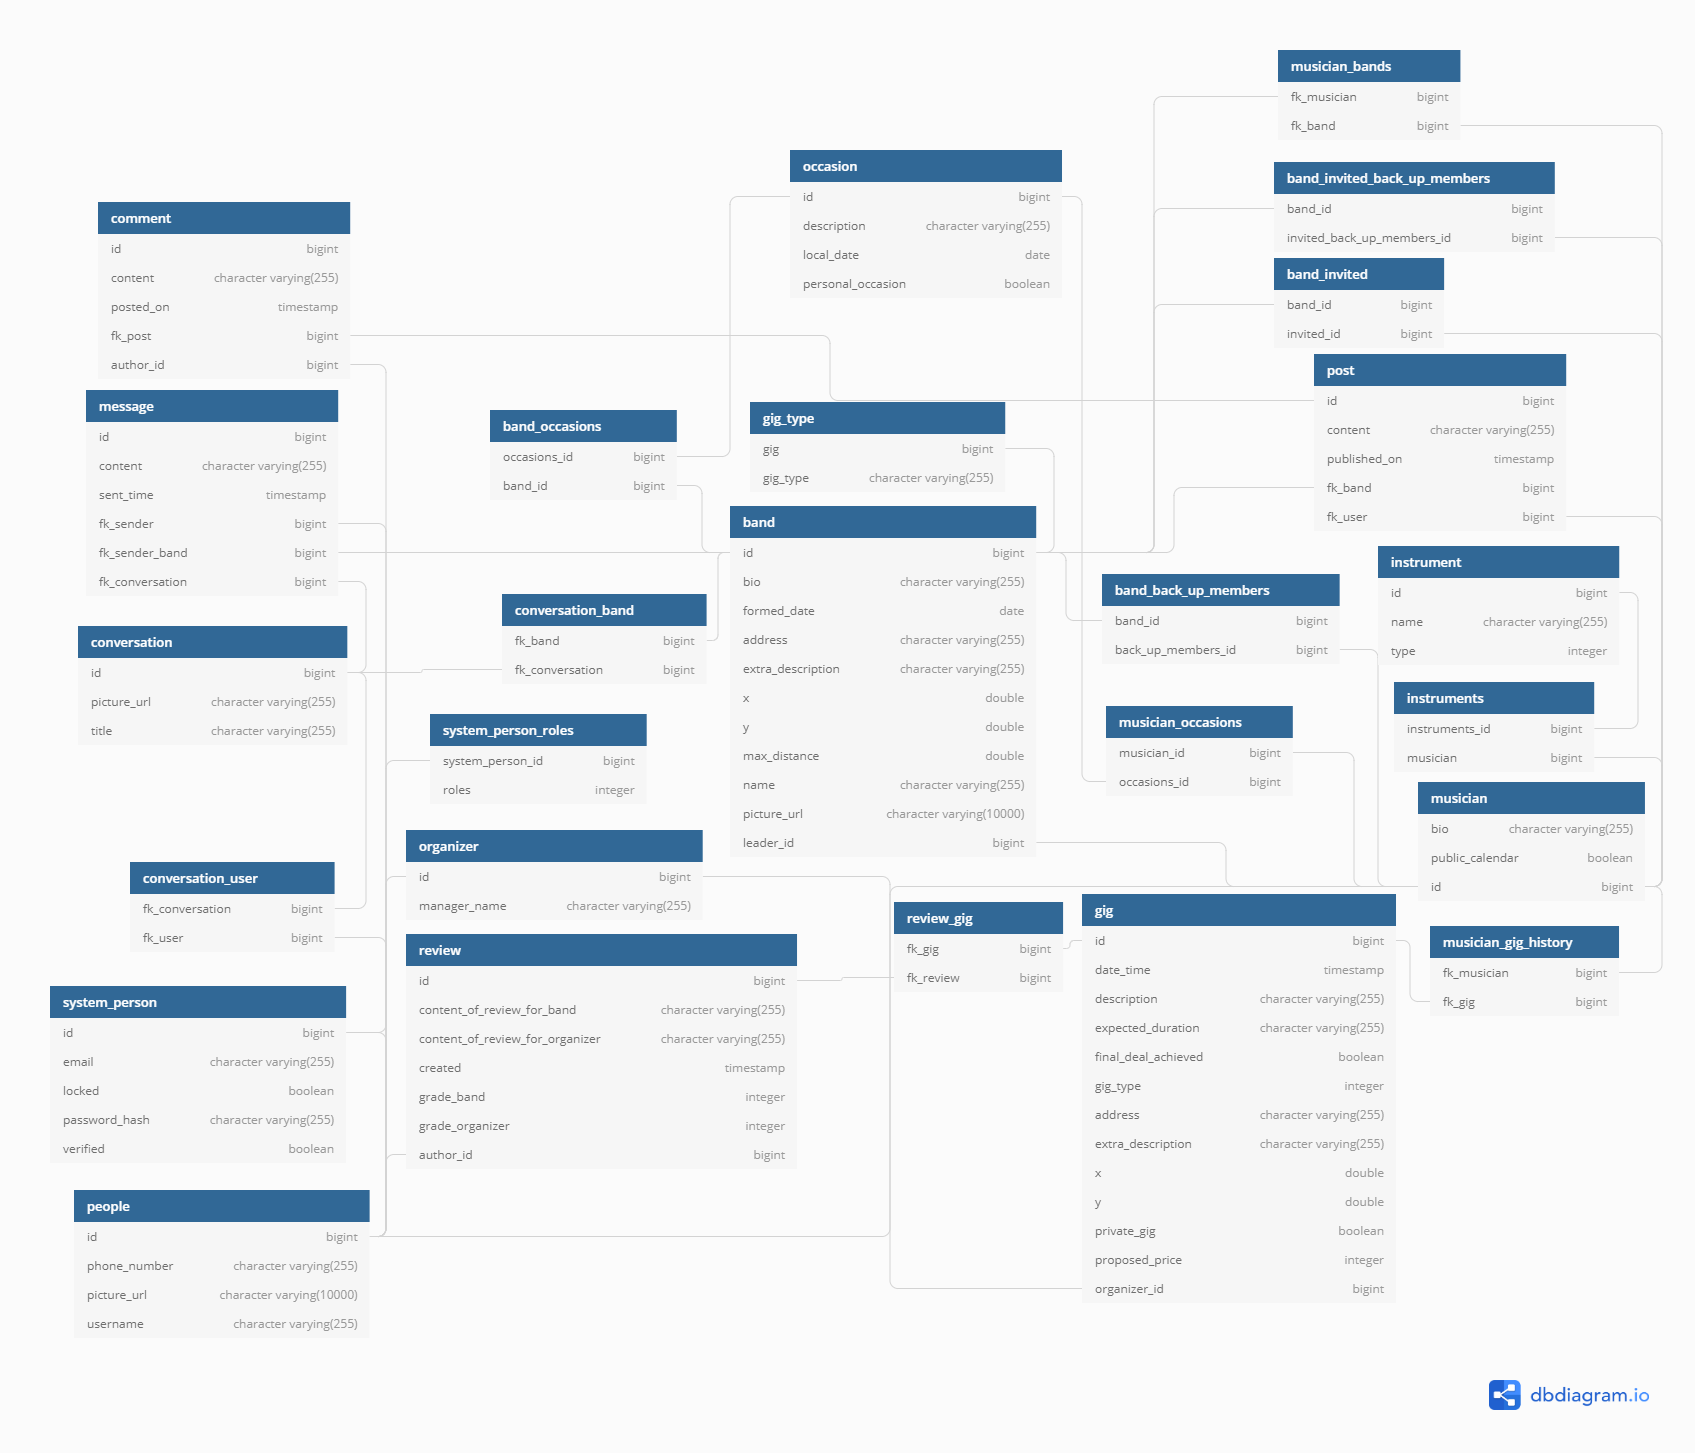
\includegraphics[width=17cm]{slike/ERModel.PNG}
			\end{center}
			\caption{Dijagram baze podataka}
			\label{fig:dijagramBaze}
		\end{figure}
			
			
			
		\section{Dijagram razreda}


			\textit{\textbf{dio 2. revizije}} \\
			
			\textit{Prilikom druge predaje projekta dijagram razreda i opisi moraju odgovarati stvarnom stanju implementacije} \\
			
			
			Na slici 4.3 prikazan je Controllers dio backend aplikacije. Controlleri su jedina izložena točka u aplikaciji te nad njima frontend izvršava upite. Svi Controller-i su zaštićeni Spring Security-jem te se prije svakog propuštanja zahtjeva na Controller autorizira token koji se nalazi u zaglavlju zahtjeva. Jedina iznimka su Controller-i koji služe za registraciju i prijavu. Nakon što se zahtjev autorizira Controller-i pozivaju servisni sloj aplikacije te od njih zahtjevaju da izvrše dio poslovne logike za koju su napisani. Povratni tip Controller-a su DTO-ovi (Data Transfer Objects) prikazani na slici 4.4. Njima se na frontend vraća samo dio informacije prikupljene od servisa.  

			\begin{figure}[H]
				\begin{center}
					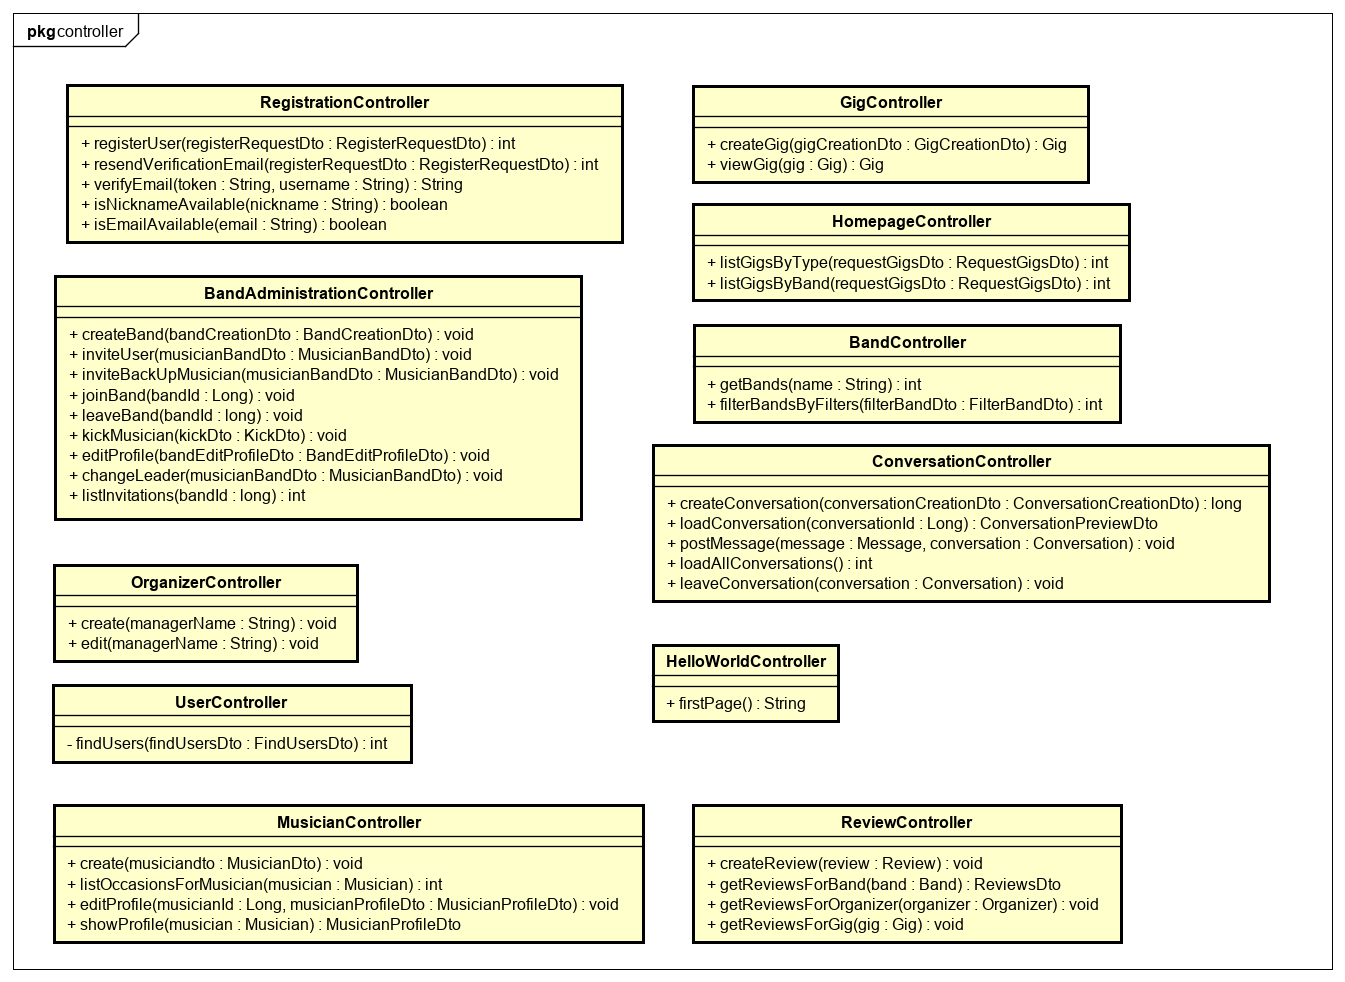
\includegraphics[width=17cm]{slike/kontroleri.PNG}
				\end{center}
				\caption{Dijagram razreda - dio Controllers}
				\label{fig:kontroleri}
			\end{figure}
		
			Slika 4.4 prikazuje DTO-ove kojima backend dio aplikacije komunicira s frontendom. DTO-ove smo modelirali tako da izbjegnemo kružne reference objekata koje dobijemo iz baze podataka. Kao posljedica, DTO-ovi sadrže uglavnom primitivne tipove ili neke druge DTO-ove (npr. ConversationPreviewDTO sadrži listu PersonPreviewDTO koji predstavljaju sudionike razgovora). DTO-ove koristimo u oba smjera komunikacije backenda i frontenda.
			
			
			\begin{figure}[H]
				\begin{center}
					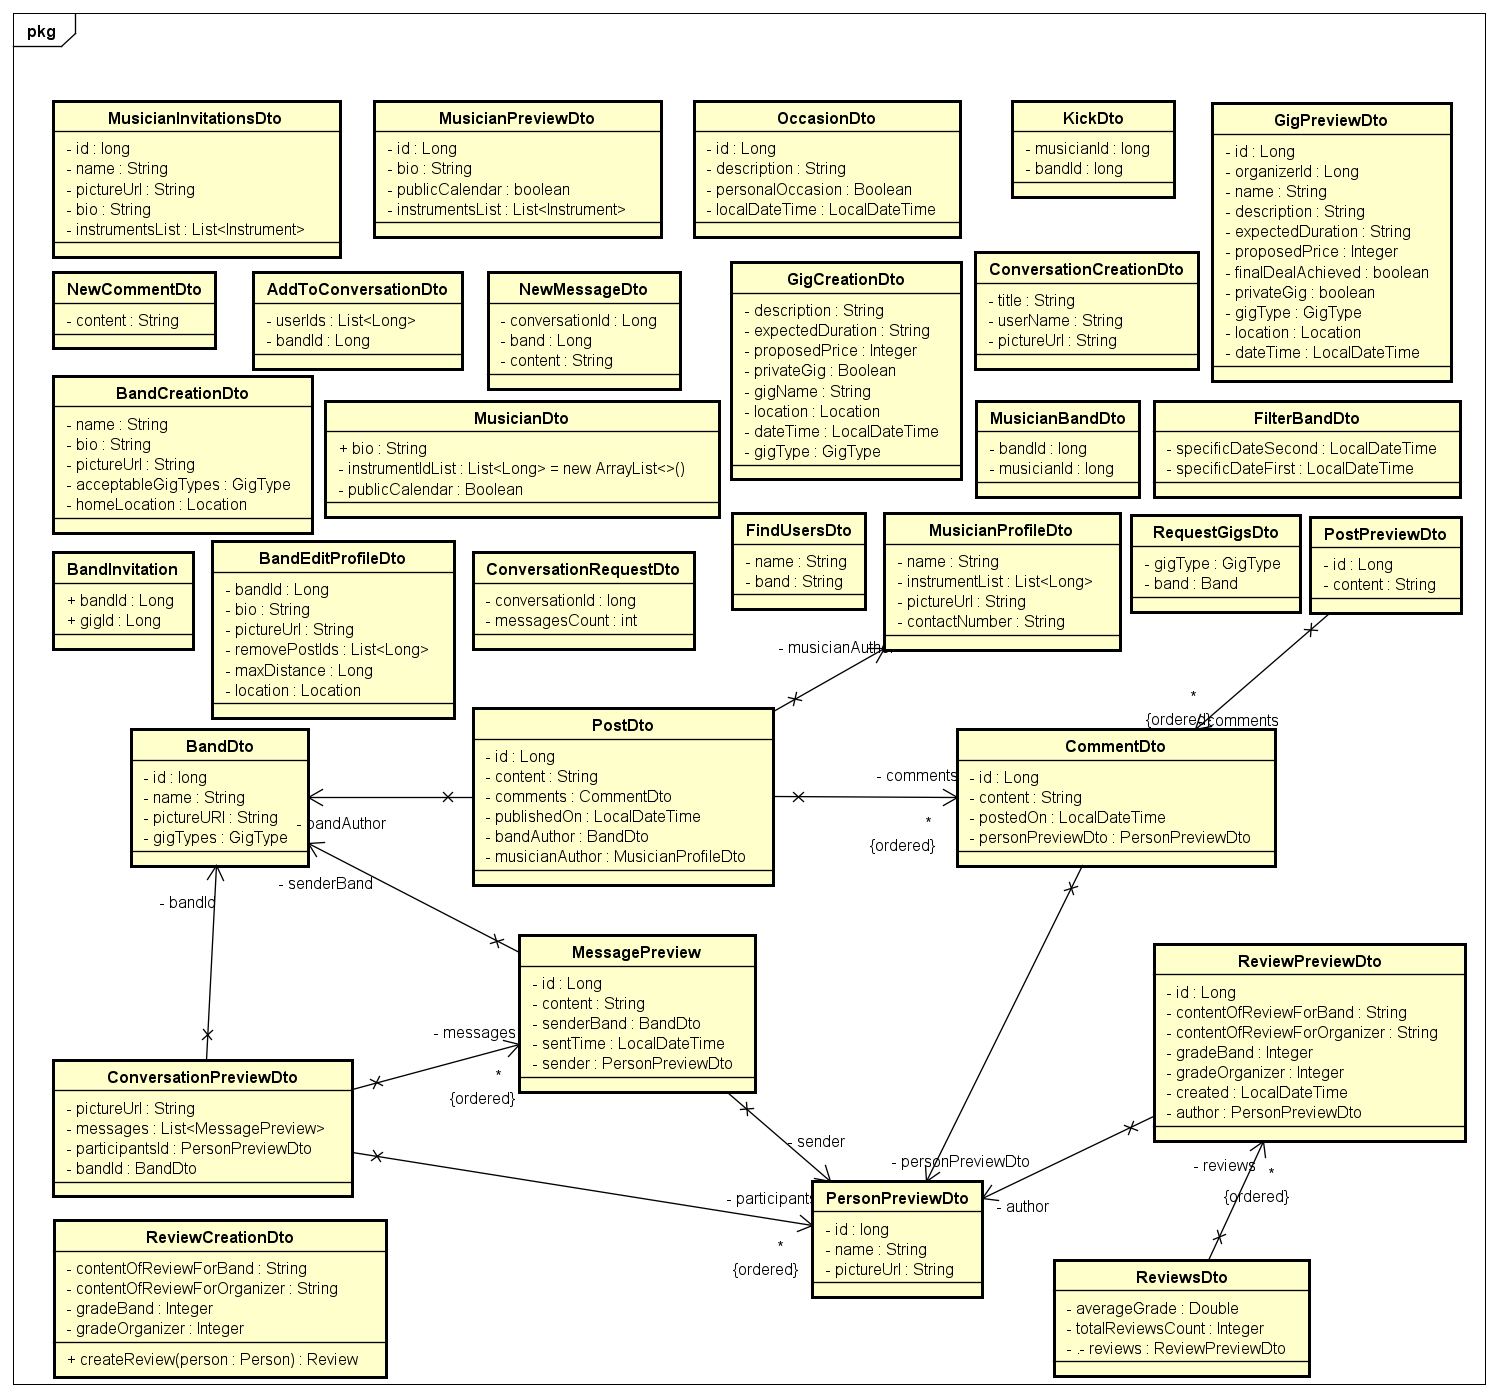
\includegraphics[width=17cm]{slike/pravi_dto2.PNG}
				\end{center}
				\caption{Dijagram razreda - dio Data transfer objects}
				\label{fig:dto}
			\end{figure}
		
		Slika 4.5 prikazuje dijagram razreda servisnog sloja. Servisi komuniciraju s repozitorijima koji pristupaju bazi i Controller-ima od kojih dobivaju i kojima vraćaju podatke. Servisi iz baze dobivaju instance objekata koji mogu biti povezani s drugim podatcima, itd. i njihov je cilj poštivajući poslovnu logiku obraditi te podatke i kao rezultat svog izvođenja vraćaju DTO-ove. Servisi sadrže svu poslovnu logiku. Gotovo svaki Controller ima pripadajući servis, a svaki je servis logički objedinjen skup funkcija poslovne logike. Iznimke koje se bacaju u servisima omataju se GigerException-om koji nasljeđuje RuntimeException. Ako se pogreška propagira iz sustava, možemo provjeriti njezin tip te ako je zamotana u GigerException, znači da je to iznimka koju smo očekivali, u protivnom je došlo do neočekivane situacije u sustavu.
		
		\begin{figure}[H]
			\begin{center}
				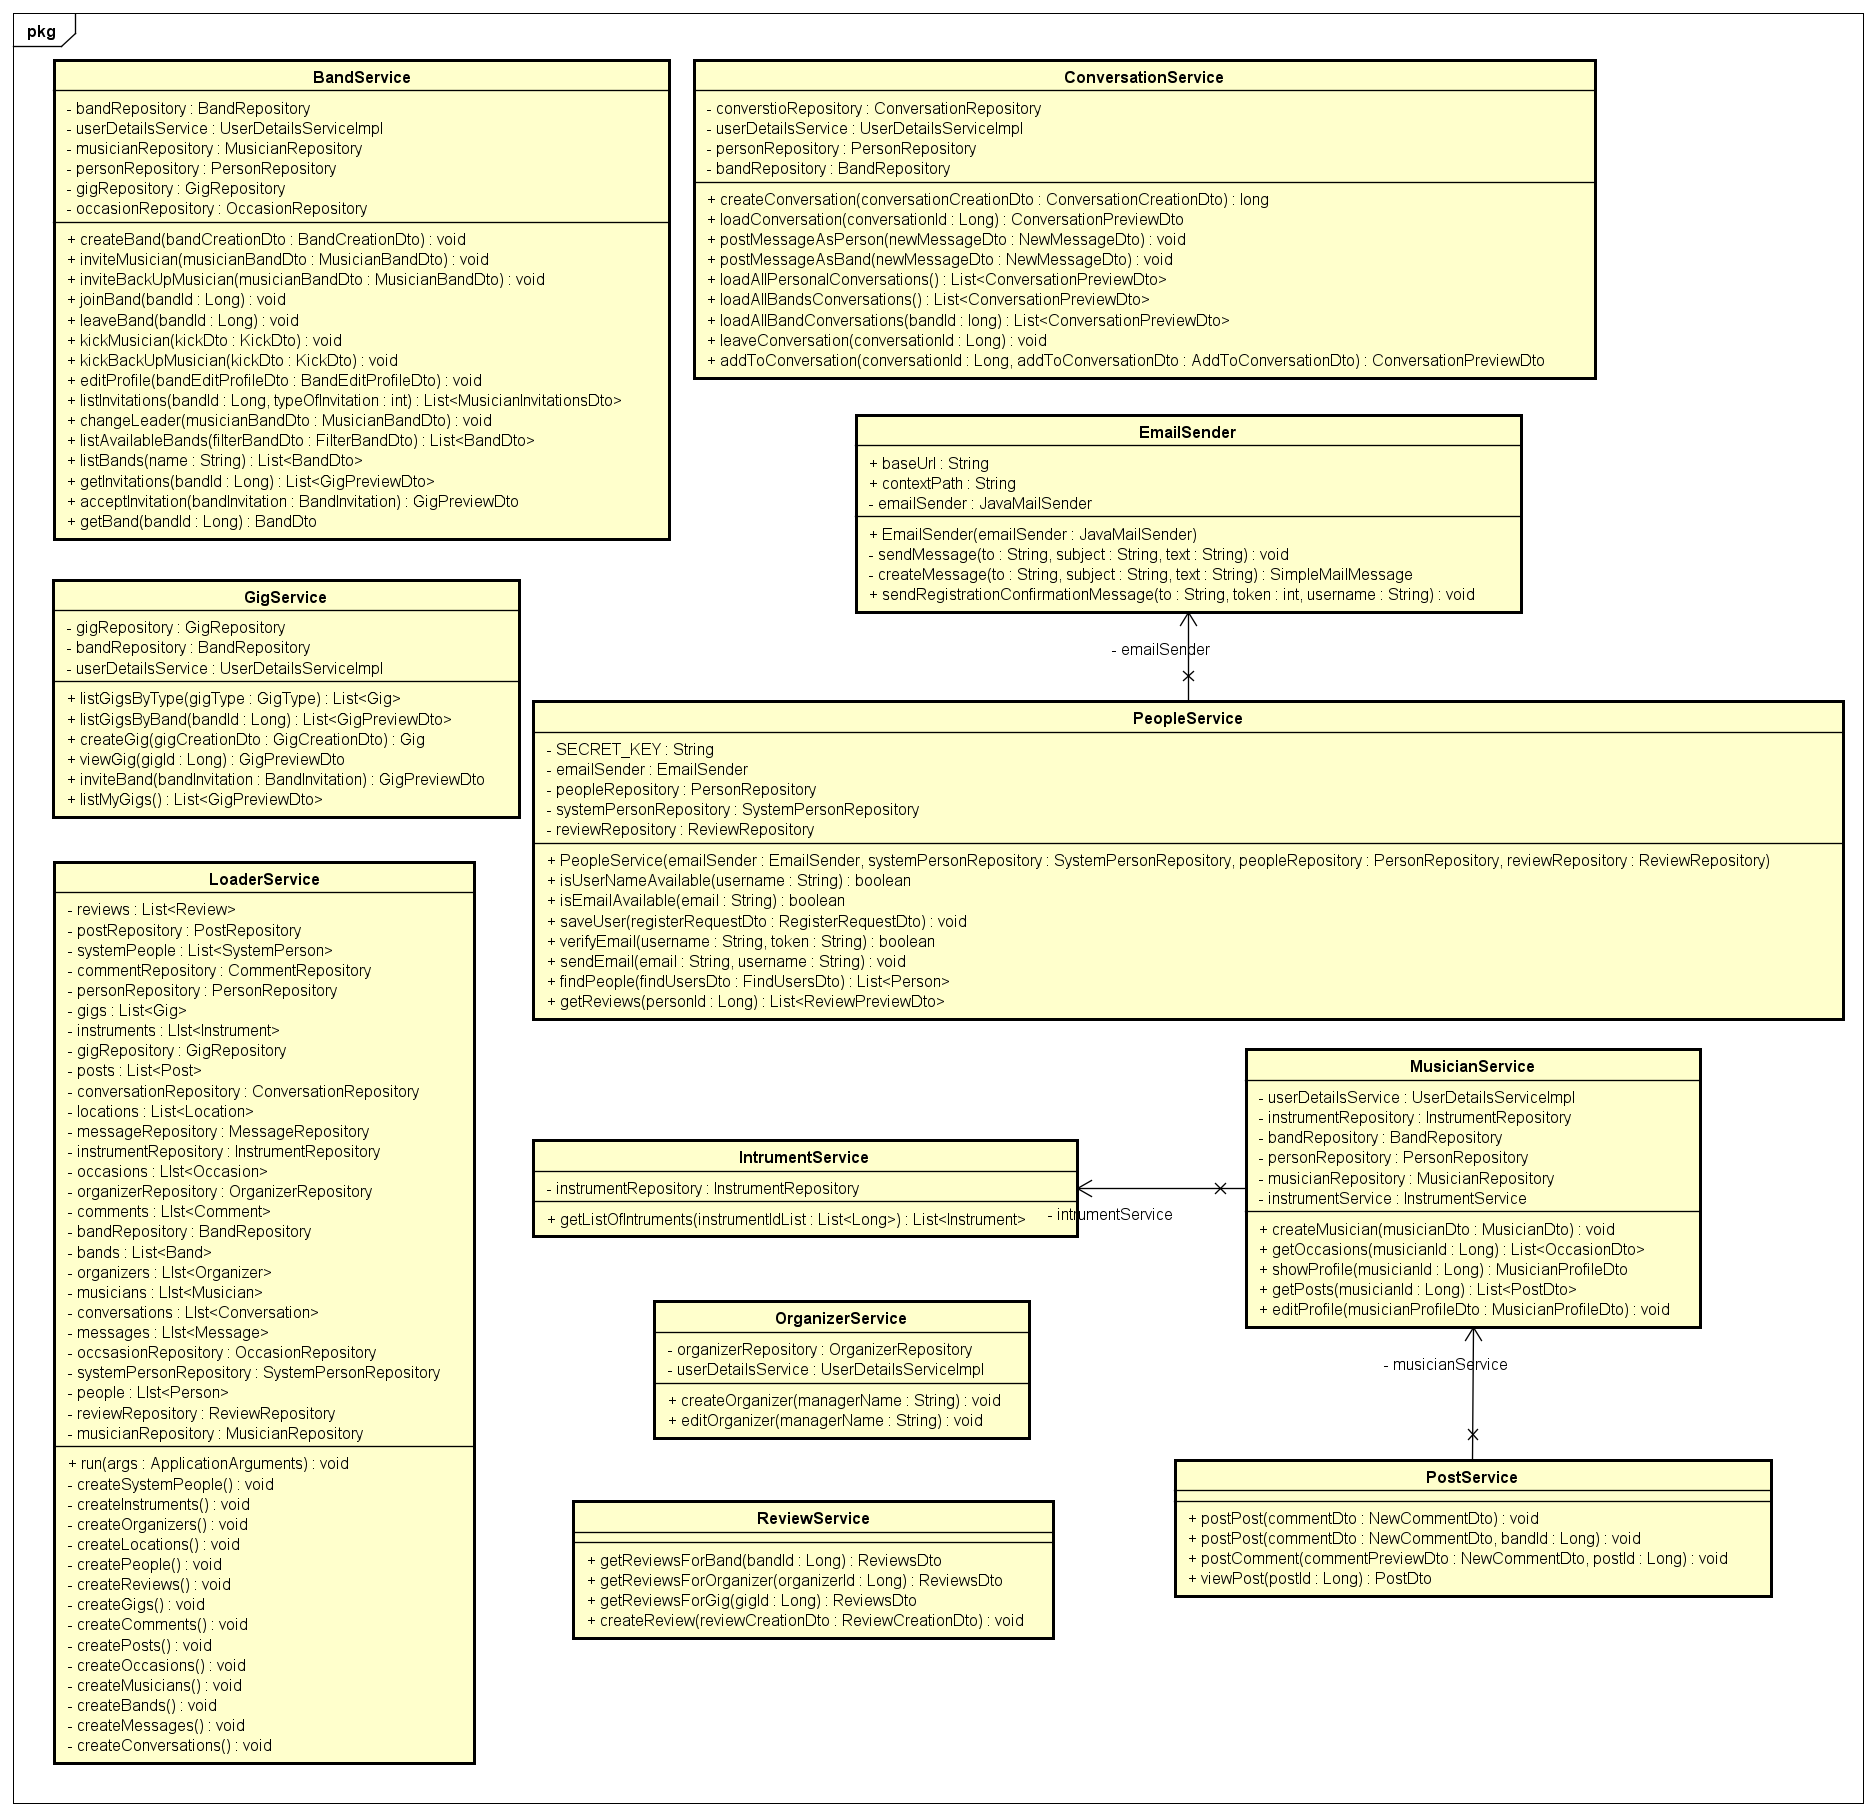
\includegraphics[width=16cm]{slike/service.PNG}
			\end{center}
			\caption{Dijagram razreda - dio Service}
			\label{fig:service}
		\end{figure}
	
	
	Slika 4.6 prikazuje razrede koji predstavljaju enitete enitetsko -  relacijskog modela u bazi podataka. Razred Band predstavlja bend kojim upravlja glazbenik koji je postavljen za voditelja benda. Razred SystemPerson predstavlja razred u kojem su objedinjeni svi sustavski podaci vezani za osobu kao što su: email, hash lozinke i id. Gig predstavlja  nastup nekog benda koji organizira određeni organizator i pri tom enkapsulira sve logističke informacije o tom nastupu. Razred Conversation omogućuje komunikaciju između aktora glazbenika i organizatora.
	Glazbenik je opisan razredom Musician, dok je organizator opisan razredom Organizer. Razredi Post, Comment, Location, Instrument, Message služe za enkapsulaciju informacija kako bi dopunili razrede poput Band, Conversation i Musician. GigType i Role predstavljaju enumeracije.
	
	
		\begin{figure}[H]
			\begin{center}
				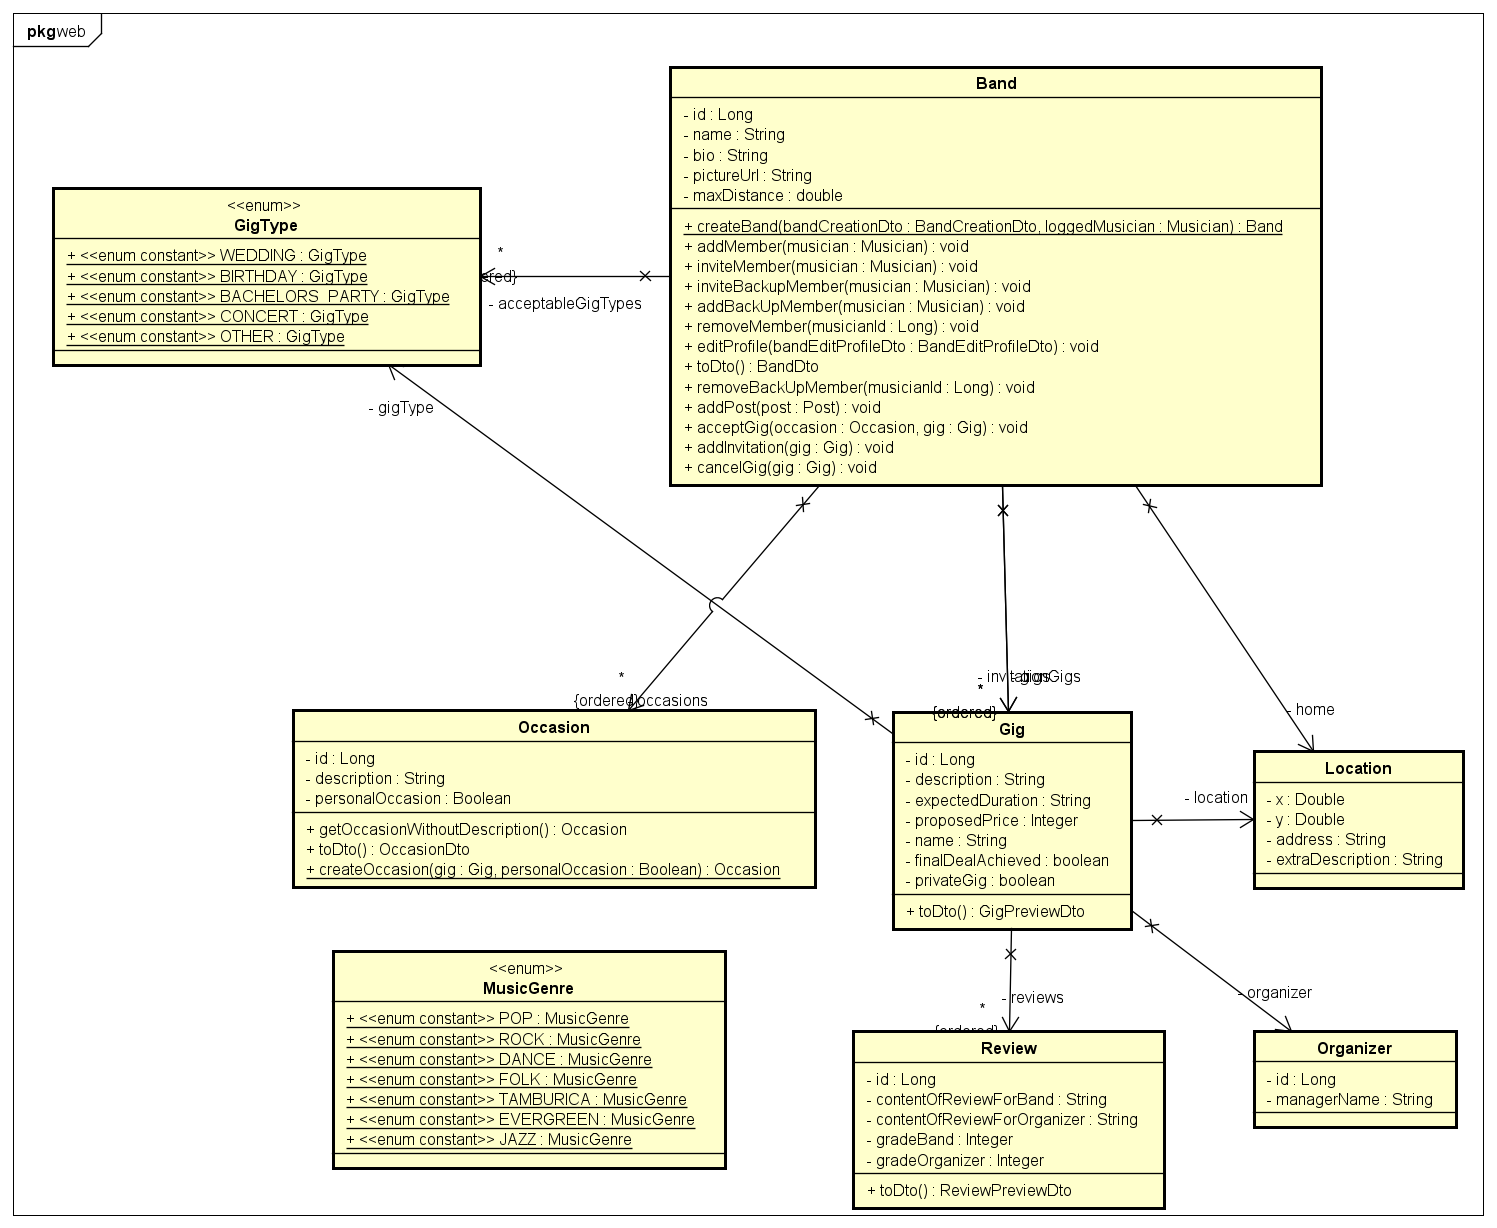
\includegraphics[width=17cm]{slike/entiteti_1.PNG}
			\end{center}
			\caption{Dijagram razreda - razredi entiteta 1}
			\label{fig:domena}
		\end{figure}
	
		\begin{figure}[H]
		\begin{center}
			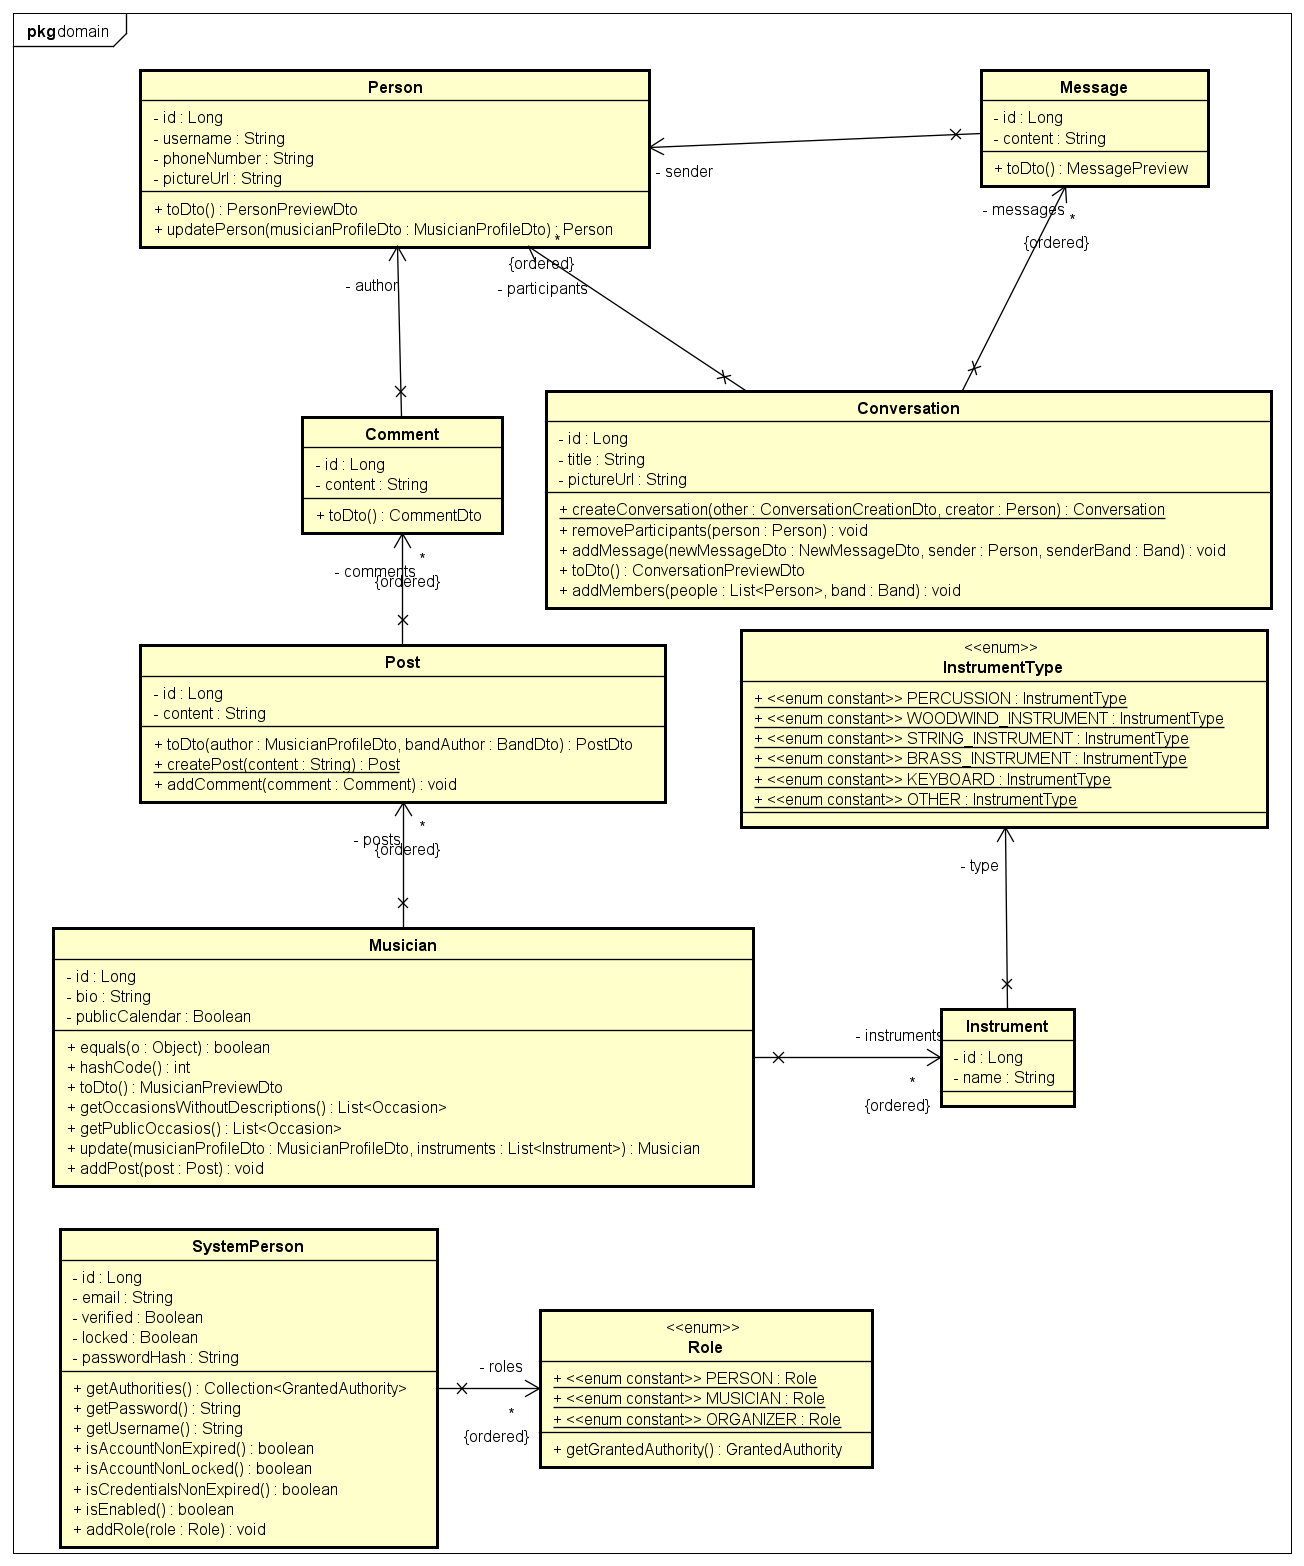
\includegraphics[width=17cm]{slike/entiteti_2.PNG}
		\end{center}
		\caption{Dijagram razreda - razredi entiteta 2}
		\label{fig:domena2}
	\end{figure}
	
	Na slici 4.7 prikazan je dijagram razreda zaduženih za Spring Security.
	Ulazna točka za autorizaciju zahtjeva je definirana u JwtRequestFilteru koji poziva UserDetailsServiceImpl da provjeri postoji li u bazi podataka zapis s akreditacijama koje se dekodiraju iz jwt tokena.
	AuthenticateController je zadužen za pružanje jwt tokena ukoliko u bazi pronađe zapis s odgovarajućim vrijednostima.
	Aplikacija ne pamti sesiju niti stanje (STATELESS) tako da korisnik prilikom postavljanja zahtjeva mora dostaviti svoj jwt token putem kojeg se autentificira i autorizira.
	JwtUtil klasa je puna pomoćnih metoda za baratanje jwt tokenom, a UserDetailsServiceImpl je posrednik između baze korisnika i AuthenticateControllera.
	Vezano uz autorizaciju, modelirana su tri DTO objekta koji definiraju objekte koje backend prima i daje kao zahtjev ili odgovor.
	

		\begin{figure}[H]
			\begin{center}
				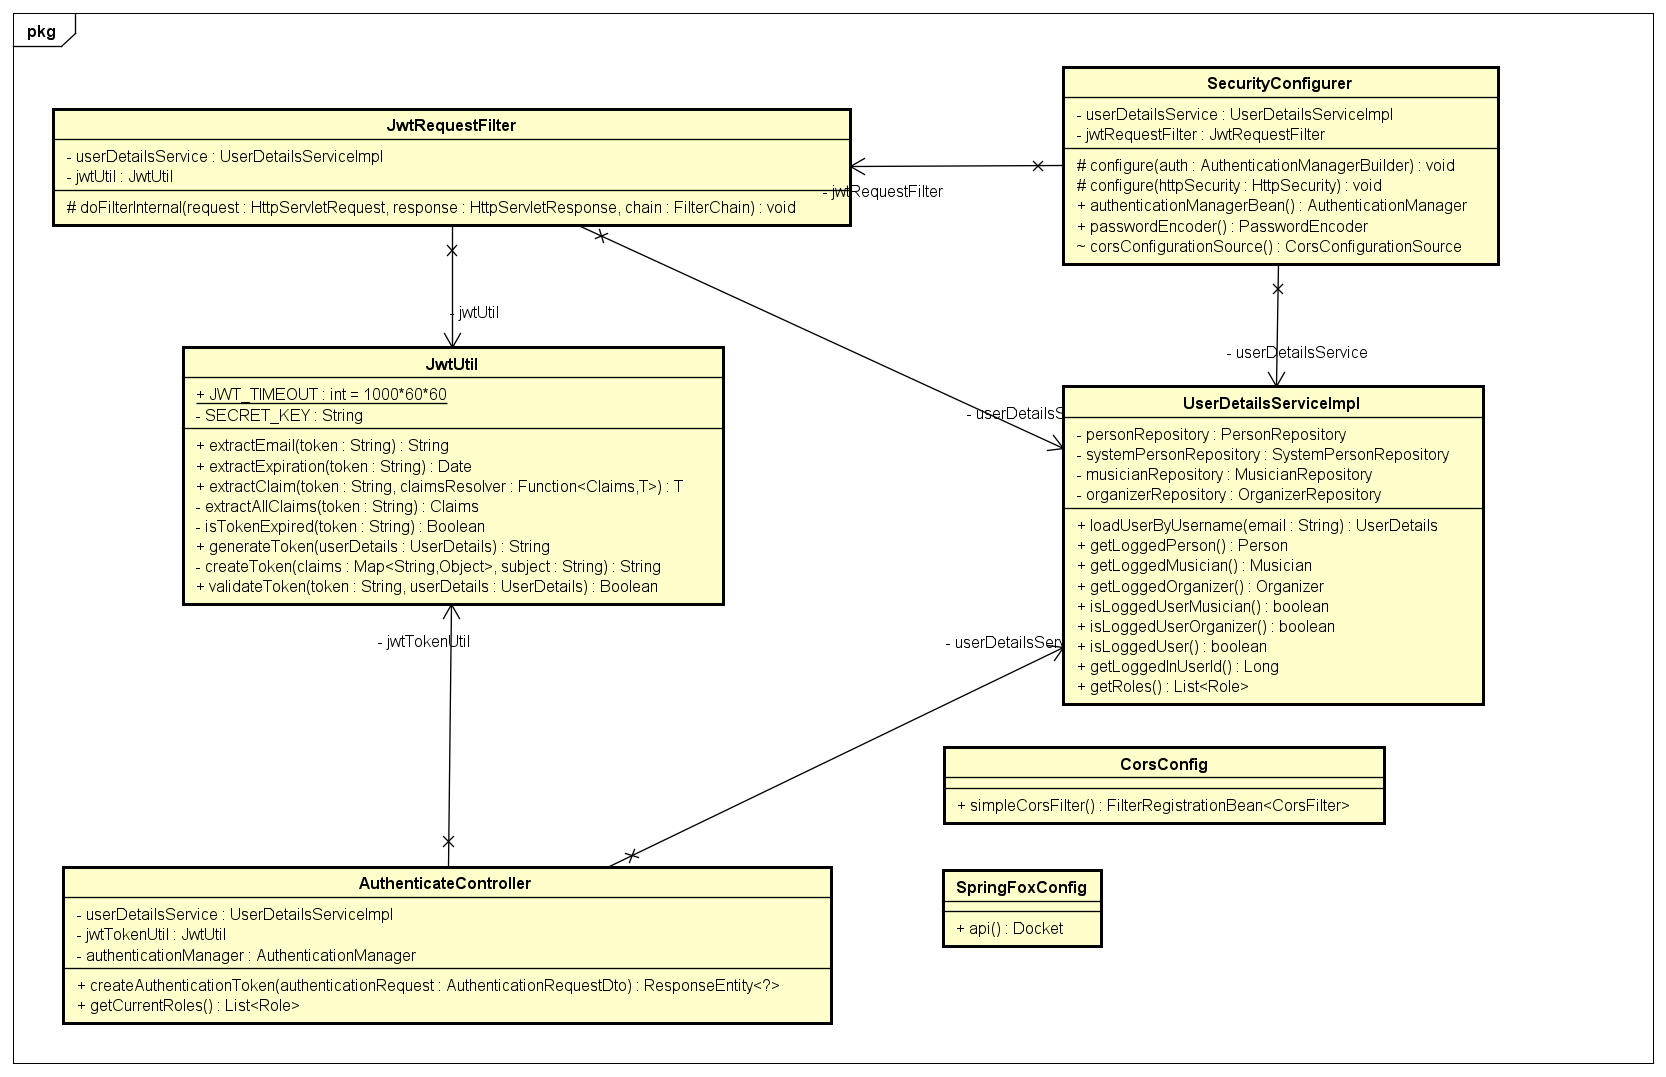
\includegraphics[width=17cm]{slike/security1.PNG}
			\end{center}
			\caption{Dijagram razreda - security}
			\label{fig:sec}
		\end{figure}
	
	Za dohvat podataka iz baze podataka koristimo Jakarta Persistence. Jakarta persistence je specifikacija programskog sučelja Java aplikacije koja opisuje upravljanje relacijskim podacima u aplikaciji. U ovoj aplikaciji za svaki entitet definiran je zasebni repozitorij koji nasljeđuje JpaRepositoryj. Jpa Repository sadrži osnovne metode za dohvat podataka, a Spring Boot omogućuje programeru da specificiranjem samo imena metode dobije implementaciju iste na korištenje. 
	
		\begin{figure}[H]
			\begin{center}
				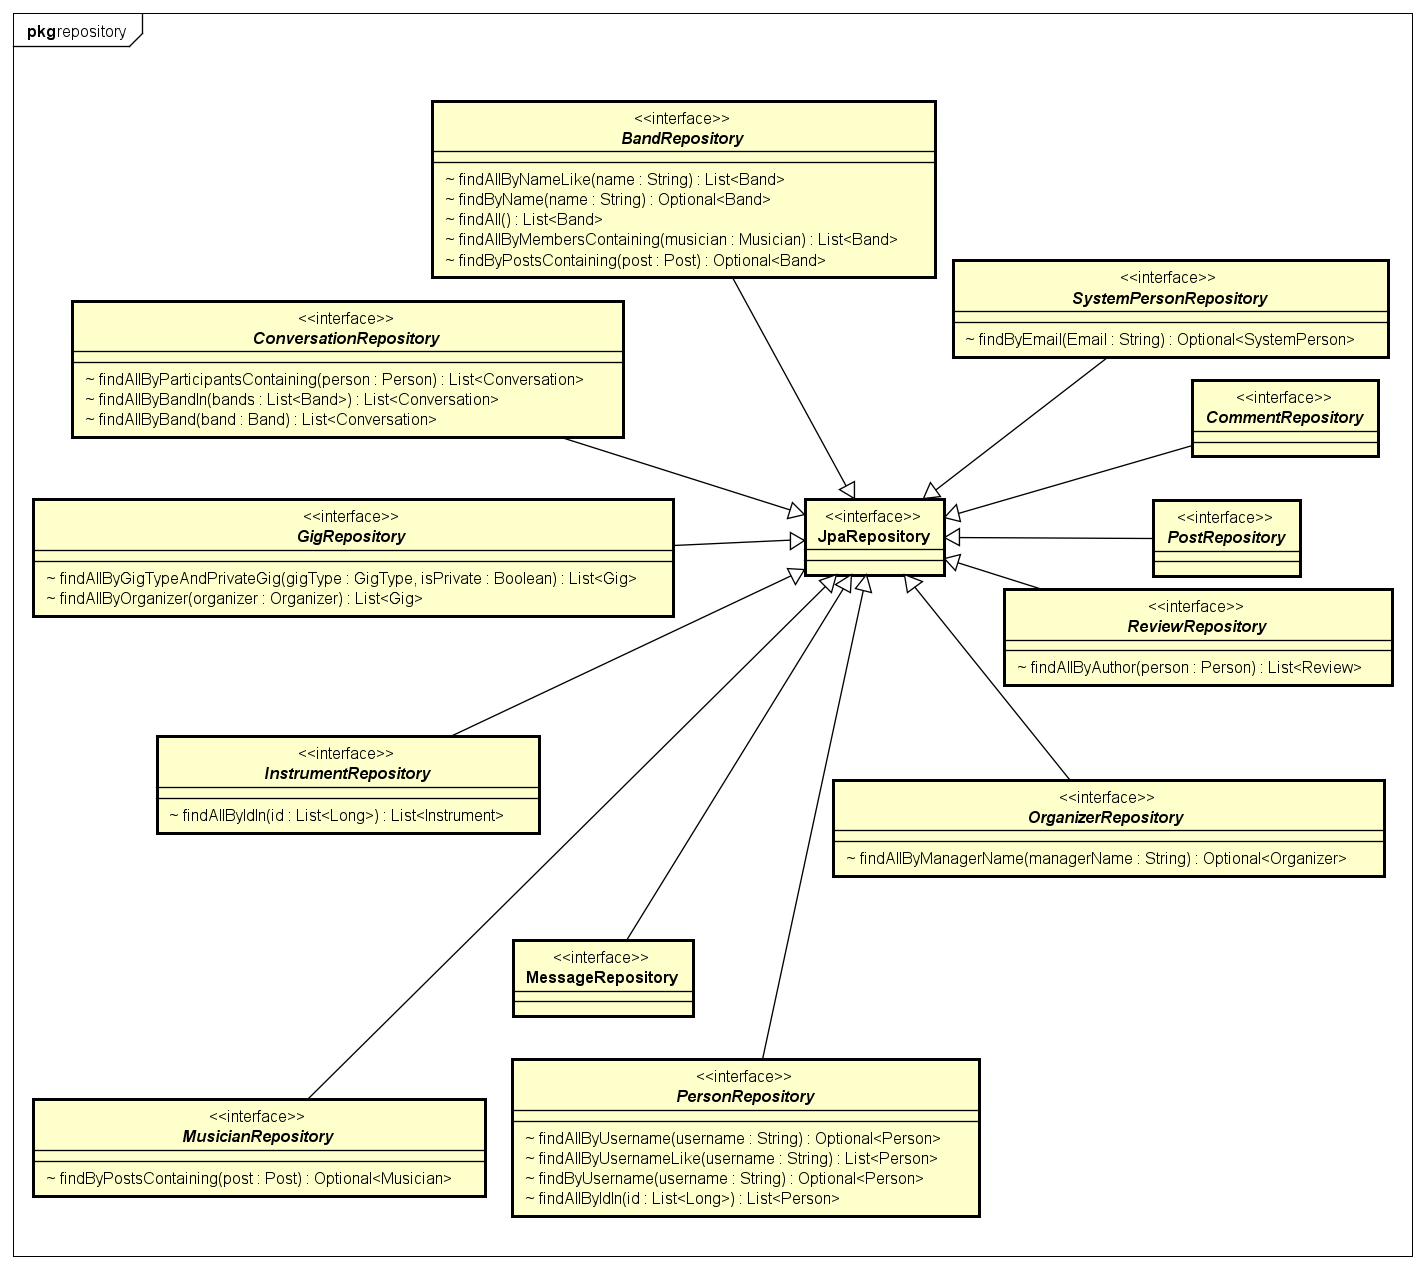
\includegraphics[width=17cm]{slike/repository1.PNG}
			\end{center}
			\caption{Dijagram repozitorija - repository}
			\label{fig:repository}
		\end{figure}
	
	Ovim dijagramom prikazane su moguće pogreške kao i iznimke. Pogreške se u ovom slučaju nalaze u Enumu Errorcode i služe za zaustavljanje operacija čijim izvođenjem se krši pravo pristupa ili se pokušava izvesti nemoguća akcija. Sve ostale logičke iznimke omotavaju se u iznimu GigerException. Za reprezentacijsko stanje prijenosa uvedena je iznimka RestExceptionHandler.
		
		\begin{figure}[H]
			\begin{center}
				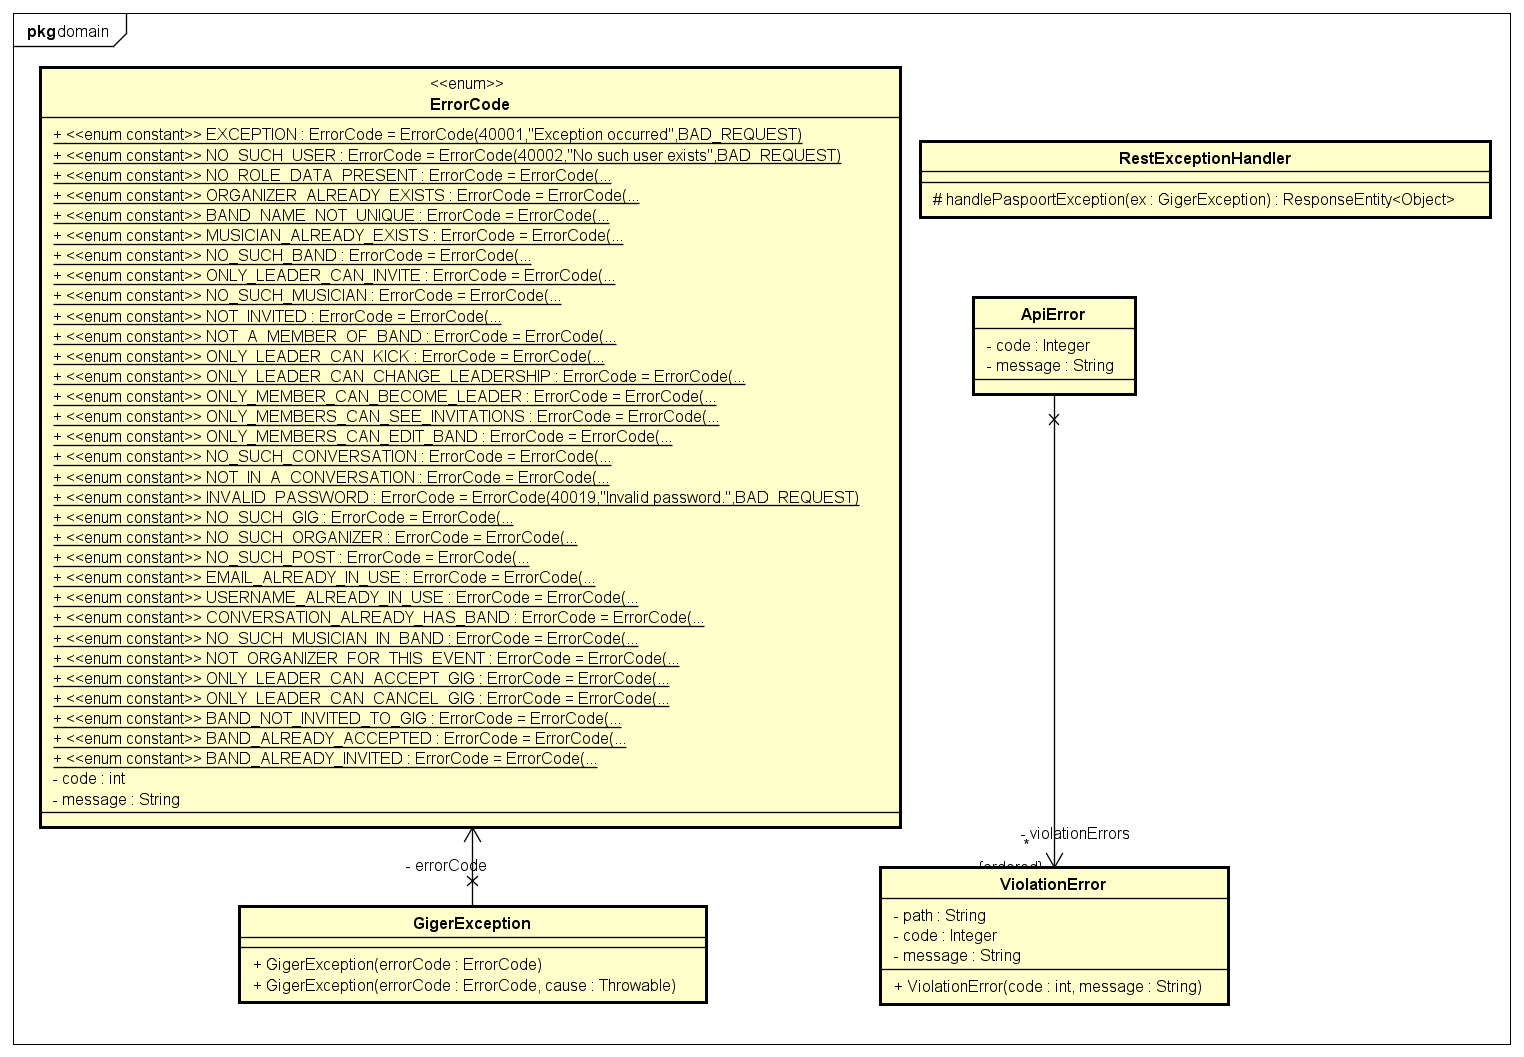
\includegraphics[width=17cm]{slike/errors1.PNG}
			\end{center}
			\caption{Dijagram razreda - errors}
			\label{fig:err}
		\end{figure}
	
		
	
	
	\eject
	
	\section{Dijagram stanja}
	
    Sljedeći dijagram stanja prikazuje stvaranje giga.Nakon uspješnog stvaranja giga, isti i dalje nije viđen pod opcijom "View public gigs". Da bi ostali korisnici mogli vidjeti taj gig, on prvo mora biti finaliziran.To znači da  organizator mora pozvati bend u svoj gig te nakon  što bend prihvati nastup ,gig postaje finaliziran (javan).
	
	
	
	
		\begin{figure}[H]
			\begin{center}
				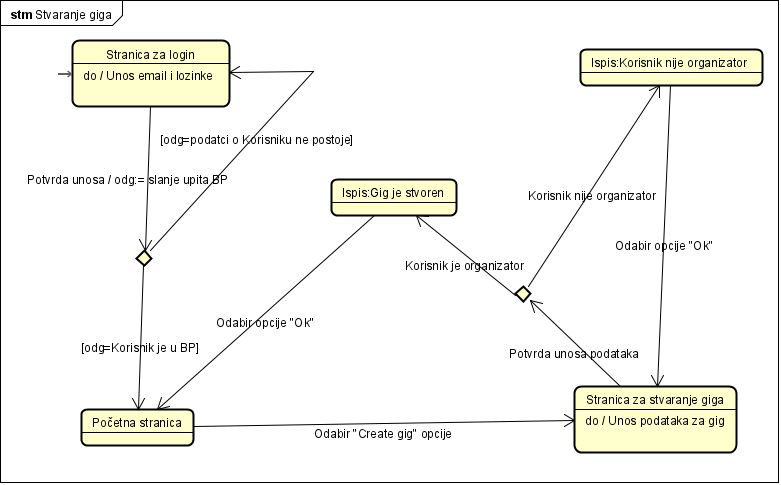
\includegraphics[width=17cm]{slike/stmStvaranjGiga.JPG}
			\end{center}
			\caption{Dijagram stanja - stvaranje giga}
			\label{fig:stm}
		\end{figure}
	
	\eject
	
	
	\section{Dijagram aktivnosti}
	
	\textit{\textbf{dio 2. revizije}} \\
	
	\textit{Potrebno je priložiti dijagram aktivnosti s pripadajućim opisom. Dijagram aktivnosti treba prikazivati značajan dio sustava.} \\
	
	
	\eject
	
	
	
	\section{Dijagram komponenti}
	
	\textit{\textbf{dio 2. revizije}} \\
	
	\textit{Potrebno je priložiti dijagram komponenti s pripadajućim opisom. Dijagram komponenti treba prikazivati strukturu cijele aplikacije.} \\
	
	\eject	

	\chapter{Implementacija i korisničko sučelje}
		
		
		\section{Korištene tehnologije i alati}
		
			\textbf{\textit{dio 2. revizije}} \\
			
			 \textit{Detaljno navesti sve tehnologije i alate koji su primijenjeni pri izradi dokumentacije i aplikacije. Ukratko ih opisati, te navesti njihovo značenje i mjesto primjene. Za svaki navedeni alat i tehnologiju je potrebno \textbf{navesti internet poveznicu} gdje se mogu preuzeti ili više saznati o njima}.
			

    	
        \begin{longtabu} to \textwidth {|X[6, l+3]|X[25, 1]|X[20, 2]|}
		
    		\hline \multicolumn{3}{|c|}{\textbf{Backend}}	 \\[3pt] \hline
    		\endfirsthead
    		
    		\hline
    		\endlastfoot
    		
    		PostgreSQL & \href{https://www.postgresql.org/}{https://www.postgresql.org/}	& Objektno-relacijska baza podataka 	\\ \hline
    		Java 11 & \href{https://www.oracle.com/technetwork/java/javase/downloads/jdk11-downloads-5066655.html}{https://www.oracle.com} & Programski jezik u kojem je napisan backend dio aplikacije	\\ \hline
    		Java Spring Boot & \href{https://spring.io/projects/spring-boot}{https://spring.io/projects/spring-boot} & Razvojni okvir 	\\ \hline
    		
    		Spring Web MVC  & \href{https://docs.spring.io/spring/docs/current/spring-framework-reference/web.html}{https://docs.spring.io/spring/} & Web framework za rukovanje zahtjevima 	\\ \hline
    		Spring Security  & \href{https://spring.io/projects/spring-security}{https://spring.io/projects/spring-security} & 
Moćan i vrlo prilagodljiv okvir za provjeru autentičnosti i kontrolu pristupa 	\\ \hline

        Lombok  & \href{https://projectlombok.org/}{https://projectlombok.org/} & Java library za pregledniji kod 	\\ \hline
    	\end{longtabu}
			
			

			\eject
			
        \begin{longtabu} to \textwidth {|X[4, l+3]|X[25, l]|X[20, 2]|}
		
    		\hline \multicolumn{3}{|c|}{\textbf{Frontend}}	 \\[3pt] \hline
    		\endfirsthead
    		
    		\hline
    		\endlastfoot
    		
    		React & \href{https://reactjs.org/}{https://reactjs.org/}	& JavaScript library za izgradnju sučelja	\\ \hline
    		Ant Design & \href{https://ant.design/}{https://ant.design/} & Design library sa komponentama za lakšu izgradnju korisničkog sučelja	\\ \hline
    		
    		NPM & \href{https://www.npmjs.com/}{https://www.npmjs.com/} & Upravitelj paketa za programski jezik JavasScript	\\ \hline
    		
    		OpenCage Geocoder & \href{https://opencagedata.com/}{https://opencagedata.com/} & API za dohvaćanje koordinata iz adrese	\\ \hline
    	\end{longtabu}			
			
			
        \begin{longtabu} to \textwidth {|X[4, l+3]|X[25, l]|X[20, 2]|}
		
    		\hline \multicolumn{3}{|c|}{\textbf{Komunikacija}}	 \\[3pt] \hline
    		\endfirsthead
    		
    		\hline
    		\endlastfoot
    		
    		Slack & \href{https://slack.com/intl/en-hr/}{https://slack.com/intl/en-hr/}	& Platforma koju smo koristili za lakšu komunikaciju	\\ \hline
    		Trello & \href{https://trello.com/en}{https://trello.com/en} & Alat koji nam je olakšao zajedniči rad i raspoređivanje  projektnih zadataka	\\ \hline
    	\end{longtabu}
    
        \eject
			
			
			
		
	
		\section{Ispitivanje programskog rješenja}
	
			
			\subsection{Ispitivanje komponenti}
			\textit{Potrebno je provesti ispitivanje jedinica (engl. unit testing) nad razredima koji implementiraju temeljne funkcionalnosti. Razraditi \textbf{minimalno 6 ispitnih slučajeva} u kojima će se ispitati redovni slučajevi, rubni uvjeti te izazivanje pogreške (engl. exception throwing). Poželjno je stvoriti i ispitni slučaj koji koristi funkcionalnosti koje nisu implementirane. Potrebno je priložiti izvorni kôd svih ispitnih slučajeva te prikaz rezultata izvođenja ispita u razvojnom okruženju (prolaz/pad ispita). }
			
			
			
			Da bismo testirali backend, napravili smo dvije vrste testova. JUnit testove za testiranje servisa te integracijske testove koje je najlakše opisati kao automatizirane Postman zahtjeve.
			
			Servisi su testirani na način da ih gledamo kao crne kutije koje za određeni ulaz trebaju odraditi određene akcije ili vratiti određene objekte. Nomenklatura testovi servisa (BandServiceTest) slijedi pravilo given\_when\_then. Naprimjer, ako testiramo metodu naziva createMusician, pretpostavljajuci da on još ne postoji i očekujući da se kreira glazbenik u bazi, naziv testa bio bi 
			noSuchMusician\_
			createMusician\_createAndPersistateMusician().
			
			Pomoću Mockito frameworka u testovima mockamo (oponašamo) ulaze te na taj način kontroliramo ulaze i okolinu metode koju testiramo. Drugim riječima, kada radimo test za neku komponentu ili servis, pretpostavljamo da su svi ulazi dobri i ne zanima nas utjecaj naše komponente na drugu komponentu, već samo direktni izlaz. Na taj način dobivamo testove koji su međusobno nepovezani i koji definiraju željeno ponašanje aplikacije. Ukoliko u daljnjem razvoju neki od razvojnih programera promijeni neko ponašanje koje ima utjecaj na druge komponente, pravilno napisani testovi trebali bi pasti i upozoriti ga da će se njegova promjena propagirati dublje u aplikaciju. Testovi koji su pisani ciljano na pojedine komponente sustava u kontroliranim uvjetima prilikom izvođenja precizno ukazuju na vjerojatan izvor pogreške. Na primjer, ako promijenimo implementaciju kreiranja glazbenika te on u trenutku kreiranja ne dobije id, samo testovi koji provjeravaju parametre nakon inicijalizacije bi trebali pasti, a ne svi testovi koji se u nekom trenutku pozivaju na tu funkcionalnost.
			
			Svaki napisan test odijeljen je u tri cjeline, a to su Arrange, Act, Assert. U prvom dijelu uređujemo i mockamo ulaze u testirajuću komponentu, na prije opisan način. U drugom dijelu testa poziva se akcija ili niz akcija čije djelovanje želimo provjeriti, a u trećem dijelu testa provjeravamo jesu li posljedice izvršavanja drugoga dijela testa u skladu s očekivanjima.
			
			Na slici 5.1 nalazi se primjer unit testa. Linije 380-399 su Arrange, linija 401 je Act, dok su linije 404-408 Assert dio testa.
			
			\begin{figure}[H]
				\begin{center}
					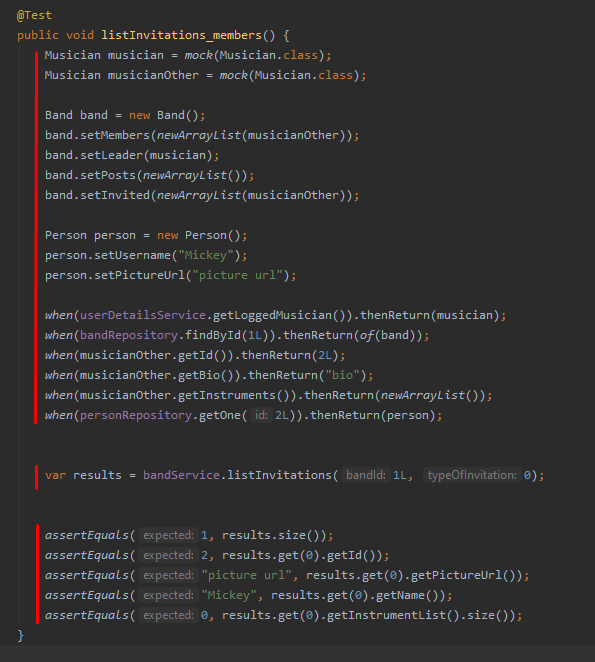
\includegraphics[width=13cm]{slike/junit_test.PNG}
				\end{center}
				\caption{Primjer JUnit testa}
				\label{fig:junit}
			\end{figure}
		
			
			Pošto je pisanje testova često i iscrpnije od pisanja implementacije (BandService ima 210 linija koda, dok BandServiceTest koji ni ne testira baš sve metode u njemu ima 558), za ovaj projekt nismo radili TDD (test driven development) već smo naknadno radili testove za postojeću implementaciju kako bismo potvrdili implementaciju i programski dokumentirali očekivano ponašanje.
			
			Uz dodatak BandService testovima postoji i nekoliko testova u EmailSenderTest koji pokazuju kako testirati komponentu čiju implementaciju ne znamo.
			
			
			Uz tridesetak JUnit testova čija je glavna prednost brzo izvođenje, napisali smo desetak integracijskih testova. Kao što smo već spomenuli, integracijski testovi slični su ručnom pregledavanju u Postmanu. Svaki integracijski test pokreće aplikaciju ispočetka tako da su mu stanje baze i aplikacije (kontekst) jednaki kao kad se pokrene aplikacija. U ovim testovima koristimo MockMvc kako bismo simulirali http request kojemu moramo odrediti metodu (GET, POST) te dodati pripadajuća zaglavlja. U ovom testu verificiramo je li ono što je vratila metoda jednako onome što se očekivalo (najčešće usporedbe DTO-ova).
			
			\begin{figure}[H]
				\begin{center}
					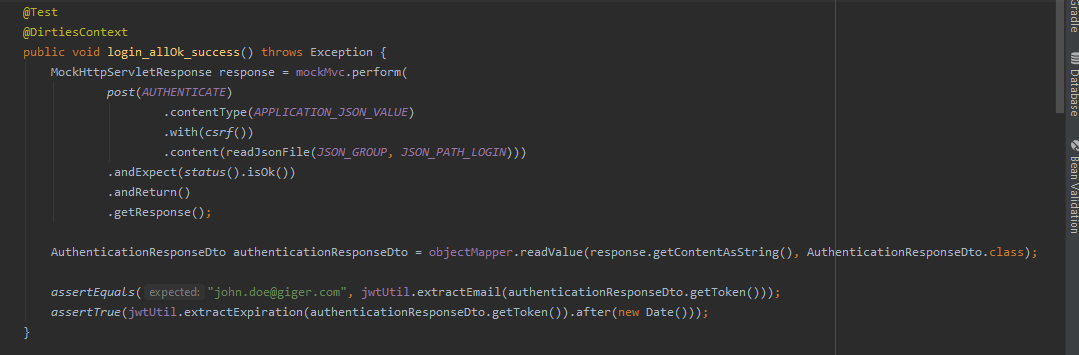
\includegraphics[width=17cm]{slike/integracijski_test.PNG}
				\end{center}
				\caption{Primjer integracijskog testa}
				\label{fig:inttest}
			\end{figure}
			
			Tehnike testiranja programske potpore nadahnute su knjigom Test-Driven Development Kenta Becka.
			
			
			
			\subsection{Ispitivanje sustava}
			
			 \textit{Potrebno je provesti i opisati ispitivanje sustava koristeći radni okvir Selenium\footnote{\url{https://www.seleniumhq.org/}}. Razraditi \textbf{minimalno 4 ispitna slučaja} u kojima će se ispitati redovni slučajevi, rubni uvjeti te poziv funkcionalnosti koja nije implementirana/izaziva pogrešku kako bi se vidjelo na koji način sustav reagira kada nešto nije u potpunosti ostvareno. Ispitni slučaj se treba sastojati od ulaza (npr. korisničko ime i lozinka), očekivanog izlaza ili rezultata, koraka ispitivanja i dobivenog izlaza ili rezultata.\\ }
			 
			 \textit{Izradu ispitnih slučajeva pomoću radnog okvira Selenium moguće je provesti pomoću jednog od sljedeća dva alata:}
			 \begin{itemize}
			 	\item \textit{dodatak za preglednik \textbf{Selenium IDE} - snimanje korisnikovih akcija radi automatskog ponavljanja ispita	}
			 	\item \textit{\textbf{Selenium WebDriver} - podrška za pisanje ispita u jezicima Java, C\#, PHP koristeći posebno programsko sučelje.}
			 \end{itemize}
		 	\textit{Detalji o korištenju alata Selenium bit će prikazani na posebnom predavanju tijekom semestra.}
			
			\eject 
		
		
		\section{Dijagram razmještaja}
			 
			 Dijagrami razmještaja opisuju topologiju sklopovlja i programsku potporu koja se koristi u implementaciji sustava u njegovom radnom okruženju. Sve komponente programske potpore smještene su na oblak platformu Heroku. Heroku kao platforma omogućuje programerima izvođenje i operiranje nad aplikacijama u oblaku. U ovome slučaju pozadinska i prednja aplikacija razmještene su na zasebene poslužitelje kao i baza podataka. Sustav je baziran na arhitekturi klijent - poslužitelj i komunikacija između njih odvija se HTTP protokolom. 
			 
			 	\begin{figure}[H]
			 	\begin{center}
			 		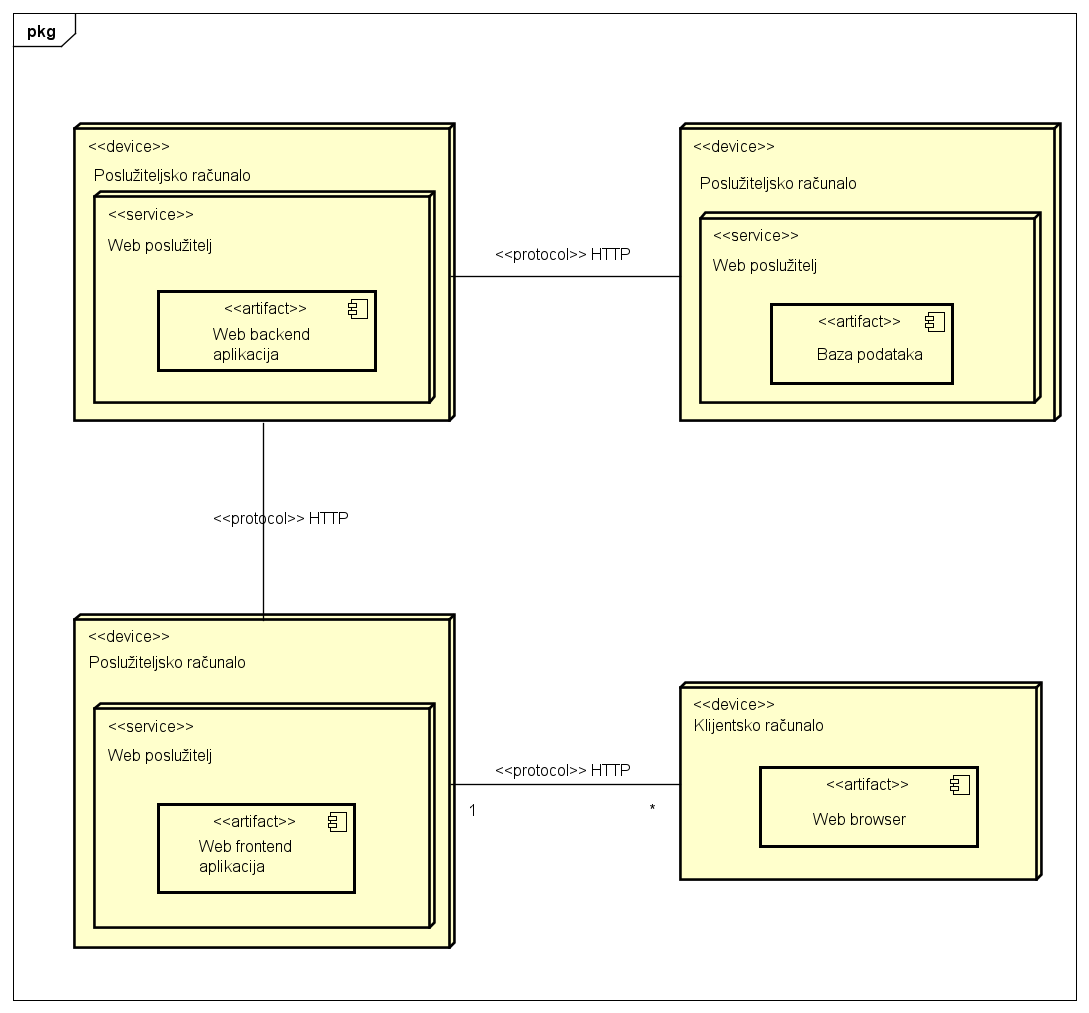
\includegraphics[width=15cm]{slike/deploy_fin.PNG}
			 	\end{center}
			 	\caption{Dijagram razmještaja}
			 	\label{fig:deploy_pic}
			 \end{figure}
			
			\eject 
		
		\section{Upute za puštanje u pogon}
			
			
			Ponajprije je potrebno preuzeti Postgres SQL bazu podataka na operacijski sustav, poželjno Windows. Nakon toga je potrebno provesti standardnu instalaciju. U servisu LoaderService nalaze se testni podaci za inicijalno punjenje baze. Za postavljanje lozinke baze potrebno je je u password polje u system-local.properties postaviti prethodno definiranu lozinku za bazu podataka. Alternativno moguće je u root direktoriju standardnog terminala  pokrenuti naredbu docker-compose up koja će u virtualnom kontejneru pokrenuti servise koji su predefinirani u dockeru docker-compose.yml datoteci. Za konfiguraciju aplikacije na Heroku poslužitelju koristi se system.properties iz kojeg se čita pokretanje Spring Boot aplikacije defaultnim profilom.
			U izradi aplikacije korišten je radni okvir Spring Boot. Za pokretanje Javine aplikacije
			potrebno je imati instaliran Java Runtime Environment v11. Za pokretanje frontend aplikacije
			potrebno je imati instaliranu platformu Node.js. Za pokretanje također je potrebno otpakirati 
			arhivu server.var. Kako bi se pokrenuo build koristi se automatizirani sustav Gradle. 
			
			\eject 
	\label{key}\chapter{Zaključak i budući rad}
		
		\textbf{\textit{dio 2. revizije}}\\
		
		 \textit{U ovom poglavlju potrebno je napisati osvrt na vrijeme izrade projektnog zadatka, koji su tehnički izazovi prepoznati, jesu li riješeni ili kako bi mogli biti riješeni, koja su znanja stečena pri izradi projekta, koja bi znanja bila posebno potrebna za brže i kvalitetnije ostvarenje projekta i koje bi bile perspektive za nastavak rada u projektnoj grupi.}
		
		 \textit{Potrebno je točno popisati funkcionalnosti koje nisu implementirane u ostvarenoj aplikaciji.}
		
		\eject 
		
	
	\chapter*{Popis literature}
		\addcontentsline{toc}{chapter}{Popis literature}
	 	
 		\begin{enumerate}
			
			
			\item  Oblikovanje programske potpore, FER ZEMRIS, \url{http://www.fer.hr/predmet/opp}
			
			\item Astah Community, \url{http://astah.net/editions/uml-new}
			\item GitLab Pipelines, \url{https://docs.gitlab.com/ee/ci/pipelines.html}
			\item Sprint Boot, \url{https://docs.spring.io/spring-boot/docs/current-SNAPSHOT/reference/htmlsingle/}
			\item Kent Beck, \textit{Test Driven Development}, 2000.
		\end{enumerate}
		
		 
	
	
	\begingroup
	\renewcommand*\listfigurename{Indeks slika i dijagrama}
	%\renewcommand*\listtablename{Indeks tablica}
	%\let\clearpage\relax
	\listoffigures
	%\vspace{10mm}
	%\listoftables
	\endgroup
	\addcontentsline{toc}{chapter}{Indeks slika i dijagrama}


	
	\eject 
		
	\chapter*{Dodatak: Prikaz aktivnosti grupe}
		\addcontentsline{toc}{chapter}{Dodatak: Prikaz aktivnosti grupe}
		
		\section*{Dnevnik sastajanja}
		
		\begin{packed_enum}
			\item  sastanak
			
			\item[] \begin{packed_item}
				\item Datum: 3. listopada 2019.
				\item Prisutni: I. Juren, T. Krmek, M. Jurić, M. Zec, S. Gaši, M. Nosil, P. Lanča
				\item Teme sastanka:
				\begin{packed_item}
					\item  predlaganje ideja za projektni zadatak
					\item  odabir između web ili mobilne aplikacije
					\item  svaki član je iznio koja predznanja ili iskustva ima vezano za stvaranje aplikacije  
				\end{packed_item}
			\end{packed_item}
			
			\item  sastanak
			\item[] \begin{packed_item}
				\item Datum: 9. listopada 2019.
				\item Prisutni: I. Juren, T. Krmek, M. Jurić, M. Zec, S. Gaši, M. Nosil, P. Lanča
				\item Teme sastanka:
				\begin{packed_item}
					\item  upoznavanje s mentorima i demonstratorom
					\item  razgovor o tehnologijama koje ćemo koristiti
					\item  dogovoren način komunikacije s asistentom i demonstratorom
					\item  upoznavanje s ponuđenim projektom te razgovor o tome kako poboljšati naš prijedlog projekta
				\end{packed_item}
			\end{packed_item}
			
			\item  sastanak
			\item[] \begin{packed_item}
				\item Datum: 14. listopada 2019.
				\item Prisutni: I. Juren, M. Jurić, M. Zec, S. Gaši, P. Lanča
				\item Teme sastanka:
				\begin{packed_item}
					\item  sastanak s asistentom
					\item  nacrtana gruba shema različitih korisnika s pripadajućim potrebnim pristupom
					\item  predlaganje funkcionalnosti, dogovoreno što se obavezno mora implementirati 
				\end{packed_item}
			\end{packed_item}
			
			\item  sastanak
			\item[] \begin{packed_item}
				\item Datum: 22. listopada 2019.
				\item Prisutni: I. Juren, T. Krmek, M. Jurić, M. Zec, S. Gaši, M. Nosil, P. Lanča
				\item Teme sastanka:
				\begin{packed_item}
					\item  razrada must i could have funkcionalnosti
					\item  izjašnjavanje svojih nedoumica te njihovo razrješavanje, eventualno stavljene na popis za pitanja na sastanku s asistentom
					\item  razriješena problematika benda (glavni i rezervni članovi)
					\item  nakon internog, sastanak s asistentom: dogovorena detaljnija implementacija, napravljen popis zadataka koje treba odraditi do idućeg sastanka
				\end{packed_item}
			\end{packed_item}
			
			\item  sastanak
			\item[] \begin{packed_item}
				\item Datum: 28. listopada 2019.
				\item Prisutni: I. Juren, M. Jurić, M. Zec, S. Gaši, M. Nosil, P. Lanča
				\item Teme sastanka:
				\begin{packed_item}
					\item  nabrajanje usecase-ova
					\item  podjela rada
					\item  određena pitanja za idući sastanak s asistentom
				\end{packed_item}
			\end{packed_item}
			
			\item  sastanak
			\item[] \begin{packed_item}
				\item Datum: 29. listopada 2019.
				\item Prisutni: I. Juren, M. Jurić, M. Zec, S. Gaši, M. Nosil, P. Lanča
				\item Teme sastanka:
				\begin{packed_item}
					\item  sastanak s asistentom: pokazano što je sve napravljeno
					\item  napravljen popis zadataka koji moraju biti gotovi do idućeg sastanka s asistentom i sve što još treba za prvu verziju
					\item  riješena dilema oko recenzija
					\item  razriješen problem solista, bit će jednočlani bend
					\item  rasprava oko baze podataka, što treba promijeniti i poboljšati
				\end{packed_item}
			\end{packed_item}
			
			\item  sastanak
			\item[] \begin{packed_item}
				\item Datum: 11. studenog 2019.
				\item Prisutni: I. Juren, M. Jurić, M. Zec, S. Gaši, M. Nosil, P. Lanča, T. Krmek
				\item Teme sastanka:
				\begin{packed_item}
					\item  određivanje preostalih poslova te njihov raspored po članovima
					\item  na sastanku dovršen frontend te je aplikacija isporučena
				\end{packed_item}
			\end{packed_item}
			
			\item  sastanak
			\item[] \begin{packed_item}
				\item Datum: 12. listopada 2019.
				\item Prisutni: I. Juren, M. Jurić, M. Zec, S. Gaši, M. Nosil, P. Lanča, T. Krmek
				\item Teme sastanka:
				\begin{packed_item}
					\item  sastanak s asistentom: pokazana aplikacija te dokumentacija
					\item  razriješene neke nedoumice oko baze podataka
				\end{packed_item}
			\end{packed_item}
			
			%
			
		\end{packed_enum}
		
		\eject
		\section*{Tablica aktivnosti}
			\begin{longtabu} to \textwidth {|X[7, l]|X[1, c]|X[1, c]|X[1, c]|X[1, c]|X[1, c]|X[1, c]|X[1, c]|}
								
				\cline{2-8} \multicolumn{1}{c|}{\textbf{}} &     \multicolumn{1}{c|}{\rotatebox{90}{\textbf{Ivan Juren }}} & \multicolumn{1}{c|}{\rotatebox{90}{\textbf{Stela Gaši }}} &	\multicolumn{1}{c|}{\rotatebox{90}{\textbf{Marin Jurić }}} &	\multicolumn{1}{c|}{\rotatebox{90}{\textbf{Tomislav Krmek   }}} &
				\multicolumn{1}{c|}{\rotatebox{90}{\textbf{Paolo Lanča }}} &
				\multicolumn{1}{c|}{\rotatebox{90}{\textbf{Mihael Nosil }}} &	\multicolumn{1}{c|}{\rotatebox{90}{\textbf{Mario Zec }}} \\ \hline 
				\endfirsthead
				
			
				\cline{2-8} \multicolumn{1}{c|}{\textbf{}} &     \multicolumn{1}{c|}{\rotatebox{90}{\textbf{Ivan Juren}}} & \multicolumn{1}{c|}{\rotatebox{90}{\textbf{Stela Gaši }}} &	\multicolumn{1}{c|}{\rotatebox{90}{\textbf{Marin Jurić }}} &
\multicolumn{1}{c|}{\rotatebox{90}{\textbf{Tomislav Krmek }}} &	\multicolumn{1}{c|}{\rotatebox{90}{\textbf{Paolo Lanča }}} &
\multicolumn{1}{c|}{\rotatebox{90}{\textbf{Mihael Nosil }}} &	\multicolumn{1}{c|}{\rotatebox{90}{\textbf{Mario Zec }}} \\ \hline 
				\endhead
				
				
				\endfoot
							
				 
				\endlastfoot
				
				Upravljanje projektom 		& 2 & 1 &  & 1 &  &  & 1 \\ \hline
				Opis projektnog zadatka 	& 3 & 2 &  &  &  &  & \\ \hline
				
				Funkcionalni zahtjevi       & 1 & 2 &  &  &  & 1 & 2 \\ \hline
				Opis pojedinih obrazaca 	&  & 2 & 1 &  & 2 & 10 & 4 \\ \hline
				Dijagram obrazaca 			&  &  &  &  & 1 &  & 3 \\ \hline
				Sekvencijski dijagrami 		&  & 2 & 2 &  & 1 &  &  \\ \hline
				Opis ostalih zahtjeva 		&  &  & 1 &  & 1 &  &  \\ \hline

				Arhitektura i dizajn sustava	 & 3 &  &  &  & 2 &  &  \\ \hline
				Baza podataka				& 6 & 5 &  & 3 &  &  &   \\ \hline
				Dijagram razreda 			& 2 & 1 &  &  &  &  & 5  \\ \hline
				Dnevnik sastajanja 			& 1 & 1 &  &  & 3 &  &  \\ \hline
				Popis literature 			& 1 &  &  &  &  &  &  \\  \hline
				\textit{Frontend} 			& 1 &  & 2 & 15 &  & 2 &  \\ \hline
				\textit{Backend} 				& 20 &  &  &  &  &  &  \\ \hline 
				\textit{Vrijeme provedeno na sastancima} 		 			& 10 & 10 & 10 & 7 & 10 & 9 & 10 \\ \hline 

				
				
			\end{longtabu}
					
					
		\eject
		
		\section*{Dijagrami pregleda promjena}
		
		\begin{figure}[H]
			\begin{center}
				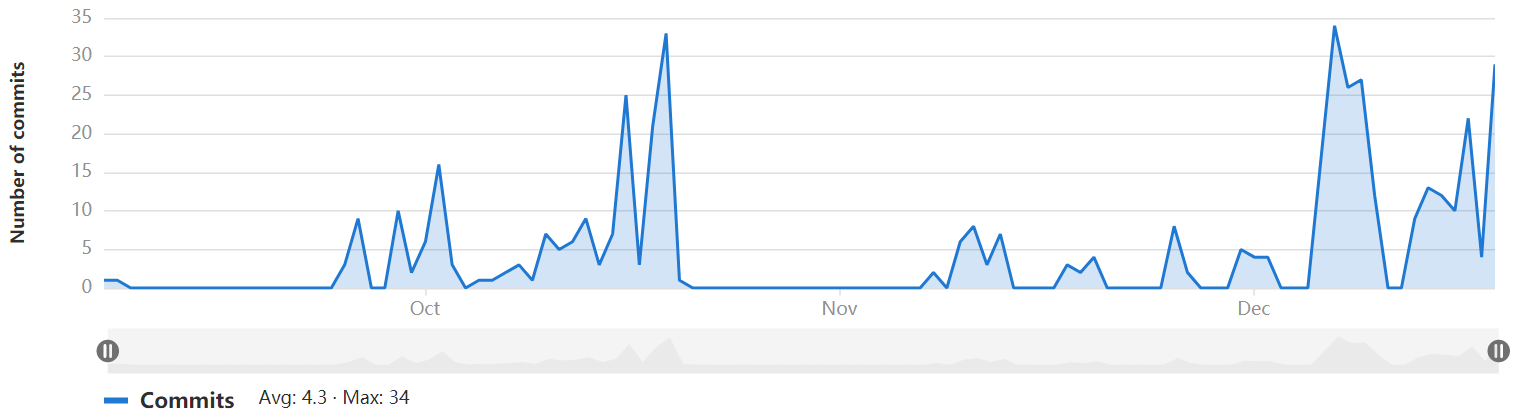
\includegraphics[width=15cm]{slike/dijagrampregledapromjena.PNG}
			\end{center}
			\caption{Dijagram pregleda promjena na grani Master}
			\label{fig:master}
		\end{figure}
		
		\begin{figure}[H]
			\begin{center}
				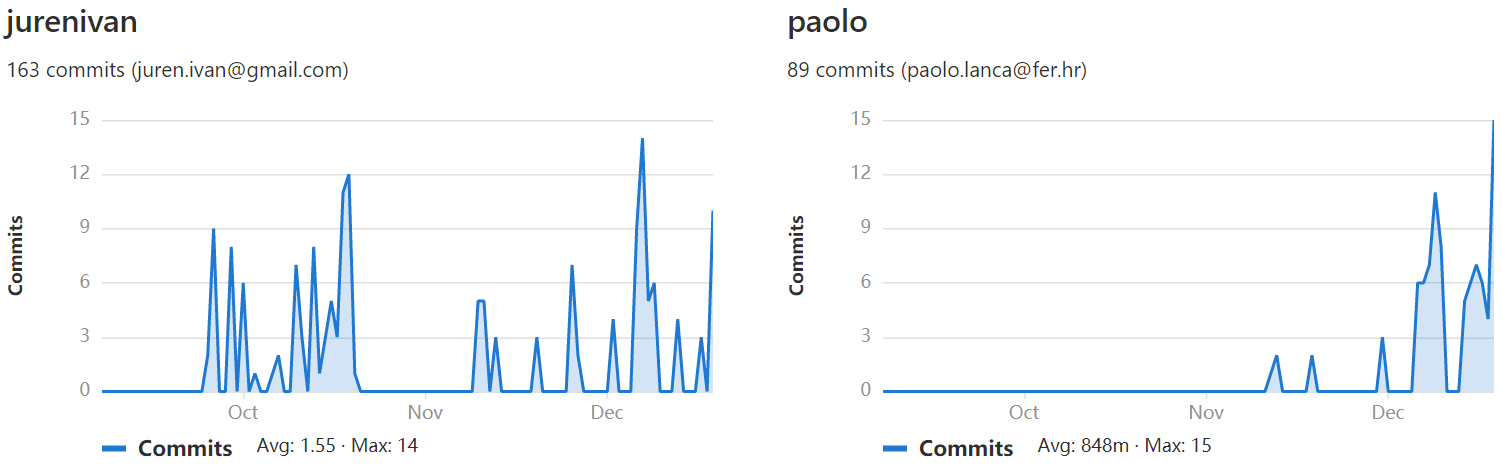
\includegraphics[width=15cm]{slike/dijagrampregledapromjena1.PNG}
				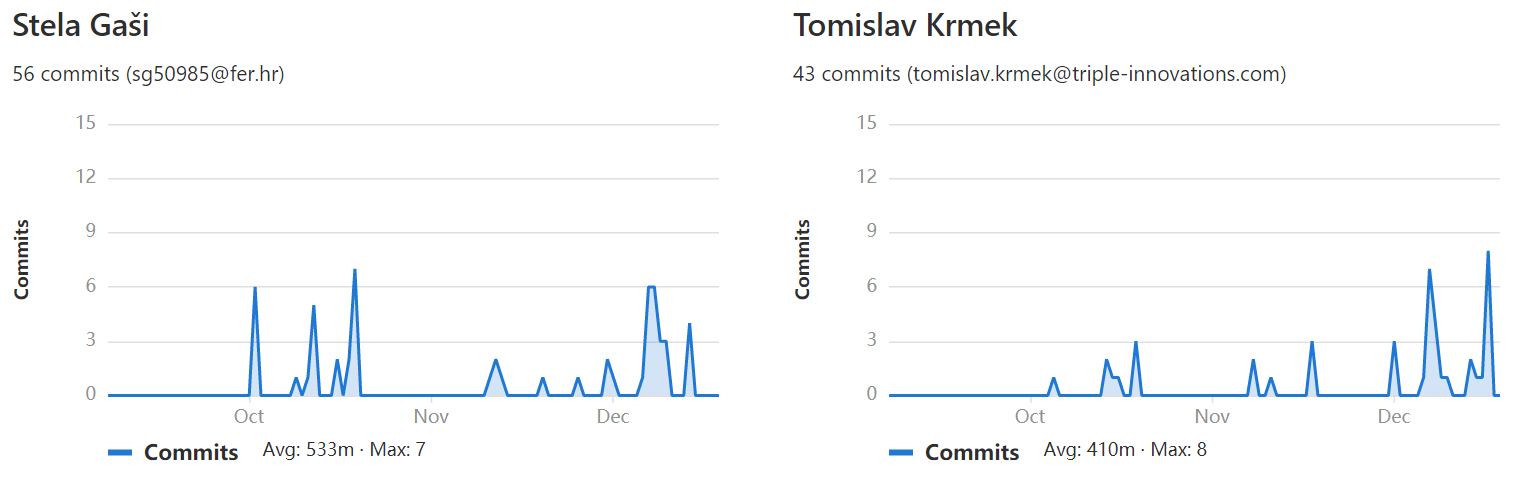
\includegraphics[width=15cm]{slike/dijagrampregledapromjena2.PNG}
				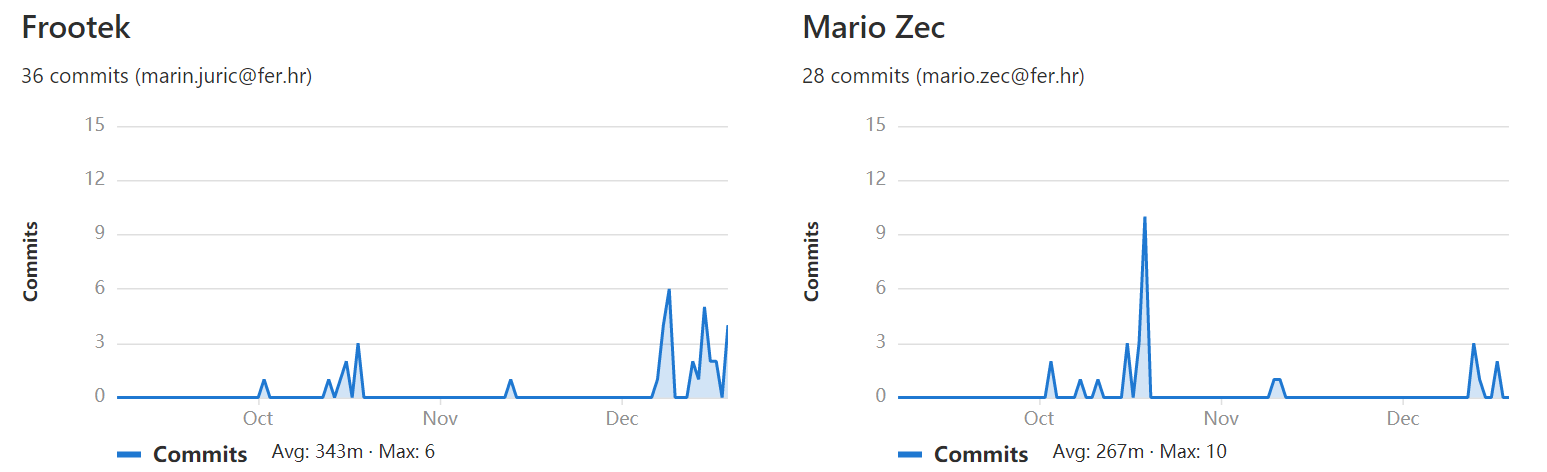
\includegraphics[width=15cm]{slike/dijagrampregledapromjena3.PNG}
				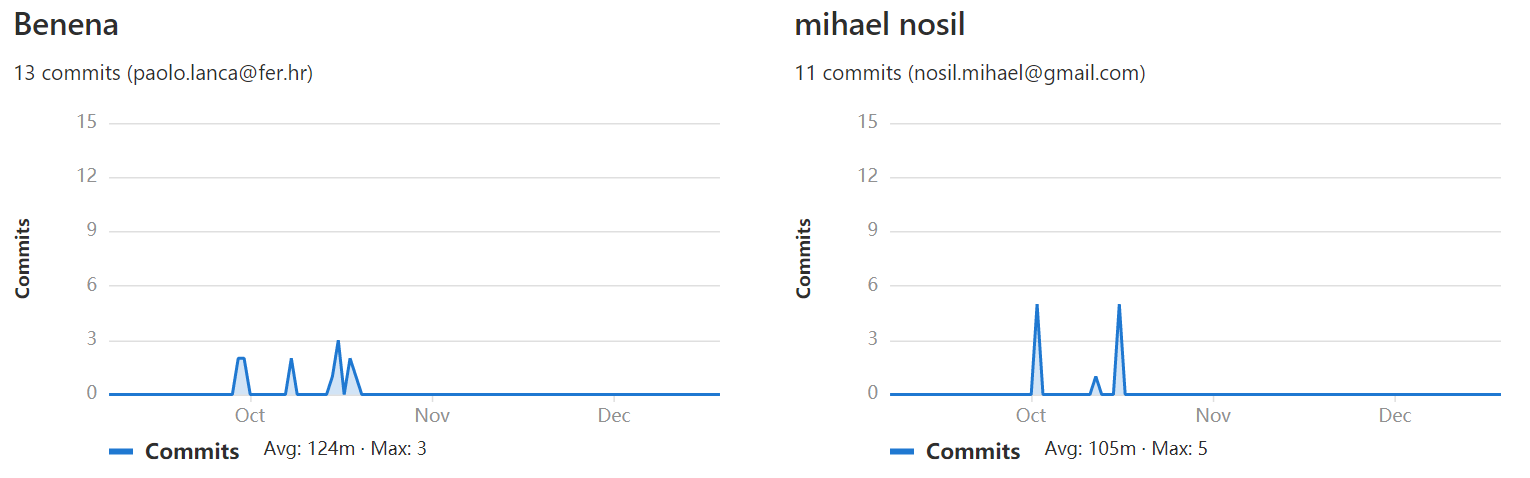
\includegraphics[width=15cm]{slike/dijagrampregledapromjena4.PNG}
				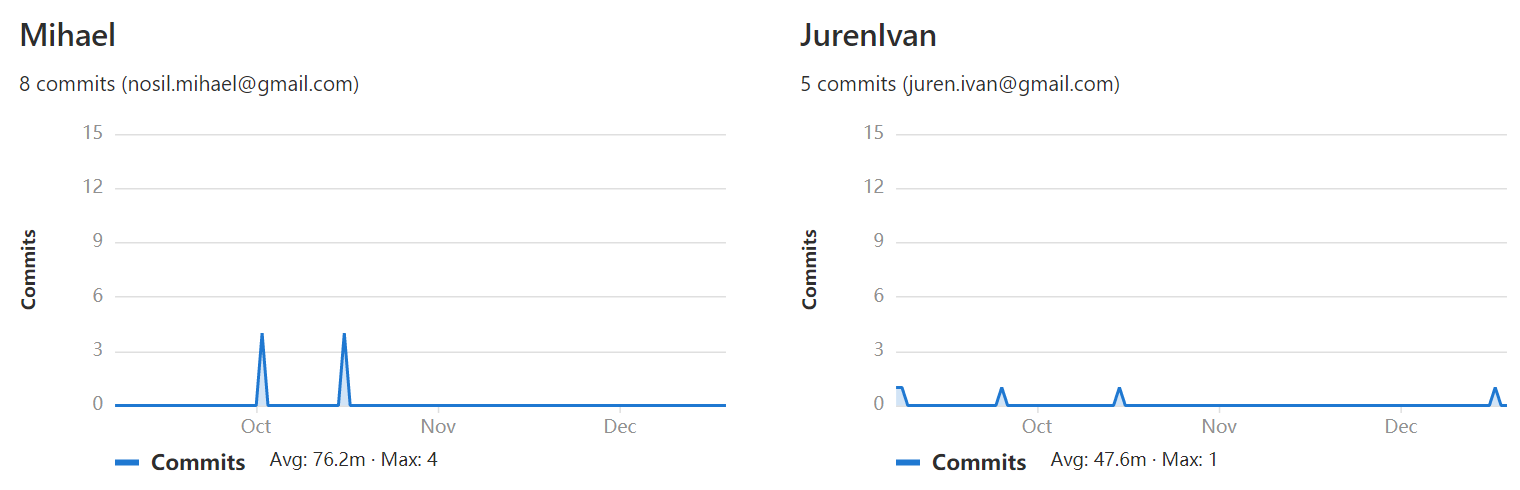
\includegraphics[width=15cm]{slike/dijagrampregledapromjena5.PNG}
			\end{center}
			\label{fig:dijapre}
		\end{figure}



>>>>>>> 0b35394bb8895deb759dc579f2583fe27a8564e1
\end{document}